\newpage
\section{GIẢI TAM GIÁC VÀ ỨNG DỤNG THỰC TẾ}
\subsection{LÝ THUYẾT CẦN NHỚ}
    \subsubsection{Định lí côsin}
\begin{dl}
	Trong tam giác $ABC$, ta kí hiệu $A$, $B$, $C$ là các góc của tam giác tại đỉnh tương ứng; $a$, $b$, $c$ tương ứng là độ dài của các cạnh đối diện với đỉnh $A$, $B$, $C$. Khi đó
	\begin{multicols}{3}
		\begin{itemize}
			\item $a^2=b^2+c^2-2bc\cos A$,
			\item $b^2=c^2+a^2-2ca\cos B$,
			\item $c^2=a^2+b^2-2ab\cos C$.
		\end{itemize}
	\end{multicols}
\end{dl}
\begin{note}
	Từ Định lí côsin, ta tính được $\cos A$, $\cos B$, $\cos C$ theo độ dài các cạnh $a$, $b$, $c$ của tam giác $ABC$, cụ thể:
	\begin{multicols}{3}
		\begin{itemize}
			\item $\cos A=\dfrac{b^2+c^2-a^2}{2bc}$.
			\item $\cos B=\dfrac{a^2+c^2-b^2}{2ac}$.
			\item $\cos C=\dfrac{a^2+b^2-c^2}{2ab}$.
		\end{itemize}
	\end{multicols}
	
\end{note}

\begin{dn}
\textbf{Giải tam giác} là quá trình xác định đầy đủ các cạnh và góc của một tam giác, dựa vào một số thông tin ban đầu đã biết (các cạnh và/hoặc các góc). Nói cách khác, nếu bạn biết một số yếu tố của tam giác (cạnh, góc) thì bạn có thể dùng các định lý hình học để tìm ra các yếu tố còn lại.\\
Các công cụ để giải tam giác: Định lý về tổng ba góc trong một tam giác, định lý sin, định lý côsin.
\end{dn}	
	
\subsubsection{Định lí sin}
\begin{dl}
	Trong tam giác $ABC$, ta kí hiệu $A$, $B$, $C$ là các góc của tam giác tại đỉnh tương ứng; $a$, $b$, $c$ tương ứng là độ dài của các cạnh đối diện với đỉnh $A$, $B$, $C$. $R$ là bán kính đường tròn ngoại tiếp tam giác $ABC$. Khi đó
	$$\dfrac{a}{\sin A}=\dfrac{b}{\sin B}=\dfrac{c}{\sin C}=2R.$$
\end{dl}
\subsubsection{Công thức tính diện tích tam giác}

	Trong tam giác $ABC$, ta kí hiệu $A$, $B$, $C$ là các góc của tam giác tại đỉnh tương ứng; $a$, $b$, $c$ tương ứng là độ dài của các cạnh đối diện với đỉnh $A$, $B$, $C$; $p$ là nửa chu vi; $S$ là diện tích; $R$, $r$ tương ứng là bán kính đường tròn ngoại tiếp, nội tiếp tam giác $ABC$. Khi đó
	\begin{multicols}{2}
		\begin{itemize}
			\item $S=pr=\dfrac{(a+b+c)r}{2}$;   
			\item $S=\dfrac{1}{2}bc\sin A=\dfrac{1}{2}ca\sin B=\dfrac{1}{2}ab\sin C$;
			\item $S=\dfrac{abc}{4R}$;
			\item $S=\sqrt{p(p-a)(p-b)(p-c)}$;
			\item $S=\dfrac{1}{2}ah_a=\dfrac{1}{2}bh_b=\dfrac{1}{2}ch_c.$
		\end{itemize}
	\end{multicols}

\subsection{PHÂN LOẠI VÀ PHƯƠNG PHÁP GIẢI TOÁN}
\begin{dang}{Giải tam giác và ứng dụng thực tế}
	Việc tính độ dài các cạnh và số đo các góc của một tam giác khi biết một số yếu tố của tam giác đó được gọi là giải tam giác.  \\
	Áp dụng các định lí côsin, sin và sử dụng máy tính cầm tay, ta có thể tính (gần đúng) các cạnh và các góc của một tam giác trong các trường hợp sau
	\begin{itemize}
		\item Biết hai cạnh và góc xen giữa;
		\item Biết ba cạnh;
		\item Biết một cạnh và hai góc;
		\item Hai cạnh và 1 góc bất kỳ.
	\end{itemize}
\end{dang}
\setcounter{subsubsection}{0}
\setcounter{ex}{0}
\setcounter{bt}{0}
\setcounter{vd}{0}
\begin{vd}%[0H4N3-1]%[Dự án đề cương 3 khối NH24-25 - Đợt 2 - Vũ Ngọc Hào]
	Cho tam giác $ABC$ có $\widehat{B}=60^\circ$, $\widehat{C}=45^\circ$, $AC=10$. Tính $a$, $R$, $S$, $r$ (kết quả làm tròn đến hàng phần mười).
	\loigiai{
		Ta có $\widehat{A}=180^\circ-\widehat{B}-\widehat{C}=75^\circ$.\\
		Áp dụng định lý sin $\dfrac{BC}{\sin A}=\dfrac{AC}{\sin B}$. Suy ra $BC=\dfrac{AC\cdot \sin A}{\sin B}=\dfrac{10\cdot \sin 75^\circ}{\sin 60^\circ}=\dfrac{5\sqrt{6}+15\sqrt{2}}{3}\approx 11{,}2 $.\\
		Ta có $\dfrac{AC}{\sin B}=2R$. Suy ra $R=\dfrac{AC}{2\sin B}=\dfrac{10\sqrt{3}}{3}\approx 5{,}8$.    \\
		Diện tích tam giác $ABC$ là $S=\dfrac{1}{2}BC\cdot AC\cdot \sin C=\dfrac{1}{2}\cdot \left(\dfrac{5\sqrt{6}+15\sqrt{2}}{3}\right)\cdot 10\cdot \sin 45^\circ=\dfrac{75+25\sqrt{3}}{3}\approx 39{,}4$.\\
		Ta có $\dfrac{AB}{\sin C}=\dfrac{AC}{\sin B}$. Suy ra $AB=\dfrac{AC\cdot \sin C}{\sin B}=\dfrac{10\sqrt{6}}{3}\approx 8{2}2$.\\
		Tam giác $ABC$ có nửa chu vi là $p=\dfrac{AB+BC+AC}{2}\approx 14{,}7$.\\
		Mà $S=pr$. Suy ra $r=\dfrac{S}{p}\approx 2{,}7$.
	}
\end{vd}
\begin{vd}%[0H4H3-1]%[Dự án đề cương 3 khối NH24-25 - Đợt 2 - Vũ Ngọc Hào]
	Cho tam giác $ABC$ có $AB=9$, $BC=12$, $AC=16$.  Tính các góc $A$, $B$, $C$  của tam giác đó và diện  tích tam giác $ABC$ (làm tròn kết quả đến hàng phần trăm).
	\loigiai{
		Áp dụng định lí côsin trong $\triangle ABC$ ta có
		\begin{eqnarray*}
			& &BC^2=AB^2+AC^2-2AB \cdot AC \cos A \\
			& \Leftrightarrow & \cos A=\dfrac{AB^2+AC^2- BC^2}{2AB \cdot AC}\\
			& \Leftrightarrow & \cos A=\dfrac{9^2+16^2-12^2}{2 \cdot 9 \cdot 16}= \dfrac{193}{288}\\
			&\Rightarrow& \widehat{A} \approx 47{,}92^\circ.
		\end{eqnarray*}
		Tương tự
		\[ \cos B=\dfrac{9^2+12^2-16^2}{2 \cdot 9 \cdot 12}=- \dfrac{31}{216}  \Rightarrow \widehat{B}  \approx 98{,}25^\circ.\]
		Khi đó $\widehat{C}= 180^\circ-\widehat{A} -\widehat{B}=180^\circ-47{,}92^\circ- 98{,}25^\circ=33{,}83^\circ$. \\
		Ta có $p=\dfrac{AB+AC+BC}{2}=\dfrac{9+12+16}{2}=\dfrac{37}{2}$.\\
		Khi đó diện tích tam giác $ABC$ là
		$$S_{\triangle ABC}=\sqrt{p(p-AB)(p-AC)(p-BC)}=\sqrt{\dfrac{37}{2}\left(\dfrac{37}{2}-9\right)\left(\dfrac{37}{2}-12\right)\left(\dfrac{37}{2}-16\right)}\approx 53{,}44 \mathrm{~(\text{đvdt})}.$$
	}
\end{vd}
\begin{vd}%[0H4V3-1]%[Dự án đề cương 3 khối NH24-25 - Đợt 2 - Vũ Ngọc Hào]
	\immini{
		Cho tam giác $ABC$ có $AB=12$, $AC=9$, $\widehat{A}=60^{\circ}$. $M$ là điểm thuộc cạnh $AB$  sao cho $AM=2BM$. Tính cạnh $CM$ và  góc $\widehat{BCM}$ (làm tròn kết quả đến hàng phần mười).
	}
	{
		\begin{tikzpicture}[scale=1, font=\footnotesize, line join=round, line cap=round,>=stealth]
			\path
			(0,0) coordinate (A)
			(4,0) coordinate (B)
			;
			\coordinate (M) at ($(A)!{2/3}!(B)$) ;
			\coordinate (C) at ($(A)+(60:3)$) ;
			\draw (A)--(B)--(C)--(A) (C)--(M)
			pic["$60^{\circ}$", draw=black, angle eccentricity=1.5, angle radius=0.7cm]{angle=B--A--C};
			\foreach \x/\g in {A/-120,B/-60,C/90,M/-90}
			\fill[black] (\x) circle (1pt)+(\g:3mm) node {$\x$};
		\end{tikzpicture}
	}
	\loigiai{
		Ta có $AM=2BM \Rightarrow BM=\dfrac{1}{3}AB=4$ và $AM=\dfrac{2}{3}AB=8$. \\
		Áp dụng định lí côsin trong $\triangle ABC$ ta có
		\begin{align*}
			&CM^2=AM^2+AC^2-2AM \cdot AC \cos A=8^2+9^2-2 \cdot 8 \cdot 9 \cos 60^\circ=73 \Rightarrow CM=\sqrt{73} \approx 8{,}5; \\
			&BC^2=AB^2+AC^2-2AB \cdot AC \cos A=12^2+9^2-2 \cdot 12 \cdot 9 \cos 60^\circ=117\Rightarrow BC=\sqrt{117}.
		\end{align*}
		Áp dụng định lí côsin ta có
		\begin{eqnarray*}
			&&BM^2=CM^2+CB^2-2CM \cdot CB \cos \widehat{BCM}  \\
			&\Leftrightarrow & \cos \widehat{BCM}=\dfrac{CM^2+CB^2- BM^2}{2CM \cdot CB}  \\
			&\Leftrightarrow & \cos \widehat{BCM}=\dfrac{73+117-16}{2 \cdot \sqrt{73} \cdot \sqrt{117}}= \dfrac{29}{\sqrt{949}}\\
			&\Rightarrow& \widehat{BCM} \approx 19{,}7^\circ.
		\end{eqnarray*}
	}
\end{vd}
\begin{dang}{Ứng dụng thực tế}
Áp dụng định lý sin, định lý cosin, công thức tính diện tích và các yếu tố hình học khác để giải các bài toán ứng dụng thực tế.
\end{dang}
\setcounter{subsubsection}{0}
\setcounter{ex}{0}
\setcounter{bt}{0}
\setcounter{vd}{0}
\begin{vd}%[0H4H3-2]%[Dự án đề cương 3 khối NH24-25 - Đợt 2 - Vũ Ngọc Hào]
	\immini{
		Hai chiếc tàu thủy rời cảng ở cùng một thời điểm, theo hai hướng tạo với nhau góc $30^\circ$  (hình vẽ). Tàu T1 chạy  với vận tốc trung bình $30$ hải lý/giờ, tàu T2 chạy  với vận tốc trung bình $25$ hải lý/giờ. Hỏi sau $90$ phút, hai tàu cách nhau khoảng bao nhiêu hải lý (kết quả làm tròn đến hàng phần trăm)?
	}
	{
		\begin{tikzpicture}[scale=1, font=\footnotesize, line join=round, line cap=round,>=stealth]
			\path
			(0,0) coordinate (A)
			(4,0) coordinate (B)
			;
			\coordinate (C) at ($(A)+(30:3)$) ;
			\draw (A)--(B)--(C)--(A)
			pic["$30^{\circ}$", draw=black, angle eccentricity=1.5, angle radius=0.7cm]{angle=B--A--C};
			\draw ($(A)!0.5!(B)$) node[below]{$\mathrm{T1}$} ($(A)!0.5!(C)$) node[above]{$\mathrm{T2}$};
			\foreach \x/\g in {A/-120,B/-60,C/90}
			\fill[black] (\x) circle (1pt)+(\g:3mm) node {$\x$};
		\end{tikzpicture}
	}
	\loigiai{
		Giả sử hai tàu xuất phát từ điểm $A$. Sau 90 phút, tàu T1 đi được đến điểm $B$ và tàu T2 đi được đến điểm $C$.  \\
		Ta có
		$AB= 30 \cdot 1{,}5=45$; $AC= 25 \cdot 1{,}5=37{,}5$ và $\widehat{BAC}=30^{\circ}$.\\
		Áp đụng định lí côsin ta có
		\begin{eqnarray*}
			BC &=& \sqrt{AB^2+AC^2-2 \cdot AB \cdot AC \cdot \cos 30^{\circ}}\\
			&=& \sqrt{45^2+37{,}5^2-2 \cdot 45 \cdot 37{,}5\cdot \cos 30^{\circ}} \\
			& \approx&  22{,}55.
		\end{eqnarray*}
		Vậy hai tàu cách nhau khoảng $22{,}55$ hải lý.
	}
\end{vd}

\begin{vd}%[0H4N3-2]%[Dự án đề cương 3 khối NH24-25 - Đợt 2 - Vũ Ngọc Hào]
	\immini{
		Ở giữa một cái hồ có một cái đảo nhỏ. Để tính khoảng cách từ điểm $A$ trên đảo đến điểm $B$ trên bờ hồ, người ta chọn điểm $C$. Sau đó thực hiện đo các góc $B$, $C$ và khoảng cách $BC$. Biết $\widehat{B}=88^\circ$, $\widehat{C}=85^\circ$ và $BC=50$ m. Tính khoảng cách từ $A$ đến $B$ (kết quả làm tròn đến hàng phần mười).
	}
	{
		\begin{tikzpicture}[scale=1, font=\footnotesize, line join=round, line cap=round,>=stealth]
			\path
			(-0.3,0) coordinate (A)
			(-1,-2) coordinate (B)
			(1,-2) coordinate (C)
			;
			\draw[fill=cyan!30] (0.5,0) ellipse (2.5cm and 1.cm);
			\draw[fill=gray!30] (0,0) ellipse (0.5cm and 0.2cm);
			\draw (A)--(B)--(C)--(A) ;
			\draw pic["$85^{\circ}$", draw=black, angle eccentricity=1.6, angle radius=0.4cm]{angle=A--C--B} ;
			\draw pic["$88^{\circ}$", draw=black, double, angle eccentricity=1.9, angle radius=0.3cm]{angle=C--B--A};
			\foreach \x/\g in {A/120,B/-120,C/-60}
			\fill[black] (\x) circle (1pt)+(\g:3mm) node {$\x$};
		\end{tikzpicture}
	}
	\loigiai{
		Ta có $\widehat{A}=180^\circ-\widehat{B}-\widehat{C}=180-88^\circ-85^\circ=7^\circ$. \\
		Áp dụng định lí sin trong $\triangle ABC$ ta có
		\begin{align*}
			\dfrac{AB}{\sin C}=\dfrac{BC}{\sin A} \Rightarrow AB=\dfrac{BC\sin C}{\sin A}=\dfrac{50 \sin 85^{\circ}}{\sin 7^\circ}  \approx 408{,}7.
		\end{align*}
		Vậy $AB= 408{,}7$ m.
	}
\end{vd}

\begin{vd}%[0H4H3-2]%[Dự án đề cương 3 khối NH24-25 - Đợt 2 - Vũ Ngọc Hào]
	\immini{
		Từ một vị trí quan sát $A$, một người nhìn đỉnh $B$ và chân $C$ của nhà cao tầng với các góc tương ứng là $43^{\circ}$ và $16^{\circ}$ so với phương nằm ngang. Biết chiều cao của tòa nhà là $18$ m, tính khoảng cách từ $A$ đến $C$ (kết quả làm tròn kết quả đến hàng phần mười).
	}
	{
		\begin{tikzpicture}[scale=0.8,>=stealth, font=\footnotesize, line join=round, line cap=round]
			\path
			(0,0) coordinate (A)
			(4,3) coordinate (B)
			(4,-1) coordinate (C)
			(4,0) coordinate (H)
			;
			\draw[pattern=bricks,pattern color=brown] (B)--(6,3)--(6,-1)--(4,-1)--(B);
			\foreach \i in {2,3,4,5}
			\draw[fill=white] ({4+1/3},{-1+(2/3)*(\i-1)})--({4+1/3},{-1+(2/3)*(\i-1)+0.5})--({4+2/3},{-1+(2/3)*(\i-1)+0.5})--({4+2/3},{-1+(2/3)*(\i-1)})--cycle
			({5+1/3},{-1+(2/3)*(\i-1)})--({5+1/3},{-1+(2/3)*(\i-1)+0.5})--({5+2/3},{-1+(2/3)*(\i-1)+0.5})--({5+2/3},{-1+(2/3)*(\i-1)})--cycle;
			\draw[dashed](A)--(B)  (A)--(C) (A)--(H);
			\draw pic["$43^{\circ}$", draw=black, angle eccentricity=1.4, angle radius=0.9cm]{angle=H--A--B};
			\draw pic["$16^{\circ}$", draw=black,double, angle eccentricity=1.5, angle radius=1.2cm]{angle=C--A--H};
			\foreach \x/\g in {A/180,B/90,C/140,H/145}
			\fill[black] (\x) circle (1pt)+(\g:3mm) node {$\x$};
			\clip (-0.5,{-1-0.25}) rectangle (6.6,-1) ;
			\draw[fill=gray!30] (-0.5,-1)--(6.6,-1)--(6.6,{-1-0.25})--(-0.5,{-1-0.25})--cycle;
			\foreach \i in {1,2,...,35}
			\draw ({-0.5+0.2*(\i)},-1)--($({-0.5+0.2*(\i)},-1)+(-120:0.3)$) ;
		\end{tikzpicture}
	}
	\loigiai{
	Trong $\triangle ABH$, ta có $AH=BH\cdot \cot \widehat{BAH}=CH\cdot  \cot \widehat{CAH}$. \\
		Suy ra
		\begin{eqnarray*}
			&&(BC-CH)\cdot  \cot \widehat{BAH}=CH \cot \widehat{CAH}\\
			&\Leftrightarrow & CH=\dfrac{BC \cdot \cot \widehat{BAH}}{\cot \widehat{CAH} +\cot \widehat{BAH} } \\
			&\Leftrightarrow & CH= \dfrac{18 \cdot \cot 43^\circ}{ \cot 16^\circ+\cot 43^\circ}.
		\end{eqnarray*}
		Khoảng cách từ $A$ đến $C$ là
		\[ AC=\dfrac{CH}{\sin 16^\circ}=\dfrac{18\cdot \cot 43^\circ}{ (\cot 16^\circ+ \cot 43^\circ)\sin 16^\circ} \approx 15{,}4\mathrm{~m}.\]
	}
\end{vd}
\begin{vd}%[0H4H3-2]%[Dự án đề cương 3 khối NH24-25 - Đợt 2 - Vũ Ngọc Hào]
	\immini{
		Để đo bán kính của một chiếc đĩa cổ chỉ còn lại một phần, các nhà khảo cổ lấy $3$ điểm trên chiếc đĩa (hình vẽ). Biết $AB=6{,}1$ cm, $BC=12$ cm, $AC=16{,}8$ cm, tính bán kính của chiếc đĩa (làm tròn kết quả đến hàng phần mười).
	}
	{
		\begin{tikzpicture}[scale=1, font=\footnotesize, line join=round, line cap=round,>=stealth]
			\coordinate (O) at (0,0);
			\coordinate (A) at ($(O)+(131.4:3)$) ;
			\coordinate (B) at ($(O)+(101.6:3)$) ;
			\coordinate (C) at ($(O)+(41.7:3)$) ;
			\coordinate (D) at ($(O)+(140:3)$) ;
			\coordinate (E) at ($(O)+(90:1)$) ;
			\coordinate (F) at ($(O)+(18:3)$) ;
			\draw
			(D)
			.. controls ++(-10:0.5) and ++(180:0.5) .. (E)
			.. controls ++(180:-0.5) and ++(160: 0.5) .. (F)
			;
			\draw (A)--(B)--(C)--(A)  ;
			\draw  (F) arc (18:140:3);
			\foreach \x/\g in {A/140,B/90,C/60}
			\fill[black] (\x) circle (1.1pt)+(\g:3mm) node {$\x$};
		\end{tikzpicture}
	}
	\loigiai{
		Áp dụng định lí côsin ta có
		\begin{align*}
			&BC^2=AB^2+AC^2-2AB \cdot AC \cos A  \\
			\Leftrightarrow~ & \cos A=\dfrac{AB^2+AC^2- BC^2}{2AB \cdot AC}  \\
			\Leftrightarrow~ & \cos A=\dfrac{6{,}1^2+16{,}8^2-12^2}{2 \cdot 6{,}1 \cdot 16{,}8}= 0{,}85602\\
			\Rightarrow~& \widehat{A} \approx 32^\circ.
		\end{align*}
		Áp dụng định lí sin suy ra bán kính của chiếc đĩa là
		\[
		R=\dfrac{BC}{2\sin A}=\dfrac{12}{2\sin 32^\circ} \approx 11{,}3 \mathrm{~(cm)}.
		\]
	}
\end{vd}
\subsection{Bài tập rèn luyện}
\ind{PHẦN I.} \inden{Câu trắc nghiệm nhiều phương án lựa chọn. Mỗi câu hỏi học sinh chỉ chọn một phương án.}\\
\setcounter{ex}{0}
\Opensolutionfile{ans}[ans/0H4-Bai3-TN]%--Đặt tên 2D1-Bai1-Dang1-TN
\begin{ex}[Trích đề thi GHKI trường THPT Tân Bình-TPHCM-NH24-25]%[0H4N2-1]%[Dự án đề cương 3 khối NH24-25 - Đợt 2 - Vũ Ngọc Hào]
	Cho tam giác $ABC$ có $BC=a$, $AC=b$, $AB=c$. Mệnh đề nào sau đây đúng?
	\choice
	{$\cos A=\dfrac{b^2+c^2+a^2}{bc}$}
	{\True $\cos A=\dfrac{b^2+c^2-a^2}{2bc}$}
	{$\cos A=\dfrac{b^2+c^2+a^2}{2bc}$}
	{$\cos A=\dfrac{b^2+c^2-a^2}{bc}$}
	\loigiai{ 
		Công thức đúng của $\cos A$ trong tam giác là $\cos A=\dfrac{b^2+c^2-a^2}{2bc}$.
	}
\end{ex}


\begin{ex}[Trích đề thi GHKI trường THPT Tân Bình-TPHCM-NH24-25]%[0H4N2-1]%[Dự án đề cương 3 khối NH24-25 - Đợt 2 - Vũ Ngọc Hào]
	Tam giác $A B C$ có $a=8$, $c=3$, $\widehat{B}=60^{\circ}$. Độ dài cạnh $b$ bằng bao nhiêu?
	\choice 
	{\True $7$}
	{$\sqrt{61}$}
	{$\sqrt{97}$}
	{$49$}
	\loigiai{
		Áp dụng định lí côsin trong tam giác $ABC$ ta được
		$$b^2=a^2+c^2-2ac\cos \widehat{B}=8^2+  3^2-2\cdot8\cdot3\cdot\cos 60^{\circ}=49 \Rightarrow b=7.$$
	}
\end{ex}
\begin{ex}[Trích đề thi GHKI trường THPT Nguyễn Bỉnh Khiêm Cầu Giấy- Tp Hà Nội-NH24-25]%[0H4H2-1]%[Dự án đề cương 3 khối NH24-25 - Đợt 2 - Vũ Ngọc Hào]
	Tam giác $ABC$ có $\widehat{B}=30^{\circ}$, $\widehat{C}=45^{\circ}$ và $AB=5$. Tính độ dài cạnh $AC$.
	\choice
	{$AC=\dfrac{5\sqrt{6}}{2}$}
	{$AC=\dfrac{5\sqrt{3}}{2}$}
	{\True $AC=\dfrac{5\sqrt{2}}{2}$}
	{$AC=5\sqrt{2}$}
	\loigiai{
		\immini
		{
			Theo định lý Sin, ta có $\dfrac{AC}{\sin B}=\dfrac{AB}{\sin C}$ \\
			$\Rightarrow AC=\dfrac{AB\sin B}{\sin C}=\dfrac{5\sin 30^{\circ}}{\sin 45^{\circ}}=\dfrac{5\sqrt{2}}{2}$.
		}
		{
			\begin{tikzpicture}[line cap=round,line join=round,scale=1,font=\footnotesize]
				\path 
				(-3,0) coordinate (B)
				(2,0) coordinate (C)
				($(B)!.7!30:(C)$) coordinate (M)
				($(C)!.6!-45:(B)$) coordinate (N)
				coordinate (A) at (intersection of B--M and C--N)
				;
				\draw (A)--node[midway,above]{$5$}(B)--(C)--cycle;
				\foreach \i/\g in {A/90,B/180/,C/0} \fill (\i) circle (1pt) node[shift=(\g:0.3)]{$\i$};
				\pic[draw,angle radius=5mm]{angle=C--B--A };
				\pic[draw,angle radius=5mm]{angle=A--C--B };
				\pic[draw,angle radius=6mm]{angle=A--C--B };
				\path (B)node[shift={(12:9mm)}]{$30^\circ$}
				(C)node[shift={(160:9mm)}]{$45^\circ$}
				;
			\end{tikzpicture}
		}
	}
\end{ex}

\begin{ex}[Trích đề thi GHKII trường THPT Nguyễn Bỉnh Khiêm Cầu Giấy- Tp Hà Nội-NH24-25]%[0H4H3-1]%[Dự án đề cương 3 khối NH24-25 - Đợt 2 - Vũ Ngọc Hào]
	Cho tam giác $ABC$ có $a=4$, $c=5$, $\widehat{B}=150^{\circ}$. Diện tích của tam giác $ABC$ bằng
	\choice
	{\True $5$}
	{$10\sqrt{3}$}
	{$5\sqrt{3}$}
	{$10$}
	\loigiai{
		\immini
		{
			Ta có $S_{ABC}=\dfrac{1}{2}ac\sin B=\dfrac{1}{2}\cdot 4 \cdot 5 \cdot \sin 150^{\circ}=5$.
		}
		{
			\begin{tikzpicture}[line cap=round,line join=round,scale=1,font=\footnotesize]
				\path 
				(-3,0) coordinate (A)
				(2,0) coordinate (C)
				($(A)!.7!30:(C)$) coordinate (M)
				($(C)!.6!-45:(A)$) coordinate (N)
				coordinate (B) at (intersection of A--M and C--N)
				;
				\draw (A)--node[midway,above]{$5$}(B)--node[midway,above]{$4$}(C)--cycle;
				\foreach \i/\g in {A/180,B/90/,C/0} \fill (\i) circle (1pt) node[shift=(\g:0.3)]{$\i$};
				\pic[draw,angle radius=4mm]{angle=A--B--C };
				\path (B)node[shift={(-90:7mm)}]{$150^\circ$};
			\end{tikzpicture}
		}
	}
\end{ex}

\begin{ex}%[0H4N3-1]%[Dự án đề cương 3 khối NH24-25 - Đợt 2 - Vũ Ngọc Hào]
	Cho $\triangle ABC$ có $AB=6$ cm, $BC=7$ cm, $CA=8$ cm. Giá trị của $\cos B$ là
	\choice
	{$\dfrac{1}{2}$}
	{\True $\dfrac{1}{4}$}
	{$\dfrac{17}{32}$}
	{$\dfrac{11}{16}$}
	\loigiai{
	Ta có $\cos B=\dfrac{AB^2+BC^2-AC^2}{2\cdot AB\cdot BC}=\dfrac{6^2+7^2-8^2}{2\cdot 6\cdot 7}=\dfrac{1}{4}$.
	}
\end{ex}

\begin{ex}%[0H4N3-1]%[Dự án đề cương 3 khối NH24-25 - Đợt 2 - Vũ Ngọc Hào]
	Cho tam giác $ABC$ có góc $\widehat{B}=60^{\circ}, \widehat{C}=45^{\circ}$, $AB=9$. Độ dài cạnh $AC$ là
	\choice
	{$\dfrac{6\sqrt{6}}{2}$}
	{$3\sqrt{6}$}
	{\True $\dfrac{9\sqrt{6}}{2}$}
	{$\dfrac{4\sqrt{6}}{3}$}
	\loigiai{
		Áp dụng định lí sin ta có
		\[ \dfrac{AC}{\sin B}=\dfrac{AB}{\sin C} \Rightarrow AC=\dfrac{AB\cdot\sin B}{\sin C}=\dfrac{9\cdot \sin 60^\circ}{\sin 45^\circ}=\dfrac{9\sqrt{6}}{2}.\]
	}
\end{ex}
\begin{ex}[Trích đề thi GHKII trường THPT Nguyễn Bỉnh Khiêm Cầu Giấy- Tp Hà Nội-NH24-25]%[0H4N2-1]%[Dự án đề cương 3 khối NH24-25 - Đợt 2 - Vũ Ngọc Hào]
	Nếu tam giác $MNP$ có $MP=5$, $PN=8$, $\widehat{MPN}=120^\circ$ thì độ dài cạnh $MN$ bằng bao nhiêu (kết quả làm tròn đến hàng phần mười) ?
	\choice
	{\True $MN \approx 11{,}4$}
	{$MN \approx 12{,}0$}
	{$MN \approx 12{,}4$}
	{$MN \approx 7{,}0$}
	\loigiai{
		Áp dụng định lí cos cho $\triangle MNP$ ta có
		$$MN^2=PM^2+PN^2-2 \cdot PM \cdot PN \cdot \cos \widehat{MPN} \Rightarrow MN \approx 11{,}4.$$
	}
\end{ex}
\begin{ex}[Trích đề thi GHKII trường THPT Nguyễn Du Tp HCM-NH24-25]%[0H4N2-1]%[Dự án đề cương 3 khối NH24-25 - Đợt 2 - Vũ Ngọc Hào]
	Cho tam giác $ABC$ có cạnh $BC=5$, góc $\widehat{BAC}=60^{\circ}$ và $\widehat{ACB}=45^{\circ}$. Tính độ dài cạnh $AB$.
	\choice
	{$\dfrac{5 \sqrt{2}}{3}$}
	{$\dfrac{5 \sqrt{3}}{3}$}
	{\True $\dfrac{5 \sqrt{6}}{3}$}
	{$\dfrac{ \sqrt{6}}{3}$} 
	\loigiai{
	Áp dụng định lý sin trong tam giác $ABC$:
	\[\dfrac{AB}{\sin C}=\dfrac{BC}{\sin A}.\]
	Suy ra:
	\[AB=\dfrac{5 \sin 45^{\circ}}{\sin 60^{\circ}}=\dfrac{5\sqrt{6}}{3}.\]
	}
\end{ex}

\begin{ex}[Trích đề thi GHKII trường THPT Tây Thạnh-NH24-25]%[0H4N2-1]%[Dự án đề cương 3 khối NH24-25 - Đợt 2 - Vũ Ngọc Hào]
	Cho tam giác $ABC$ có $AB=6$, $AC=\sqrt{20}$, $B C=\sqrt{32}$. Tính góc $\widehat{B}$ của tam giác $AB C$.
	\choice
	{$\widehat{B}=90^{\circ}$}
	{$\widehat{B}=120^{\circ}$}
	{$\widehat{B}=60^{\circ}$}
	{\True $\widehat{B}=45^{\circ}$}
	\loigiai{
	Áp dụng định lí côsin cho tam giác $ABC$, ta có:\\
		$\cos B=\dfrac{AB^2+BC^2-AC^2}{2AB\cdot BC}=\dfrac{6^2+(\sqrt{32})^2-(\sqrt{20})^2}{2\cdot6\cdot\sqrt{32}}=\dfrac{\sqrt{2}}{2}$.\\
		Suy ra $\widehat{B}=45^\circ$.
	}
\end{ex}
\begin{ex}%[0H4H3-1]%[Dự án đề cương 3 khối NH24-25 - Đợt 2 - Vũ Ngọc Hào]
	\immini{
		Cho tam giác $ABC$ có các kích thước và góc như hình vẽ bên. Độ dài cạnh $AB$ bằng bao nhiêu?
		\choice
		{$20$ cm}
		{\True $21$ cm}
		{$25$ cm}
		{$35$ cm}
	}{
		\begin{tikzpicture}[scale=1,>=stealth, font=\footnotesize, line join=round, line cap=round]
			\coordinate (A) at (0,0);
			\coordinate (C) at (-2,0);
			\coordinate (B) at ($(C)+(41:3)$);
			\draw (A) -- (B) -- (C) -- cycle;
			\node[shift={(180:3mm)},rotate=41] at ($(B)!0.5!(C)$){$29$ cm};
			\node[shift={(-90:3mm)}] at ($(A)!0.5!(C)$){$13$ cm};
			\draw pic["$41^{\circ}$", draw=black, angle eccentricity=1.6, angle radius=0.6cm]{angle=A--C--B} ;
			\foreach \p/\g in {A/-90,B/45,C/-90}
			\fill (\p) circle (1.5pt) node[shift=(\g:3mm)] {$\p$};
		\end{tikzpicture}
	}
	\loigiai{
		Áp dụng định lý cô-sin trong tam giác $ABC$
		\allowdisplaybreaks
		\begin{eqnarray*}
			AB^2 &=& AC^2+BC^2-2 \cdot AC \cdot BC \cdot \cos 41^{\circ}\\
			&=& 13^2+29^2-2 \cdot 13 \cdot 29 \cdot \cos 41{\circ}\\
			&\approx& 440{,}95.
			\end{eqnarray*}
		Do đó $AB=\sqrt{440{,}95} \approx 21$ cm.
	}
\end{ex}
\begin{ex}[Trích đề thi GHKI trường THPT Tây Thạnh-NH24-25]%[0H4H3-1]%[Dự án đề cương 3 khối NH24-25 - Đợt 2 - Vũ Ngọc Hào]
	Một tam giác có ba cạnh là $52$, $56$, $60$. Bán kính đường tròn ngoại tiếp là
	\choice
	{$\dfrac{65}{8}$}
	{$40$ }
	{\True $32{,}5$}
	{$\dfrac{65}{4}$}
	\loigiai{
		Nửa chu vi của tam giác là $p=\dfrac{52+56+60}{2}=84$.\\
		Diện tích của tam giác là $S=\sqrt{84(84-52)(84-56)(84-60)}=1344$.\\
		Bán kính đường tròn ngoại tiếp của tam giác là $R=\dfrac{52\cdot56\cdot60}{4\cdot1344}=32{,}5$.
	}
\end{ex}
\begin{ex}%[0H4H3-1]%[Dự án đề cương 3 khối NH24-25 - Đợt 2 - Vũ Ngọc Hào]
	Cho tam giác $ABC$ có $AB=\sqrt{2}$, $\widehat{B}=60^{\circ}$, $\widehat{A}=75^{\circ}$. Độ dài cạnh $AC$ bằng
	\choice
	{\True $AC=\sqrt{3}$}
	{$AC=\dfrac{\sqrt{3}}{2}$}
	{$AC=3$}
	{$AC=\dfrac{\sqrt{3}}{3}$}
	\loigiai{
		\immini{
			Ta có: $\widehat{C}=180^{\circ}-\left(\widehat{B}+\widehat{A}\right)=180^{\circ}-\left(60^{\circ}+75^{\circ}\right)=45^{\circ}$.\\
			Theo định lý Sin ta có $\dfrac{AC}{\sin B}=\dfrac{AB}{\sin C}$.\\
			Suy ra $AC=\dfrac{AB\cdot\sin B}{\sin C}=\dfrac{\sqrt{2}\cdot\sin 60^{\circ}}{\sin 45^{\circ}}=\sqrt{3}.$}
		{\vspace{-0.5cm}
			\begin{tikzpicture}[scale=0.8,>=stealth, font=\footnotesize, line join=round, line cap=round]
				\path
				(0,0) coordinate (A) node [below]{$A$}
				(1,3) coordinate (B) node [above]{$B$}
				(3,0) coordinate (C) node [below]{$C$}
				;
				\draw (A)--(B)--(C)--cycle;
				\foreach \x in {A,B,C} \draw[fill=black] (\x) circle (1pt);
				\draw pic["$60^{\circ}$", draw=black, angle eccentricity=1.6, angle radius=0.4cm]{angle=A--B--C} ;
				\draw pic["$75^{\circ}$", draw=black, angle eccentricity=1.6, angle radius=0.4cm]{angle=C--A--B} ;
	\end{tikzpicture}}}
\end{ex}
\begin{ex}%[0H4H3-2]%[Dự án đề cương 3 khối NH24-25 - Đợt 2 - Vũ Ngọc Hào]
	Tam giác có độ dài ba cạnh là $3$, $8$, $9$. Góc lớn nhất của tam giác có số đo bằng bao nhiêu?
	\choice
	{$93{,}5^\circ$}
	{$88{,}6^\circ$}
	{\True $99{,}6^\circ$}
	{$101{,}3^\circ$}
	\loigiai{
		Góc lớn nhất $\alpha$ của tam giác là góc đối diện với cạnh lớn nhất của tam giác. \\
		Áp dụng định lí côsin ta có
		\[
		\cos \alpha=\dfrac{3^2+8^2-9^2}{2 \cdot 3 \cdot 8}=-\dfrac{1}{6} \Rightarrow \alpha \approx 99{,}6^\circ.
		\]
	}
\end{ex}
\begin{ex}%[0H4H3-1]%[Dự án đề cương 3 khối NH24-25 - Đợt 2 - Vũ Ngọc Hào]
	\immini
	{Trên sườn đồi có một cái cây thẳng đứng (tham khảo hình vẽ) đổ bóng dài $AB=39{,}5$ mét xuống đồi. Biết góc nghiêng của sườn đồi là $\alpha=26^{\circ}$ so với phương ngang và góc nâng của mặt trời là $\beta=50^{\circ}$.\\
	Chiều cao $BC$ của cây (làm tròn đến hàng đơn vị) là
	\choice
	{$21$ mét}
	{$27$ mét}
	{\True $25$ mét}
	{$23$ mét}
	}
	{
		\begin{tikzpicture}[line join=round, line cap=round,scale=1,transform shape]
			\clip (-1,-1) rectangle (6,6);
			\definecolor{cadmiumgreen}{rgb}{0.0, 0.42, 0.24}
			\path 
			(0,0) coordinate (A)	
			(4,2) coordinate (B)
			(4,0) coordinate (H)
			(4,4) coordinate (C)
			($(A)!1.3!(B)$) coordinate (D)
			($(A)!-0.3!(B)$) coordinate (E)
			($(A)!1.2!(C)$) coordinate (C1)
			($(A)!0.4!(B)$) coordinate (A1)
			($(A)!0.25!(B)$) coordinate (A2)
			;
			\draw [thick] (E)--(D);
			\draw [dashed] (A)--(H)--(C)--cycle (C)--(C1);
			\draw pic[draw=black, angle radius=.3cm]
			{right angle=A--H--B}; 
			\draw pic[draw,angle radius=0.8cm]{angle=H--A--B};
			\draw pic[draw,angle radius=1.3cm]{angle=H--A--C};
			\draw (A1) node[below] {$ \beta $};
			\draw (A2) node[below] {$ \alpha $};
			\foreach \x/\g in {A/-90, B/-45, C/90}
			\draw [fill=black] (\x) circle (.05)+(\g:.3) node {$\x$};
			
			%%%%%%%%%%%%%%%%%%%%%%%%%%%%%%%%%
			\tikzset{cay/.pic={%Cây
					\def\T{ 
						(-1.73,-2.85)
						..controls +(40:.03) and +(40:.01) ..  (-1.74,-2.7)
						..controls +(140:.04) and +(60:.02) ..  (-1.78,-2.6)
						..controls +(140:.04) and +(60:.02) ..  (-1.8,-2.55)
						..controls +(100:.03) and +(70:.02) ..  (-1.82,-2.5)
						..controls +(140:.04) and +(60:.02) ..  (-1.815,-2.4)
						..controls +(140:.04) and +(60:.02) ..  (-1.818,-2.3)
						..controls +(85:.03) and +(-30:.03) ..  (-1.8,-2.2)
						..controls +(80:.04) and +(50:.02) ..  (-1.78,-2)
						..controls +(60:.04) and +(120:.02) ..  (-1.76,-1.9)
						..controls +(80:.03) and +(-100:.02) ..  (-1.74,-1.8)
						..controls +(80:.01) and +(-100:.02) ..  (-1.72,-1.9)
						..controls +(60:.02) and +(-120:.02) ..  (-1.7,-2)
						..controls +(-80:.02) and +(110:.03) ..  (-1.66,-2.2)
						..controls +(-100:.02) and +(60:.03) ..  (-1.64,-2.3)
						..controls +(-30:.02) and +(70:.02) ..  (-1.6,-2.44)
						..controls +(-100:.02) and +(70:.02) ..  (-1.63,-2.52)
						..controls +(-60:.02) and +(70:.01) ..  (-1.66,-2.6)
						..controls +(60:.01) and +(70:.02) ..  (-1.7,-2.7)
						..controls +(-120:.02) and +(120:.03) ..  (-1.68,-2.85)
						;}
					\draw \T;
					\fill[cadmiumgreen!90!] \T;
			}}
			%%%%%%%%%%%%%%%%%%%%%%
			\tikzset{mat_troi/.pic={%Cây
					\def\T{
						(-3.5,4.5)--(-2,6)--(-.5,5) 
						(-1.5,4)--(-2,6)--(0,6.5) 
						(-4,6)--(-2,6)--(-1,7.7) (-2,6)--(-3,7.6);}
					\draw[orange,line width=1.5pt]\T;
					\draw[fill=orange] (-2,6) circle (25pt);
			}}
			\path 
			(9.2,7.18)pic[xscale=3,yscale=1.8]{cay}
			(5.6,2.5)pic[scale=.4]{mat_troi};
		\end{tikzpicture}
	}
	\loigiai{
		Theo hình vẽ ta thấy $\widehat{C A B}=\beta-\alpha=50^\circ-26^\circ=24^\circ, \widehat{A C B}=90^{\circ}-\beta=90^\circ-50^\circ=40^\circ$.\\
		Áp dụng định lý sin trong tam giác $ ABC $ ta có: $ \dfrac{BC}{\sin\widehat{CAB}}=\dfrac{AB}{\sin\widehat{ACB}} $.\\
		Suy ra $ BC= \dfrac{AB}{\sin\widehat{ACB}}\cdot \sin\widehat{CAB}=\dfrac{39{,5}}{\sin 40^\circ}\cdot \sin 24^\circ\approx 25 $ mét.
	}
\end{ex}
\begin{ex}[Trích đề thi GHKII trường THPT chuyên Lê Qúy Đôn Ninh Thuận-NH23-24]%[0H4H3-2]%[Dự án đề cương 3 khối NH24-25 - Đợt 2 - Vũ Ngọc Hào]
	\immini[thm]{Một trò chơi trên máy tính đang mô phỏng một vùng biển có hai hòn đảo nhỏ có toạ độ $B(50;30)$ và $C(32;-23)$. Một con tàu đang neo đậu tại điểm $A(-10;20)$. Số đo của góc  $\widehat{BAC}$ gần với số nào sau đây?
		\choice
		{$89^{\circ}3'$}
		{$45^{\circ}10'$}
		{$60^{\circ}7'$}
		{\True $55^{\circ}8'$}}{
		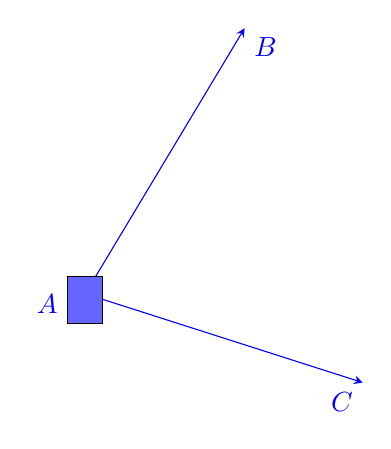
\begin{tikzpicture}[scale=1.5,>=stealth,line join=round,line cap=round]
			\draw[->, blue] (0,0)--(1.5,2.5) node[ below right,scale=1] {$B$};
			\draw[->, blue] (0,0.3)--(2.5,-0.5) node[ below left,scale=1] {$C$};
			\draw[ blue] (0,0) node[ above left,scale=1] {$A$};
			\fill[blue!60] (0,0) rectangle (0.3,0.4);
			\draw (0,0) rectangle (0.3,0.4);
	\end{tikzpicture}}
	\loigiai{
		Ta có $$AB=\sqrt{(50+10)^2+(30-20)^2}=10\sqrt{37};$$
		$$AC=\sqrt{(32+10)^2+(-23-20)^2}=\sqrt{3613};$$
		$$BC=\sqrt{(32-50)^2+(-23-30)^2}=\sqrt{3133}.$$
		Áp dụng định lí cô-sin trong tam giác $ABC$, ta có
		$$\cos\widehat{BAC}=\dfrac{AB^2+AC^2-BC^2}{2\cdot AB \cdot AC}=\dfrac{3700+3613-3133}{2\cdot 10\sqrt{37}\cdot \sqrt{3613}}\approx 0{,}57 $$ $$ \Rightarrow \widehat{BAC} \approx 55^{\circ}8'.$$
	}
\end{ex}
\begin{ex}%[0H4H3-2]%[Dự án đề cương 3 khối NH24-25 - Đợt 2 - Vũ Ngọc Hào]
	\immini{Tính khoảng cách giữa hai điểm ở hai đầu của một hồ nước. Biết từ một điểm cách hai đầu hồ lần lượt là $800$ m và $900$ m người quan sát nhìn hai điểm này dưới một góc $70^\circ$.
		\choice
		{$982$ m}
		{$879$ m}
		{\True $979$ m}
		{$882$ m}}{
		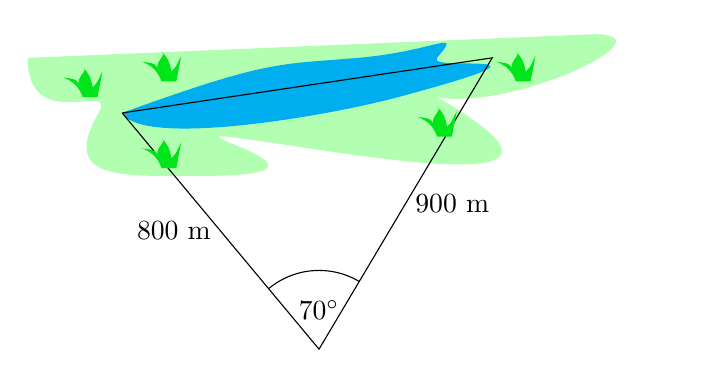
\begin{tikzpicture}
			\tikzset{co/.pic={
					\fill[green!80!teal,out=110,in=-20] (0,0)to(-1,1)[out=-10,in=120]to(-0.2,0.7)[out=110,in=-20]to(0,1.5)[out=-40,in=100]to(0.5,0.5)[out=40,in=-120]to(1,1.3)--(0.75,0)--cycle;
			}}
			\tikzset{Ho/.pic={
					\fill[green!30](-2.2,1.5)--(5,1.8)..controls++(0:1) and++(-10:1)..(3,1)..controls++(-30:3) and++(-5:1)..(0.3,0.5)..controls++(175:0.5) and++(0:2)..(0,0)..controls++(180:1) and++(-120:1)..(-1.3,0.8)..controls++(60:0.5) and++(-90:1)..(-2.2,1.5);
					\fill[cyan](-1,0.8)..controls++(20:2) and++(185:1)..(2,1.5)..controls++(5:1) and++(50:0.5)..(3,1.5)..controls++(-130:0.25)and++(15:2.5)..(2.5,1)..controls++(-165:1) and++(-60:0.5)..(-1,0.8);
					\draw[black](-1,0.8)coordinate(A)--(3.7,1.5)coordinate(B)--(1.5,-2.2)coordinate(C)node[pos=0.5,right]{$900$ m}--(A)node[pos=0.5,left]{$800$ m};
			}}
			\path(0,0)pic{Ho};
			\foreach \x/\y in{-1.5/1,-0.5/0.1,3/0.5,4/1.2,-0.5/1.2}
			\path(\x,\y)pic[scale=0.25]{co};
			\clip(A)--(B)--(C)--cycle;
			\draw(C)circle(1)++(90:0.5)node{$70^\circ$};
	\end{tikzpicture}}
	\loigiai{
		\begin{center}
			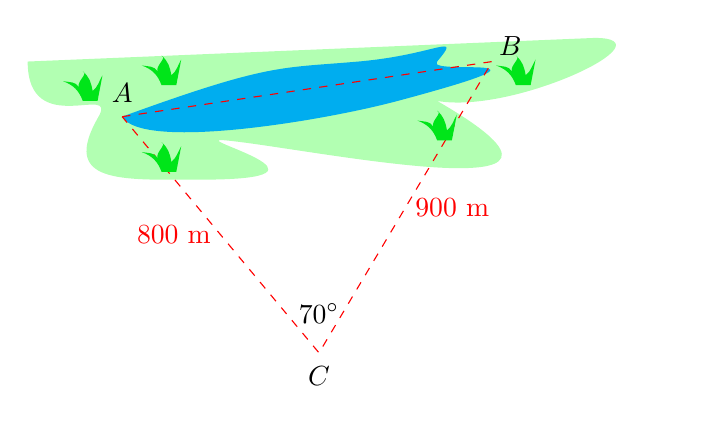
\begin{tikzpicture}
				\tikzset{co/.pic={
						\fill[green!80!teal,out=110,in=-20] (0,0)to(-1,1)[out=-10,in=120]to(-0.2,0.7)[out=110,in=-20]to(0,1.5)[out=-40,in=100]to(0.5,0.5)[out=40,in=-120]to(1,1.3)--(0.75,0)--cycle;
				}}
				\tikzset{Ho/.pic={
						\fill[green!30](-2.2,1.5)--(5,1.8)..controls++(0:1) and++(-10:1)..(3,1)..controls++(-30:3) and++(-5:1)..(0.3,0.5)..controls++(175:0.5) and++(0:2)..(0,0)..controls++(180:1) and++(-120:1)..(-1.3,0.8)..controls++(60:0.5) and++(-90:1)..(-2.2,1.5);
						\fill[cyan](-1,0.8)..controls++(20:2) and++(185:1)..(2,1.5)..controls++(5:1) and++(50:0.5)..(3,1.5)..controls++(-130:0.25)and++(15:2.5)..(2.5,1)..controls++(-165:1) and++(-60:0.5)..(-1,0.8);
						\draw[dashed,red](-1,0.8)coordinate(A)--(3.7,1.5)coordinate(B)--(1.5,-2.2)coordinate(C)node[pos=0.5,right]{$900$ m}--(A)node[pos=0.5,left]{$800$ m};
				}}
				\path(0,0)pic{Ho};
				\foreach \x/\y in{-1.5/1,-0.5/0.1,3/0.5,4/1.2,-0.5/1.2}
				\path(\x,\y)pic[scale=0.25]{co};
				(A)--(B)--(C)--cycle
				\draw	(C)++(90:0.5)node{$70^\circ$};
				\foreach \x/\g in {A/90,B/40,C/-90} \draw (\x)+(\g:0.3)node{$\x$};
			\end{tikzpicture}
		\end{center}
		Theo  định lý côsin, ta có $$AB^2=CA^2+CB^2-2\cdot CA\cdot CB\cdot \cos C=800^2+900^2-2\cdot 800\cdot 900\cdot \cos 70^\circ\approx957491.$$
		Suy ra $AB\approx979$ m.\\
		Vậy khoảng cách giữa hai điểm bờ hồ là  $979$ m
	}
\end{ex}
\begin{ex}%[0H4H3-2]%[Dự án đề cương 3 khối NH24-25 - Đợt 2 - Vũ Ngọc Hào]
	\immini{
		Để đo chiều cao $CH$ của một  tháp truyền thông, người ta chọn hai điểm quan sát $A$, $B$ trên mặt đất (hình vẽ).  Biết $\widehat{CAH}=50^\circ$, $\widehat{CBH}=60^\circ$ và $AB=80$ m. Tính chiều cao của tháp (kết quả làm tròn đến hàng phần mười).
		\choice
		{$300{,}3$ m}
		{\True $305{,}6$ m}
		{$301{,}8$ m}
		{$306{,}9$ m}
	}
	{
		\begin{tikzpicture}[scale=1, font=\footnotesize, line join=round, line cap=round,>=stealth]
			\path
			(1,0) coordinate (A)
			(2,0) coordinate (B)
			(4,3.5) coordinate (C)
			(4,0) coordinate (H)
			;
			\draw [fill=gray!40]
			(3.7,0)
			.. controls ++(50:0.5) and ++(265: 1) .. (C)
			.. controls ++(-85:1) and ++(130: 0.5) .. (4.3,0)--cycle;
			\draw (A)--(C)--(H)--(A) (B)--(C) ;
			\draw pic["$50^{\circ}$", draw=black, angle eccentricity=1.6, angle radius=0.5cm]{angle=H--A--C};
			\draw pic["$60^{\circ}$", draw=black, double, angle eccentricity=1.6, angle radius=0.5cm]{angle=H--B--C};
			\foreach \x/\g in {A/-90,B/-90,C/90,H/-90}
			\fill[black] (\x) circle (1pt)+(\g:3mm) node {$\x$};
		\end{tikzpicture}
	}
	\loigiai{
		Ta có $\widehat{ACB}=\widehat{CBH}= 60^\circ -50^\circ= 10^\circ$. \\
		Áp dụng định lí sin trong $\triangle ABC$ ta có
		\[
		\dfrac{AB}{\sin \widehat{ACB}}=\dfrac{BC}{\sin \widehat{CAH} } \Rightarrow BC=\dfrac{AB\sin \widehat{CAH}}{\sin \widehat{ACB}}=\dfrac{80\sin 50^\circ}{\sin 10^\circ}.
		\]
		Suy ra $CH=BC\sin \widehat{CBH}=\dfrac{80\sin 50^\circ\sin 50^\circ}{\sin 10^\circ} \approx 305{,}6$ m.
	}
\end{ex}
\begin{ex}%[0H4H3-1]%[Dự án đề cương 3 khối NH24-25 - Đợt 2 - Vũ Ngọc Hào]
	Cho tam giác $ABC$ có $AB=16$, $BC=18$, $AC=20$. $M$ là điểm thuộc cạnh $BC$  sao cho $BM=2CM$. Tính góc $\widehat{BAM}$.
	\choice
	{$40{,}5^\circ$}
	{\True $42{,}9^\circ$}
	{$38{,}9^\circ$}
	{$44{,}5^\circ$}
	\loigiai{
		\begin{center}
			\begin{tikzpicture}[scale=1, font=\footnotesize, line join=round, line cap=round,>=stealth]
				\path
				(0,0) coordinate (B)
				(3.5,0) coordinate (C)
				;
				\coordinate (M) at ($(B)!{2/3}!(C)$) ;
				\coordinate (A) at ($(B)+(70:3)$) ;
				\draw (A)--(B)--(C)--(A) (A)--(M) ;
				\foreach \x/\g in {A/90,B/-120,C/-60,M/-90}
				\fill[black] (\x) circle (1pt)+(\g:3mm) node {$\x$};
			\end{tikzpicture}
		\end{center}
		Ta có $BM=2CM \Rightarrow BM=\dfrac{2}{3}BC=12$.\\
		Áp dụng định lí côsin $\triangle ABM$ ta có
		\[
		\cos B=\dfrac{BA^2+BC^2-AC^2}{2 \cdot BA \cdot BC}=\dfrac{16^2+18^2-20^2}{2 \cdot 16 \cdot 18}=\dfrac{5}{16}.
		\]
		Suy ra
		\[
		AM^2=BA^2+BM^2-2BA \cdot BM \cos B=16^2+12^2-2 \cdot 16 \cdot 12 \cdot \dfrac{5}{16}=280 \Rightarrow AM=\sqrt{280}.
		\]
		Áp dụng định lí côsin trong $\triangle AMD$ ta có
		\begin{align*}
			& \cos \widehat{BAM}=\dfrac{AB^2+AM^2- BM^2}{2AB \cdot AM}  \\
			\Leftrightarrow~ & \cos \widehat{BAM}=\dfrac{16^2+280-12^2}{2 \cdot 16 \cdot \sqrt{280}}= \dfrac{7\sqrt{70}}{80}\\
			\Rightarrow~& \widehat{BAM} \approx 42{,}9^\circ.
		\end{align*}
	}
\end{ex}

\begin{ex}%[0H4H3-2]%[Dự án đề cương 3 khối NH24-25 - Đợt 2 - Vũ Ngọc Hào]
	\immini{
		Cho tứ giác $ABCD$ có $AB=35$, $BC=42$, $CD=51$, $\widehat{ABC}=145 ^\circ$, $\widehat{BCD}=98^\circ$. Tính độ dài cạnh $AD$.
		\choice
		{$74{,}2$}
		{$77{,}3$}
		{$71{,}7$}
		{\True $70{,}5$}
	}
	{
		\begin{tikzpicture}[scale=1, font=\footnotesize, line join=round, line cap=round,>=stealth]
			\path
			(0.7,2) coordinate (A)
			(1.9,0.7) coordinate (B)
			(3.8,0) coordinate (C)
			(5,2) coordinate (D)
			;
			\draw  (A)--(B)--(C)--(D)--(A);
			\draw pic["$98^{\circ}$", draw=black, angle eccentricity=1.5, angle radius=0.4cm]{angle=D--C--B} ;
			\draw pic["$145^{\circ}$", draw=black, double, angle eccentricity=1.5, angle radius=0.4cm]{angle=C--B--A};
			\foreach \x/\g in {A/110,B/-120,C/-60,D/60}
			\fill[black] (\x) circle(1.1pt)+(\g:3mm) node {$\x$};
		\end{tikzpicture}
	}
	\loigiai{
		\begin{center}
			\begin{tikzpicture}[scale=1, font=\footnotesize, line join=round, line cap=round,>=stealth]
				\path
				(0.7,2) coordinate (A)
				(1.9,0.7) coordinate (B)
				(3.8,0) coordinate (C)
				(5,2) coordinate (D)
				;
				\coordinate (M) at (intersection of A--B and D--C);
				\draw  (A)--(B)--(C)--(D)--(A);
				\draw [dashed] (B)--(M)--(C) ;
				\draw pic["$98^{\circ}$", draw=black, angle eccentricity=1.5, angle radius=0.4cm]{angle=D--C--B} ;
				\draw pic["$145^{\circ}$", draw=black, double, angle eccentricity=1.5, angle radius=0.4cm]{angle=C--B--A};
				\foreach \x/\g in {A/110,B/-120,C/-60,D/60,M/-90}
				\fill[black] (\x) circle(1.1pt)+(\g:3mm) node {$\x$};
			\end{tikzpicture}
		\end{center}
		Gọi $M$ là giao điểm của $AB$ và $CD$.  \\
		Ta có $\widehat{MBC}=180^\circ-145^\circ=35^\circ$, $\widehat{MCB}=180^\circ-98^\circ=82^\circ$,  $\widehat{BMC}=180^\circ -35^\circ-98^\circ=47^\circ$.\\
		Áp đụng định lí sin
		\begin{align*}
			&\dfrac{BC}{\sin \widehat{BMC}}=\dfrac{CM}{\sin \widehat{MBC}} \Rightarrow CM=\dfrac{BC \sin \widehat{MBC}}{\sin \widehat{BMC}}=\dfrac{42\sin 35^{\circ}}{\sin 47^{\circ}} \Rightarrow MD \approx  83{,}9392; \\
			&\dfrac{BC}{\sin \widehat{BMC}}=\dfrac{BM}{\sin \widehat{MCB}} \Rightarrow BM=\dfrac{BC \sin \widehat{MCB}}{\sin \widehat{BMC}}=\dfrac{42\sin 82^{\circ}}{\sin 47^{\circ}} \Rightarrow MA \approx  91{,}8689.
		\end{align*}
		Áp dụng định lí côsin
		\begin{align*}
			AD &=\sqrt{MA^2+MD^2-2MA\cdot MD \cos \widehat{AMD}} \\
			&= \sqrt{91{,}8689^2+83{,}9392^2-2 \cdot 91{,}8689 \cdot 83{,}93928 \cos 47^\circ}  \\
			&\approx 70{,}5.
		\end{align*}
	}
\end{ex}

\begin{ex}%[0H4V3-2]%[Dự án đề cương 3 khối NH24-25 - Đợt 2 - Vũ Ngọc Hào]
	Từ vị trí $A$ người ta quan sát một cây cao. Biết $AH=4$cm, $HB=20$ m, $\widehat{BAC}=45^{\circ}$. Khi đó chiều cao của cây là (tính chính xác đến hàng phần mười).
	\begin{center}
		\definecolor{lightcornflowerblue}{rgb}{0.6, 0.81, 0.93}
		\definecolor{cadmiumgreen}{rgb}{0.0, 0.42, 0.24}
		\definecolor{trueblue}{rgb}{0.0, 0.45, 0.81}
		\definecolor{tumbleweed}{rgb}{0.87, 0.67, 0.53}%màu cát
		
		\definecolor{forestgreen(web)}{rgb}{0.13, 0.55, 0.13}
		\definecolor{darkpastelgreen}{rgb}{0.01, 0.75, 0.24}
		\definecolor{bronze}{rgb}{0.8, 0.5, 0.2}
		\begin{tikzpicture}[line join=round, line cap=round,scale=1.5,transform shape]
			\clip (-4,-2.5) rectangle (4,2.5);
			\tikzset{cay/.pic={
					\def\T{ %Thân
						(-.33,0)%trái
						..controls +(-50:.25) and +(40:.45) ..  (-.57,-1.45)
						..controls +(20:.1) and +(-160:.15) ..  (-.1,-1.3)
						..controls +(-120:.1) and +(60:.15) ..  (-.2,-1.6)
						..controls +(-30:.1) and +(-140:.15) ..  (.15,-1.3)
						..controls +(-20:.1) and +(-160:.15) ..  (.57,-1.4)
						..controls +(170:.4) and +(-160:.1) ..  (.35,0)
						..controls +(110:.5) and +(80:.5) ..  (-.33,0)
						;}
					%\draw \T;
					\fill[bronze] \T;
					\def\C{ 
						(0,.3)
						..controls +(-100:.25) and +(-60:.2) ..  (-.3,.1)
						..controls +(-100:.25) and +(-60:.2) ..  (-.6,0)
						..controls +(-120:.45) and +(-110:.35) ..  (-1,.2)
						..controls +(-150:.5) and +(-140:.35) ..  (-1.15,.7)%nút giao
						..controls +(-170:.4) and +(-170:.35) ..  (-1,1.15)
						..controls +(140:.35) and +(110:.4) ..  (-.37,1.35)
						..controls +(110:.25) and +(80:.3) ..  (-.15,1.35)
						..controls +(80:.3) and +(95:.8) ..  (.55,1.1)
						..controls +(80:.2) and +(95:.2) ..  (.8,1.1)
						..controls +(20:.1) and +(95:.1) ..  (.95,1)
						..controls +(-20:.4) and +(35:.25) ..  (1,.47)
						..controls +(-30:.3) and +(-20:.3) ..  (.75,0.05)%nút giao
						..controls +(-120:.3) and +(-60:.2) ..  (.35,0)
						..controls +(175:.2) and +(-160:.1) ..  (.2,0.2)
						..controls +(-160:.1) and +(-70:.1) ..  (0,.3)
						;}
					\draw \C;
					\fill[forestgreen(web)] \C;
					\def\C1{ 
						(-1.15,.7)%nút giao
						..controls +(-170:.4) and +(-170:.35) ..  (-1,1.15)
						..controls +(140:.35) and +(110:.4) ..  (-.37,1.35)
						..controls +(110:.25) and +(80:.3) ..  (-.15,1.35)
						..controls +(80:.3) and +(95:.8) ..  (.55,1.1)
						..controls +(80:.2) and +(95:.2) ..  (.8,1.1)
						..controls +(20:.1) and +(95:.1) ..  (.95,1)
						..controls +(-20:.4) and +(35:.25) ..  (1,.47)
						..controls +(-50:.5) and +(-85:.6) ..  (.65,.55)% gần nút giao
						..controls +(-160:.4) and +(-120:.4) ..  (0,.7)
						..controls +(-150:.2) and +(-80:.4) ..  (-.63,.6)
						..controls +(-140:.5) and +(-130:.4) ..  (-1.15,.7)
						;}
					%\draw \C1;
					\fill[darkpastelgreen] \C1;
					\def\G{ %Gân
						(-.8,.2)
						..controls +(-35:.1) and +(130:.35) ..  
						(-.32,0)%nút giao
						..controls +(-40:.1) and +(45:.35) ..  (-.42,-1.25)
						(-.32,0)%nút giao
						..controls +(120:.1) and +(-45:.35) ..  (-.58,.45)
						(-.32,0)%nút giao
						..controls +(80:.1) and +(-170:.35) ..  (-.05,.45)
						(-.28,.3)
						..controls +(80:.1) and +(-60:.05) ..  (-.35,.55)
						%Gân phải
						(.45,-1.3)
						..controls +(130:.6) and +(-160:.3) ..  (.6,0.35)
						(.37,0)
						..controls +(35:.2) and +(-150:.1) ..  (.66,0.15)
						(.37,0)
						..controls +(80:.2) and +(-40:.1) ..  (.18,0.4)
						(.31,0.25)
						..controls +(80:.1) and +(-150:.1) ..  (.38,0.5)
						(.25,-0.15)
						..controls +(-110:.05) and +(110:.05) ..  (.2,-0.5)%gân dọc
						(.2,-0.25)
						..controls +(-110:.05) and +(110:.05) ..  (.17,-0.45)
						(-.2,-0.15)
						..controls +(-70:.1) and +(110:.05) ..  (-.18,-0.5)
						(-.15,-0.15)
						..controls +(-70:.1) and +(110:.05) ..  (-.15,-0.7)
						(-.05,-0.8)
						..controls +(-80:.15) and +(-10:.15) ..  (-.3,-1.28)
						(-.1,-0.9)
						..controls +(-110:.1) and +(20:.05) ..  (-.2,-1.1)
						(.1,-1)
						..controls +(-50:.05) and +(120:.05) ..  (.15,-1.2)
						(.1,-1.15)
						..controls +(-50:.05) and +(120:.05) ..  (.12,-1.2)
						(.15,-.75)
						..controls +(-120:.1) and +(-140:.1) ..  (.22,-.9)
						..controls +(70:.12) and +(120:.05) ..  (.18,-.9)
						;}
					
					\draw \G;
					
			}}
			
			\path
			(2,0)pic[scale=.8]{cay}	;
			\path 	(2,-1.1) coordinate (B)
			(-2,-1.1) coordinate (H)
			(-2,-.5) coordinate (A)
			(2,1.25) coordinate (C)	;
			\node at (B) [below]{\tiny $B$};
			\node at (H) [below]{\tiny $H$};
			\node at (A) [left]{\tiny $A$};
			\node at (C) [above]{\tiny $C$};
			\node at (-2,-.8) [left]{\tiny $4$};
			\node at (0,-1.1) [below]{\tiny $20$};
			\draw (B)--(H)--(A)--(C) (A)--(B);
			\draw    pic["\tiny $45^\circ$", draw=black, angle eccentricity=1.8, mark=1,angle radius=.4cm, color=blue]
			{angle=B--A--C};
			\draw    pic[draw=black, angle radius=.1cm]
			{right angle=A--H--B}; 
		\end{tikzpicture}
	\end{center}
	\choice
{\True $ 17{,}3$ m}
{$ 17{,}6$ m}
{$ 17{,}9$ m}
{$ 17$ m}
	\loigiai{
		Tam giác $ AHB $ vuông tại $ H $ nên ta có $ AB=\sqrt{AH^2+HB^2}=\sqrt{4^2+20^2}=4\sqrt{26}$ m.\\
		Ta có $ \tan \widehat{HAB}=\dfrac{BH}{AH}=5\Rightarrow \widehat{HAB}\approx 78{,}7^\circ$.\\
		Ta lại có $ AH \parallel BC \Rightarrow \widehat{ABC}=\widehat{HAB}\approx 78{,}7^\circ\Rightarrow \widehat{ACB}=180^\circ-\widehat{CAB}-\widehat{ABC}\approx 56{,}3^\circ $.\\
		Áp dụng định lý sin trong tam giác $ ABC $ ta có \\
		$\dfrac{BC}{\sin\widehat{BAC}}=\dfrac{AB}{\sin\widehat{ACB}}\Rightarrow BC=\dfrac{AB}{\sin\widehat{ACB}}\cdot \sin\widehat{BAC}\approx 17{,}3$\,m.
	}
\end{ex}

\Closesolutionfile{ans}

\ind{PHẦN II.} \inden{Câu trắc nghiệm đúng sai. Trong mỗi ý a), b), c), d) ở mỗi câu, học sinh chọn đúng hoặc sai.}\\
\setcounter{ex}{0}
\Opensolutionfile{ans}[ans/0H4-Bai3-DS]%--Đặt tên 2D1-Bai1-DS
\begin{ex}[Trích đề kiểm tra Toán 10 GHKI THPT Chuyên Lê Quý Đôn Ninh Thuận NH24-25]%[0H4H3-1]%[Dự án đề cương 3 khối NH24-25 - Đợt 2 - Vũ Ngọc Hào]
	Cho tam giác $ABC$ có các cạnh $AB=8$, $AC=5$, $\widehat{A}=60^\circ$.
	\choiceTF
	{\True Diện tích tam giác $ABC$ bằng $10\sqrt{3}$}
	{Độ dài cạnh $BC$ bằng $6$}
	{Bán kính đường tròn nội tiếp tam giác $ABC$ là $r=\sqrt{3}$}
	{\True Khoảng cách từ $B$ đến $AC$ bằng $4\sqrt{3}$}
	\loigiai{
		\begin{itemchoice}
			\itemch Diện tích tam giác $ABC$ được tính bằng
			\[S=\dfrac{1}{2}AB\cdot AC\cdot \sin \widehat{A}=\dfrac{1}{2}\cdot 8\cdot 5\cdot \sin 60^\circ=10\sqrt{3}.\]
			\itemch Áp dụng định lý cô-sin trong tam giác $ABC$ ta có
			\[BC^2=AB^2+AC^2-2AB\cdot AC\cdot \cos \widehat{A}=8^2+5^2-2\cdot 8\cdot 5\cdot \cos 60^\circ=49.\]
			Vậy $BC=7$.
			\itemch Bán kính đường tròn nội tiếp tam giác $ABC$ được tính bằng
			\[r=\dfrac{S}{p}=\dfrac{10\sqrt{3}}{\dfrac{8+5+6}{2}}=\dfrac{10\sqrt{3}}{\dfrac{19}{2}}=\dfrac{20\sqrt{3}}{19}.\]
			\itemch Khoảng cách từ $B$ đến $AC$ được tính bằng
			\[h=\dfrac{2S}{AC}=\dfrac{2\cdot 10\sqrt{3}}{5}=4\sqrt{3}.\]
		\end{itemchoice}
	}
\end{ex}
\begin{ex}[Trích đề kiểm tra Toán 11 GHKI THPT Chuyên Lê Quý Đôn Ninh Thuận NH24-25]%[0H4H2-1]%[Dự án đề cương 3 khối NH24-25 - Đợt 2 - Vũ Ngọc Hào]
	Cho tam giác $ABC$ có $\widehat{C}=60^{\circ}$, $b=10$, $a=20$.
	\choiceTF
	{\True Độ dài cạnh còn lại của tam giác $ABC$ là $c=10 \sqrt{3}$}
	{\True Bán kính đường tròn ngoại tiếp tam giác $ABC$ là $R=10$}
	{\True Độ dài đường trung tuyến hạ từ đỉnh $A$ của tam giác $ABC$ là $m_a=10$}
	{Độ dài đường cao hạ từ đỉnh $A$ của tam giác $ABC$ là $h_a=10 \sqrt{3}$}
	\loigiai{
		\begin{center}
			\begin{tikzpicture}[scale=.9, font=\footnotesize, line join=round, line cap=round, >=stealth]
				\coordinate[label=left:$C$] (C) at (0,0);
				\coordinate[label=right:$B$] (B) at ($(C)+(6,0)$);
				\coordinate[label=above:$A$, shift=(60:4cm)] (A) at (C);
				\coordinate[label=below:$M$]  (M) at ($(B)!1/2!(C)$);
				\coordinate[label=below:$H$] (H) at ($(B)!(A)!(C)$);
				\draw[line width=0.4pt,black] (A)--(M)node[right,pos=0.5]{$ m_a $};
				\draw[line width=0.4pt,black] (A)--(H)node[left,pos=0.5]{$ h_a $};
				\draw (A)--(B)--(C)--cycle;
				\draw pic [draw, angle radius=9 mm] {angle=B--C--A};
				\foreach \x in {A,B,C,M,H} \fill[black] (\x) circle (1.5pt);
			\end{tikzpicture}
		\end{center}
		\begin{itemchoice}
			\itemch Theo định lý cos, ta có $ c=\sqrt{a^2+b^2-2ab\cos C}=10\sqrt{3} $.
			\itemch Theo đính lý sin, ta có $ R=\dfrac{c}{2\sin C}=\dfrac{10\sqrt{3}}{2\sin 60^\circ}= 10$.
			\itemch Gọi $ M $ là trung điểm $ BC $ nên $BM=MC=\dfrac{BC}{2}=10 $.\\
			Ta có $m_a=MA=\sqrt{10^2+10^2-2\cdot 10\cdot 10 \cdot \cos 60^\circ}=10 $.
			\itemch  Ta có $ S_{ABC}=\dfrac{1}{2}ba\sin C=50\sqrt{3}$.\\
			Gọi $ H $ là chân đường cao hạ từ $A$ của $\triangle ABC$.\\
			Ta có $ S_{ABC}=\dfrac{1}{2}\cdot AH\cdot BC \Leftrightarrow h_a=HA=\dfrac{2S_{ABC}}{BC}=\dfrac{2\cdot 50\sqrt{3}}{20}= 5\sqrt{3}$.
		\end{itemchoice}
	}
\end{ex}
\begin{ex}%[0H4H3-1]%[Dự án đề cương 3 khối NH24-25 - Đợt 2 - Vũ Ngọc Hào]
	Cho tam giác $ABC$ có $AB=3$, $AC=2$, $\widehat{A}=60^\circ$. Trên cạnh $BC$ lấy điểm $M$ nằm giữa $B$ và $C$.
	\choiceTF
	{$BC^2=AB^2+AC^2+2 AB\cdot AC\cdot\cos A$}
	{\True $BC=\sqrt{7}$}
	{$\cos B=\dfrac{\sqrt{7}}{7}$}
	{Độ dài $AM$ nhỏ nhất bằng $\dfrac{189}{49}$}
	\loigiai{
		\begin{itemchoice}
			\itemch  Ta có $BC^2=AB^2+AC^2-2 AB\cdot AC\cdot\cos A$
			\itemch $$BC^2=AB^2+AC^2-2 AB\cdot AC\cdot\cos A=9+4-2\cdot 3\cdot 2\cdot\cos 60^\circ=7\Rightarrow BC=\sqrt{7}.$$
			\itemch  Ta có $\cos B=\dfrac{AB^2+BC^2-AC^2}{2\cdot AB\cdot BC}=\dfrac{9+7-4}{2\cdot 3\cdot\sqrt{7}}=\dfrac{2\sqrt{7}}{7}$.
			\itemch  Với $M$ tùy ý nằm giữa $B$ và $C$ ,ta có
			\begin{eqnarray*}
				AM^2&=&AB^2+BM^2-2 AB\cdot BM\cdot\cos B=9+BM^2-2\cdot 3\cdot BM\cdot\dfrac{2\sqrt{7}}{7}\\
				&=&BM^2-\dfrac{12\sqrt{7}}{7} BM+9\\
				&=&\left(BM-\dfrac{6\sqrt{7}}{7}\right)^2+\dfrac{189}{49}\geq\dfrac{189}{49}.
			\end{eqnarray*}
			Do đó $AM^2\geq\dfrac{189}{49}\Rightarrow AM\geq\dfrac{\sqrt{189}}{7}$.\\
			Dấu bằng xảy ra khi $BM-\dfrac{6\sqrt{7}}{7}=0\Leftrightarrow BM=\dfrac{6\sqrt{7}}{7}$ hay $BM=\dfrac{6}{7}BC$.
		\end{itemchoice}
	}
\end{ex}

\begin{ex}%[0H4V3-2]%[Dự án đề cương 3 khối NH24-25 - Đợt 2 - Vũ Ngọc Hào]
	Lúc $7$ giờ kém $5$ sáng,bạn Mai đi xe đạp tự nhà (điểm $A$) đến trường (điểm $B$) phải đi lên dốc và xuống một con dốc (hình vẽ). Cho biết đoạn lên dốc dài $300$ m, $A=6^\circ $, $B=4^\circ$. Gọi $C$ là đỉnh dốc.
	\begin{center}
		\begin{tikzpicture}[font=\footnotesize, line join=round, line cap=round, >=stealth]
			\path
			(0,0) coordinate (A)
			(7,0) coordinate (B)
			($(A)!1pt!6:(B)$) coordinate (a)
			($(B)!1pt!-4:(A)$) coordinate (b)
			(intersection of A--a and B--b) coordinate (C)
			($(A)!(C)!(B)$) coordinate (H)
			;
			\draw (C)--(A)--(B)--(C)--(H);
			\foreach \x/\y in {A/190, C/90, B/-10,H/-90}
			\draw [fill=black] (\x) circle (0.03cm)+(\y:0.3cm) node {$\x$};
		\end{tikzpicture}
	\end{center}
	\choiceTF
	{\True Độ dốc lúc lên cao hơn lúc xuống}
	{Độ cao con dốc là (làm tròn đến hàng phần mười) là $31{,}3$ m}
	{Quãng đường chim bay đi từ nhà đến trường (làm tròn đến hàng đơn vị) là $749$ m}
	{\True Để kịp đến trường lúc $7$h đúng, Mai đã lên dốc với vận tốc (làm tròn đến hàng đơn vị) là $6$ km/h, biết Mai khi xuống dốc bạn đi tự do không đạp xe với vận tốc không đổi là $15$ km/h}
	\loigiai{
		\begin{itemchoice}
			\itemch Do $A>B$ nên độ dốc lúc lên cao hơn lúc xuống.
			\itemch  Áp dụng hệ thức lượng trong tam giác vuông $ACH$, ta có độ cao con dốc là $$CH=AC\cdot\sin A=300\cdot\sin 6^{0}\approx 31,4~(\mathrm{m}).$$
			\itemch  Xét tam giác $ABC$ có $\widehat{ACB}=180^\circ-4^\circ-6^\circ=170^\circ$.\\
			Áp dụng định lý $\sin$ ta có $\dfrac{AC}{\sin B}=\dfrac{AB}{\sin C}\Rightarrow AB=\dfrac{AC\cdot\sin C}{\sin B}\approx 747$ (m).
			\itemch Sử dụng định lý sin ta có $\dfrac{BC}{\sin A}=\dfrac{AC}{\sin B}\Rightarrow BC=\dfrac{AC\cdot\sin A}{\sin B}\approx 449{,}5$ (m).\\
			Thời gian bạn Mai đi từ nhà tới trường
			$$\dfrac{5}{60}=\dfrac{1}{12}=\dfrac{A C}{v_{A C}}+\dfrac{B C}{15}\Rightarrow v_{A C}=A C:\left(\dfrac{1}{12}-\dfrac{B C}{15}\right)=0{,}3:\left(\dfrac{1}{12}-\dfrac{0{,}3\cdot\sin 6^\circ}{15\cdot\sin 4^\circ}\right)\approx 6~(\mathrm{km}/\mathrm{h}).$$
		\end{itemchoice}
	}
\end{ex}

\begin{ex}%[0H4V3-2]%[Dự án đề cương 3 khối NH24-25 - Đợt 2 - Vũ Ngọc Hào]
	Một đoạn đường đi từ điểm $A$ đến điểm $B$ nhưng bị vướng một ngọn núi. Nhà đầu tư thực hiện phương án xây dựng đường tránh từ $A$ đến $M$, từ $M$ đến $N$ và sau đó mới đến $B$. Biết rằng $AM=3{,}2$ km, $MN=5{,}5$ km, $NB=3{,}6$ km, $\alpha=140^\circ$ và $\beta=145^\circ$.
	\begin{center}
		\begin{tikzpicture}[scale=1, font=\footnotesize, line join=round, line cap=round, >=stealth]
			\path
			(0,0.3) coordinate (A)
			(4.5,0.3) coordinate (B)
			(0.7,-1.2) coordinate (M)
			(2.8,-1.4) coordinate (N)
			;
			\draw
			(A)--(B)--(N)--(A)--(M)--(B)
			(M)--(N)
			;
			\draw 
			pic[draw, angle radius=2mm]{angle=N--M--A}
			pic[draw,double, angle radius=2mm]{angle=B--N--M}
			($(M)+(0.,0.1)$)node[above right]{$\alpha$}
			($(N)+(0.,0.1)$)node[above]{$\beta$}
			;
			\fill[gray!90] (0.5,-0.2)--(1,1.0)--(1.8,1.5)--(2.4,0.5)--(2.6,1.3)--(3,1.5)--(3.4,1)--(3.9,-0.2)--(2.3,-0.5)--(1,-0.6)--cycle ;
			\foreach \x/\g in{A/180, B/0, N/-90, M/-90} \draw[fill=black](\x) circle (1pt)
			($(\x)+(\g:3mm)$) node{\x};
		\end{tikzpicture}
	\end{center}
	\choiceTF
	{\True Số đo của góc $\widehat{ANM}$ bé hơn $15^\circ$}
	{\True Độ dài cạnh $MB\approx 8{,}7$ km (làm tròn đến hàng phần mười)}
	{Độ dài cạnh $AN\approx 3{,}68$ km (kết quả làm tròn đến hàng phần trăm)}
	{\True Giả sử nhà đầu tư dự định phương án đường hầm xuyên qua núi đi thẳng từ $A$ đến $B$ (chi phí cao và sẽ có thu phí). Một người đi xe với vận tốc trung bình $80$ km/h trong đường hầm và vận tốc trung bình $40$ km/h trên đường tránh. Thời gian đi từ $A$ đến $B$ bằng đường hầm sẽ tiết kiệm một khoảng thời gian khoảng $10$ phút (làm tròn hàng đơn vị phút)}
	\loigiai{\begin{center}
			\begin{tikzpicture}[scale=1, font=\footnotesize, line join=round, line cap=round, >=stealth]
				\path
				(0,0) coordinate (A)
				(4.5,0) coordinate (B)
				(0.7,-1.2) coordinate (M)
				(2.8,-1.4) coordinate (N)
				;
				\draw
				(A)--(B)--(N)--(A)--(M)--(B)
				(M)--(N)
				;
				\draw 
				pic[draw, angle radius=2mm]{angle=N--M--A}
				pic[draw,double, angle radius=2mm]{angle=B--N--M}
				($(M)+(0.,0.1)$)node[above right]{$\alpha$}
				($(N)+(0.,0.1)$)node[above]{$\beta$}
				;
				\foreach \x/\g in{A/180, B/0, N/-90, M/-90} \draw[fill=black](\x) circle (1pt)
				($(\x)+(\g:3mm)$) node{\x};
			\end{tikzpicture}
		\end{center}
		\begin{itemchoice}
			\itemch Áp dụng định lý côsin cho tam giác $AMN$ ta được\\
			$\begin{aligned} AN^2&=AM^2+MN^2-2\cdot AM\cdot MN\cdot\cos\widehat{AMN}\\
				&=3{,}2^2+5{,}5^2-2\cdot 3{,}2\cdot5{,}5\cdot\cos140^\circ\approx67{,}455.\\
				\Rightarrow AN&\approx 8{,}213~\mathrm{(km)}.\end{aligned}$\\
			Suy ra $\cos\widehat{ANM}=\dfrac{AN^2+MN^2-AM^2}{2\cdot AN\cdot MN}=\dfrac{8{,}213^2+5{,}5^2-3{,}2^2}{2\cdot8{,}213\cdot5{,}5}\approx0{,}9681$.\\
			$\Rightarrow \widehat{ANM}\approx 14^\circ30'$.
			\itemch	Áp dụng định lý côsin cho tam giác $BMN$ ta được\\
			$\begin{aligned} MB^2&=NM^2+NB^2-2\cdot NM\cdot NB\cdot\cos\widehat{MNB}\\
				&=5{,}5^2+3{,}6^2-2\cdot 5{,}5\cdot3{,}6\cdot\cos145^\circ\approx75{,}648.\\
				\Rightarrow MB&\approx 8{,}7~\mathrm{(km)}.\end{aligned}$
			\itemch	Ta có $AN\approx 8{,}21$ (km).
			\itemch Ta có $\widehat{ANB}=145^\circ-\widehat{ANM}\approx 145^\circ-14^\circ30'\approx 130^\circ30'$.\\
			Áp dụng định lý côsin cho tam giác $ANB$ ta được\\
			$\begin{aligned} AB^2&=AN^2+NB^2-2\cdot AN\cdot NB\cdot\cos\widehat{ANB}\\
				&\approx 8{,}213^2+3{,}6^2-2\cdot 8{,}213\cdot3{,}6\cdot\cos\left(130^\circ30'\right)\approx118{,}82.\\
				\Rightarrow AB&\approx 10{,}9~\mathrm{(km)}.\end{aligned}$\\
			Thời gian đi xe trong đường hầm là $\dfrac{10{,}9}{80}=\dfrac{109}{800}$ (giờ) $=\dfrac{327}{40}$ (phút).\\
			Thời gian đi xe trên đường tránh là $\dfrac{3{,}2+5{,}5+3{,}6}{40}=\dfrac{123}{400}$ (giờ) $=\dfrac{369}{20}$ (phút).\\
			Suy ra thời gian từ $A$ đến $B$ sẽ tiết kiệm một khoảng thời gian khoảng\break $\dfrac{369}{20}-\dfrac{327}{40}=\dfrac{411}{40}\approx 10$ phút.
		\end{itemchoice}
	}
\end{ex}
\Closesolutionfile{ans}

\ind{PHẦN III.} \inden{Câu trắc nghiệm trả lời ngắn.}
%\inden{Câu trắc nghiệm đúng sai. Trong mỗi ý a), b), c), d) ở mỗi câu, học sinh chọn đúng hoặc sai.}\\
\setcounter{ex}{0}
\Opensolutionfile{ans}[ans/0H4-Bai3-DS]%--Đặt tên 2D1-Bai1-DS
\begin{ex}[Trích đề kiểm tra Toán khối 10 HK1 NH24-25-Chuyên Lê Quý Đôn-Nình Thuận]%[0H4H3-2]%[Dự án đề cương 3 khối NH24-25 - Đợt 2 - Vũ Ngọc Hào]
	Từ một miếng bìa hình tròn, bạn Nam cắt ra một hình tam giác có độ dài ba cạnh tương ứng là $4$ cm, $5$ cm, $6$ cm và các đỉnh của tam giác là các điểm thuộc viền của miếng bìa. Tính bán kính của miếng bìa ban đầu (làm tròn kết quả đến hàng phần trăm theo đơn vị xăng-ti-mét).
	\shortans[oly]{$7{,}76$}
	\loigiai{
		\immini{
			Gọi tam giác $ABC$ là tam giác có độ dài ba cạnh tương ứng là $4$ cm, $5$ cm, $6$ cm và các đỉnh của tam giác là các điểm thuộc viền của miếng bìa hình tròn.\\
			Áp dụng định lí côsin vào $\triangle ABC$ có
			\allowdisplaybreaks
			\begin{eqnarray*}
				\cos A=\dfrac{AB^2+AC^2-BC^2}{2AB\cdot AC}=\dfrac{6^2+4^2-5^2}{2\cdot 6\cdot 4}=\dfrac{9}{16}.
			\end{eqnarray*}
			Khi đó $\sin A=\sqrt{1-\cos^2 A}=\dfrac{5\sqrt{7}}{16}$.\\
			Áp dụng định lí sin vào $\triangle ABC$ có
			\begin{eqnarray*}
				\dfrac{BC}{\sin A}=2R\Rightarrow R=\dfrac{2BC}{\sin A}=\dfrac{2\cdot 6}{\dfrac{5\sqrt{7}}{16}}\approx 7{,}76\,\text{cm}.
			\end{eqnarray*}
		}{
			\begin{tikzpicture}[scale=0.7,font=\footnotesize,line join=round,line cap=round,>=stealth]
				\path 
				(0,0) coordinate (O)
				(60:2.5) coordinate (A)
				(-30:2.5) coordinate (C)
				(-150:2.5) coordinate (B)
				;
				\draw (A)--(B)--(C)--(A)--(O)--(B) (O)--(C) (O) circle (2.5);
				
				\foreach \x/\g in {A/90,B/180,C/-45,O/120}
				\fill[black] 	(\x) circle (1pt)
				($(\g:3mm)+(\x)$) node {$\x$};
			\end{tikzpicture}
		}
	}
\end{ex}

\begin{ex}%[0H4H3-2]%[Dự án đề cương 3 khối NH24-25 - Đợt 2 - Vũ Ngọc Hào]
	\immini{
		Để đo khoảng cách từ $A$ đến $B$ ngang qua một cái hồ nước, người ta chọn điểm  $C$, sau đó đo độ dài các cạnh $AC$, $BC$ và góc $C$.  Biết $AC=112$ m, $BC=145$ m, $\widehat{C}=75^\circ$, khoảng cách từ $A$ đến $B$ gần bằng bao nhiêu mét (làm tròn đến hàng đơn vị)?
		\shortans[oly]{$159$}
	}
	{
		\begin{tikzpicture}[scale=1, font=\footnotesize, line join=round, line cap=round,>=stealth]
			\path
			(2,2) coordinate (A)
			(7,2) coordinate (B)
			(2.5,2) coordinate (D)
			(3.5,3.1) coordinate (E)
			(5.5,2.9) coordinate (F)
			(6.4,1.5) coordinate (G)
			(5.2,0.7) coordinate (H)
			(3.5,0.7) coordinate (I)
			(2.6,1.3) coordinate (J)
			;
			\coordinate (C) at ($(A)+(53.6:3.6)$) ;
			\draw[fill=cyan!40]
			(D)
			.. controls ++(65:0.1) and ++(200: 1) .. (E)
			.. controls ++(200:-0.5) and ++(170: 0.3) .. (F)
			.. controls ++(170:-0.5) and ++(100: 0.3) .. (G)
			.. controls ++(100:-0.3) and ++(30: 0.3) .. (H)
			.. controls ++(30:-0.3) and ++(150: -0.3) .. (I)
			.. controls ++(150:0.3) and ++(130: -0.3) .. (J)
			.. controls ++(130:0.3) and ++(65: -0.1) .. (D)
			;
			\draw[dashed] (D)--(6.2,2) ;
			\draw (A)--(C)--(B)  (A)--(D) (B)--(6.2,2) ;
			\draw pic["$75^{\circ}$", draw=black, angle eccentricity=1.4, angle radius=0.5cm]{angle=A--C--B};
			\foreach \x/\g in {A/-120,B/-60,C/90}
			\fill[black] (\x) circle (1pt)+(\g:3mm) node {$\x$};
		\end{tikzpicture}
	}
	\loigiai{
		Áp dụng định lí côsin ta có
		\begin{align*}
			AB^2=AC^2+BC^2-2AC \cdot BC \cos C=112^2+145^2-2 \cdot 112 \cdot 145 \cos 75^\circ  \Rightarrow AB \approx 158{,}6 \mathrm{~(m).}
		\end{align*}
	}
\end{ex}
\begin{ex}%[0H4V3-2]%[Dự án đề cương 3 khối NH24-25 - Đợt 2 - Vũ Ngọc Hào]
	\immini{Nhà bạn Bình và nhà bạn Cẩn ở hai vị trí $P$ và $Q$ cách nhau $53$ m thẳng hàng với chân $A$ của tòa nhà Vinhomes Park. Từ nhà Bình và nhà Cẩn lần lượt nhìn đỉnh $B$ của tháp với góc $59^\circ$ và $72^\circ$ (như hình vẽ bên). Hỏi chiều cao $AB$ của tháp bằng bao nhiêu mét (làm tròn đến hàng đơn vị)?
		\shortans[oly]{$192$}
	}{
		\begin{tikzpicture}[scale=1, font=\footnotesize, line join=round, line cap=round,>=stealth]
			\path
			(1,0) coordinate (P)
			(2.5,0) coordinate (Q)
			(4,3.5) coordinate (B)
			(4,0) coordinate (A)
			;
			\draw [fill=red!30]
			(3.7,0)
			.. controls ++(50:0.5) and ++(265: 1) .. (B)
			.. controls ++(-85:1) and ++(130: 0.5) .. (4.3,0)--cycle;
			\draw (P)--(B)--(A)--(P)--(Q)node[pos=0.5,below]{$53\,\text{m}$}--(B) ;
			\foreach \x/\g in{P/180,Q/-60, B/180, A/-90}
			\fill[black] (\x) circle (1pt)+(\g:3mm) node {$\x$};
			\draw[-] ($(P)!4mm!(A)$) to[bend right=60] node[pos=.7,right]{$59^\circ$} ($(P)!4mm!(B)$);
			\draw[dashed] ($(Q)!4mm!(A)$) to[bend right=60] node[pos=.7,right]{$72^\circ$} ($(Q)!4mm!(B)$);
		\end{tikzpicture}
	}
	\loigiai{ Từ hình vẽ ta có $\widehat{PQB}=180^\circ-72^\circ=108^\circ$,  $\widehat{PBQ}=180^\circ-59^\circ-108^\circ=13^\circ$.\\
		Trong tam giác $PBQ$ có
		\[\dfrac{BQ}{\sin 59^\circ}=\dfrac{PQ}{\sin 13^\circ}\Rightarrow BQ=\dfrac{PQ}{\sin 13^\circ}\cdot \sin 59^\circ=\dfrac{53}{\sin 13^\circ}\cdot \sin 59^\circ \approx 201{,} 95 \ \text{m}.\]
		Trong tam giác $ABQ$ có $AB=BQ\cdot \sin 72^\circ=201{,} 95\cdot \sin 72^\circ \approx 192{,} 07$ m.
	}
\end{ex}

\begin{ex}%[0H4V3-2]%[Dự án đề cương 3 khối NH24-25 - Đợt 2 - Vũ Ngọc Hào]
	\immini{
		Để xác định bán kính của một cái cầu vòm, người ta lấy 3 điểm trên  cầu (hình vẽ) và tiến hành đo. Biết $AB=5{,}8$ m, $BC=9{,}2$ m, $AC=12{,}9$ m. Tính bán kính của cầu (làm tròn đến hàng phần mười).
		\shortans[oly]{$7{,}2$}
	}
	{
		\begin{tikzpicture}[scale=1, font=\footnotesize, line join=round, line cap=round,>=stealth]
			\coordinate (O) at (0,-1);
			\coordinate (A) at ($(O)+(145:3)$) ;
			\coordinate (B) at ($(O)+(107:3)$) ;
			\coordinate (C) at ($(O)+(46:3)$) ;
			\coordinate (D) at ($(O)+(160:3)$) ;
			\coordinate (E) at ($(O)+(20:3)$) ;
			\coordinate (P) at ($(O)+(165:5)$) ;
			\coordinate (Q) at ($(O)+(14.5:4)$) ;
			\draw[pattern=bricks,pattern color=brown]
			(E)--plot[samples=100,smooth,domain=14.5:165]({4*cos(\x)},{-1+4*sin(\x)})--(D) -- plot[samples=100,smooth,domain=160.5:19.5]({3*cos(\x)},{-1+3*sin(\x)});
			\draw (A)--(B)--(C)--(A);
			\draw  (E) arc (20:160:3);
			\foreach \x/\g in {A/-80,B/-90,C/-110}
			\fill[black] (\x) circle (1.1pt)+(\g:3mm) node {$\x$};
		\end{tikzpicture}
	}
	\loigiai{
		Áp dụng định lí côsin ta có
		\begin{eqnarray*}
			&&BC^2=AB^2+AC^2-2AB \cdot AC \cos A  \\
			&\Leftrightarrow & \cos A=\dfrac{AB^2+AC^2- BC^2}{2AB \cdot AC}  \\
			&\Leftrightarrow & \cos A=\dfrac{5{,}8^2+12{,}9^2-9{,}2^2}{2 \cdot 5{,}8 \cdot 12{,}9}\\
			&\Rightarrow & \widehat{A} \approx 39{,}5336^\circ.
		\end{eqnarray*}
		Áp dụng định lí sin suy ra bán kính của chiếc đĩa là
		$R=\dfrac{BC}{2\sin A}=\dfrac{9,2}{2\sin 39{,}5336^\circ} \approx 7{,}2$m.
	}
\end{ex}
\begin{ex}%[0H4V3-2]%[Dự án đề cương 3 khối NH24-25 - Đợt 2 - Vũ Ngọc Hào]
	Quan sát cây cầu dây văng minh hoạ ở (Hình 25). Tại trụ cao nhất, khoảng cách từ đỉnh trụ (vị trí $A$) tới chân trụ trên mặt cầu (vị trí $H$) là $150$ m, độ dài dây văng dài nhất nối từ đỉnh trụ xuống mặt cầu (vị trí $B$) là $300$ m, khoảng cách từ chân dây văng dài nhất tới chân trụ trên mặt cầu là $250$ m (Hình 26). Tính độ dốc của cầu qua trụ nói trên (làm tròn kết quả đến hàng phần mười theo đơn vị độ).
	\shortans[oly]{$3{,}8^{\circ}$}
	\begin{center}
		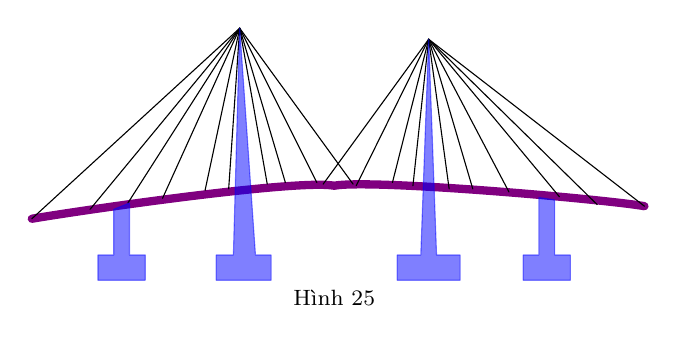
\begin{tikzpicture}[scale=1,>=stealth, font=\footnotesize, line join=round, line cap=round]
			\draw[line width=3pt,violet]
			(-3.84,-0.42)..controls +(10:0.5)and+(170:0.5)..(0,0)
			..controls +(10:0.5)and+(170:0.5)..(3.94,-0.26);
			\foreach \i/\j in {-3.84/-0.42,-3.1/-0.3,-2.62/-0.22,-2.18/-0.16,-1.64/-0.06,-1.34/-0.04,-0.85/0.02,-0.62/0.04,-0.22/0.04,0.24/0.02}
			\draw (-1.2,2)--(\i,\j);
			\foreach \i/\j in {-0.14/0.02,0.28/0,0.74/0.04,1/0,1.46/-0.04,1.76/-0.04,2.22/-0.08,2.86/-0.14,3.34/-0.24,3.94/-0.26}
			\draw (1.2,1.86)--(\i,\j);
			\draw[fill=blue!50,blue,opacity=0.5] (-3,-1.2)--(-3,-0.88)--(-2.8,-0.88)--(-2.8,-0.3)--(-2.6,-0.22)--(-2.6,-0.88)--(-2.4,-0.88)--(-2.4,-1.2)--cycle;%Trụ ngắn trái
			\draw[fill=blue!50,blue,opacity=0.5] (3,-1.2)--(3,-0.88)--(2.8,-0.88)--(2.8,-0.18)--(2.6,-0.15)--(2.6,-0.88)--(2.4,-0.88)--(2.4,-1.2)--cycle;%Trụ ngắn phải
			\draw[fill=blue!50,blue,opacity=0.5] (-1.5,-1.2)--(-1.5,-0.88)--(-1.28,-0.88)--(-1.2,2)--(-1,-0.88)--(-0.8,-0.88)--(-0.8,-1.2)--cycle;%Trụ cao trái
			\draw[fill=blue!50,blue,opacity=0.5] (0.8,-1.2)--(0.8,-0.88)--(1.1,-0.88)--(1.2,1.86)--(1.3,-0.88)--(1.6,-0.88)--(1.6,-1.2)--cycle;%Trụ cao phải
			\node at (0,-1.2)[below]{Hình 25};
			\clip (0,0);\node[scale=1,right] at (0,0){\url{ToanVaLaTeXKyHieu}};
		\end{tikzpicture}
		\hspace{2cm}
		\begin{tikzpicture}[scale=0.8,>=stealth, font=\footnotesize, line join=round, line cap=round]
			\foreach \i/\j/\k in{0/0/B,5/0/K,5/0.5/H,5/3/A}
			\coordinate (\k) at(\i,\j);
			\draw (A)--(B)--(K)--cycle;
			\draw (B)--(H);
			\foreach \p/\r/\t in{B/K/A}
			\draw pic[draw=black, angle eccentricity=0.75, angle radius=0.17cm]{right angle=\p--\r--\t};
			\foreach \p/\r in {A/90,B/-135,H/45,K/-45}
			\fill (\p) circle (1pt) node[shift={(\r:3mm)}]{$\p$};
			\node at ($(A)!0.5!(B)$)[above,rotate=35]{$300$ m};
			\node at ($(B)!0.5!(H)$)[above,rotate=10]{$250$ m};
			\node at ($(A)!0.5!(K)$)[right]{$150$ m};
			\node at ($(B)!0.5!(K)$)[below=0.5cm]{Hình 26};
		\end{tikzpicture}
	\end{center}
	\loigiai{
		Độ dốc của cầu là góc nghiêng giữa đường cầu qua trụ và phương nằm ngang, tức là góc $\widehat{KBH}$.\\
		Xét tam giác $ABH$, áp dụng định lí côsin ta có $$\cos \widehat{AHB}=\dfrac{BH^2+AH^2-AB^2}{2BH\cdot AH}=\dfrac{250^2+150^2-300^2}{2\cdot 250\cdot 150}=-\dfrac{1}{15} \Rightarrow \widehat{A H B} \approx 93{,}8^{\circ}.$$
		Xét tam giác $BHK$ ta có $\widehat{HBK} \approx 93{,}8^{\circ}-90^{\circ}=3{,}8^{\circ}$ (tính chất góc ngoài tam giác).\\ Vậy độ dốc của cầu qua trụ theo đề bài là khoảng $3{,}8^{\circ}$.}
\end{ex}
\Closesolutionfile{ans}


\ind{PHẦN IV.} \inden{Tự luận.}\\
\setcounter{ex}{0}

\begin{ex}%[0H4H2-2]%[Dự án đề cương 3 khối NH24-25 - Đợt 2 - Vũ Ngọc Hào]
	Cho $\triangle ABC$ có $AB=8$, $AC=5$, $\widehat{BAC}=60^{\circ}$. Tính chiều cao $AH$ của tam giác $ABC$.
	\loigiai{
		\immini{Theo định lý hàm số cos ta có			
			\begin{eqnarray*}
				BC&= & \sqrt{AB^2+AC^2-2AB\cdot AC\cos \widehat{BAC}}\\
				&= & \sqrt{8^2+5^2-2\cdot 8\cdot 5\cos 60^\circ}\\
				&= & 2\sqrt{5}.
			\end{eqnarray*}	
			Ta có $S_{\triangle ABC}=\dfrac{1}{2}AB\cdot AC\sin \widehat{BAC}=\dfrac{1}{2}\cdot 8\cdot5\sin 60^\circ=10\sqrt{3}$.\\
			Ta có $ S_{\triangle ABC}=\dfrac{1}{2}AH\cdot BC\Rightarrow AH=\dfrac{2\cdot S_{\triangle ABC}}{BC}=\dfrac{2\cdot 10\sqrt{3}}{2\sqrt{5}}\approx 2\sqrt{15}$.
		}{\begin{tikzpicture}[line join=round, line cap=round,>=stealth,font=\footnotesize,scale=.65]
				\path  (0,0)coordinate (A)--(0:5)coordinate (C)
				(60:8)coordinate (B)				
				($(B)!(A)!(C)$)coordinate (H);
				\draw (A)--(B)--(C)--(A)--(H);
				\foreach \y/\g in {A/180,B/90,C/0,H/10}  \fill (\y) circle (1pt)+(\g:.5)node {$\y$};
				\draw pic [draw,angle radius=.35cm]  {right angle=B--H--A}
				pic [draw,angle radius=.35cm]  {angle=C--A--B}
				;
		\end{tikzpicture}}		
	}
\end{ex}


\begin{ex}[Trích đề kiểm tra Toán khối 10 GHK1 NH24-25-THPT MARIE CURIE]%[0H4V3-2]%[Dự án đề cương 3 khối NH24-25 - Đợt 2 - Vũ Ngọc Hào]
	\immini{
		Từ vị trí $A$, người ta quan sát thấy một cây cao, biết $AH=4$ m, $HB=20$ m, $\widehat{BAC}=45^\circ$.
		Khi đó chiều cao của cây là bao nhiêu? (Lấy kết quả làm tròn một chũ số thập phân sau dấu phẩy).	
	}
	{
		\usetikzlibrary{decorations.pathmorphing,shapes}
		\tikzset{
			treetop/.style={
				decoration={random steps, segment length=0.4mm},
				decorate
			},
			trunk/.style={
				decoration={random steps, segment length=2mm, amplitude=0.2mm},
				decorate
			}
		}
		\tikzset{
			man/.pic={%
				\fill [rounded corners=1.5] (0,0.4) -- (0,0.4 -- (0.4,0.5 -- (0.4,0.4) --
				(0.325,0.4) -- (0.325,0.7) -- (0.3,0.7) -- (0.3,0) -- (0.225,0) --
				(0.225,0.4) -- (0.175,0.4) -- (0.175,0) -- (0.1,0) -- (0.1,0.7) --
				(0.075,0.7) -- (0.075,0.4) -- cycle;
				\fill (0.2,0.9) circle (0.1);
				\coordinate (-head) at (0.2,1);
				\coordinate (-foot) at (0.2,0);
			}
		}
		\begin{tikzpicture}[scale=.7]
			\path
			(-5,-2.09) coordinate (A)
			(0,1.5) coordinate (C)
			(0.1,-3) coordinate (T)
			(-5,-3) coordinate (H)
			(0,-3) coordinate (B)
			;
			%\pic[red] at (-6.3,-3) (myman) {man};
			\foreach \w/\f in {0.3/30,0.2/50,0.1/70} {
				\fill [brown!\f!black, trunk] (0,0) ++(-\w/2,0) rectangle +(\w,-3);
			}
			\foreach \n/\f in {1.4/40,1.2/50,1/60,0.8/70,0.6/80,0.4/90} {
				\fill [green!\f!black, treetop] ellipse (\n/1.5 and \n);
			}
			\draw (H)--(T) (A)--(H) (A)--(C) (A)--(B);
			\pic[draw,"$45^{\circ}$", angle eccentricity=1.4,angle radius=0.8cm]{angle=B--A--C};
			\pic[draw,"$ $", angle eccentricity=1.4,angle radius=0.7cm]{angle=B--A--C};
			\draw pic[draw, angle radius=2mm]{right angle=B--H--A};
			\path (H)--(B) node[below,midway,sloped]{$20$ m};
			\path (H)--(A) node[left,midway]{$4$ m};
			\foreach \x/\g in {A/180,B/-90,C/90,H/-90} \fill[black] (\x)+(\g:.3) node {$\x$};
		\end{tikzpicture}	
	}
	\par\shortans{17,3}
	\loigiai{
		Xét $\triangle ABH$ vuông tại $H$, ta có $A B=\sqrt{AH^2+HB^2}=\sqrt{4^2+20^2}=4\sqrt{26}$ m.\\
		Khi đó $\tan\widehat{ABH}=\dfrac{AH}{BH}=\dfrac{4}{20}=\dfrac{1}{5}\Rightarrow \widehat{ABH} \approx11^\circ19'$.\\
		Khi đó, $\widehat{ACB}=180^\circ-(\widehat{CAB}+\widehat{CBA})\approx180^\circ-\left(45^\circ+90^\circ-11^\circ19'\right)=56^\circ19'$.\\
		Xét $\triangle ABC$ có $\dfrac{BC}{\sin A}=\dfrac{AB}{\sin C}\Rightarrow BC\approx\dfrac{4\sqrt{26}\cdot\sin 45^\circ}{\sin 56^\circ19'}\approx 17{,}3$ m.
	}
\end{ex}

\begin{ex}%[0H4H3-2]%[Dự án đề cương 3 khối NH24-25 - Đợt 2 - Vũ Ngọc Hào]
	\immini{Người ta cần lắp đặt một thiết bị chiếu sáng gắn trên tường cho một phòng triển lãm. Thiết bị này có góc chiếu sáng là $30^{\circ}$ và cần đặt cao hơn mặt đất là $3{,}5$ m. Người ta đặt thiết bị này sát tường và canh chỉnh sao cho trên mặt đất dải ánh sáng bắt đầu từ vị trí cách tường $3$ m (tham khảo hình vẽ). Độ dài vùng được chiếu sáng trên mặt đất bằng bao nhiêu m? (Làm tròn kết quả đến hàng phần mười)}{\begin{tikzpicture}[line join=round, line cap=round,>=stealth,font=\footnotesize,scale=.65]	
			\pgfmathsetmacro{\g}{atan(6/7)}
			\pgfmathsetmacro{\d}{90-30-\g}
			\pgfmathsetmacro{\c}{90-\d}
			\pgfmathsetmacro{\bd}{3.5/tan(\d)}
			\pgfmathsetmacro{\bc}{\bd-3}			
			
			\path  (0,0)coordinate (D)--(0:\bc)coordinate (C)
			(0:\bd) coordinate (B)--++(90:3.5) coordinate (A);	
			\foreach \y/\g in {A/90,B/-90,C/-90,D/-90}  \fill (\y) circle (1pt)+(\g:.5)node {$\y$};
			%	\draw pic [draw,angle radius=.35cm]  {right angle=B--H--A}
			%	pic [draw,angle radius=.35cm]  {angle=C--A--B}
			%	;
			\draw (C)--node[midway,above,sloped,scale=.65]{$3$ m}(B) (D)--(B)--node[midway,above,sloped,scale=.65]{$3{,}5$ m}(A)--(D)--node[midway,below,sloped]{$?$ m}(C)--(A);
			\draw pic [draw,angle radius=.3cm]  {right angle=C--B--A}
			pic [draw,angle radius=.75cm]  {angle=D--A--C}
			;
			
			\fill[violet!20!yellow ] (A)--(C)--(D);			
			\draw ($(B)+(1,-.5)$) node[right,rotate=90]{$\text{Đèn chiếu sáng}$};
			\draw ($(D)+(5,-.1)$) node[above]{$\text{Dải ánh sáng}$};	
			\draw ($(A)+(-.55,-.45)$) node[scale=.65]{$30^\circ$};	
			\draw pic [draw,angle radius=.3cm]  {right angle=C--B--A}
			pic [draw,angle radius=.75cm]  {angle=D--A--C}
			;	
	\end{tikzpicture}}
	\loigiai{Xét $\triangle ABC$ vuông tại $B$, ta có
		$\tan \widehat{ACB}=\dfrac{3{,}5}{3}\Rightarrow \widehat{ACB}=\arctan \dfrac{7}{6}$.\\
		Ta có $\widehat{D}=\widehat{ACB}-\widehat{DAC}\approx  19{,}3987^\circ$.\\
		Xét $\triangle ABD$ vuông tại $B$, có \\
		$\tan \widehat{ADB}=\dfrac{AB}{BD}\Rightarrow BD=\dfrac{AB}{\tan \widehat{ADB}}=\dfrac{3{,}5}{\tan 19{,}3987^\circ }\approx 9{,}9395$.\\
		Do đó độ dài chiều sáng trên mặt đất là $DC=DB-CD=9{,}9395-3\approx 6{,}9$ m.	 	
	}
\end{ex}

\begin{ex}[Trích đề kiểm tra Toán khối 10 GHK1 NH24-25-THPT Phạm Phú Thứ-TP HCM]%[0H4H3-2]%[Dự án đề cương 3 khối NH24-25 - Đợt 2 - Vũ Ngọc Hào]
	\immini{
		Một người đi dọc bờ biển từ vị trí $A$ đến vị trí $B$ và quan sát một ngọn hải đăng. Góc nghiêng của phương quan sát từ các vị trí $A$, $B$ tới ngọn hải đăng với đường đi của người quan sát là $45^\circ$ và $75^\circ$. Biết khoảng cách giữa hai vị trí $A$, $B$ là $35$ m (hình bên). Ngọn hải đăng cách bờ biển bao nhiêu mét?
	}{
		\begin{tikzpicture}[>=stealth,line join=round,line cap=round,font=\footnotesize,scale=1]
			\path 
			(0,0) coordinate (A)
			(2.5,0) coordinate (B)
			($(A)+(45:4)$) coordinate (x)
			($(B)+(75:4)$) coordinate (y)
			(intersection of A--x and B--y) coordinate (C)
			($(A)!(C)!(B)$) coordinate (H)
			($(C)-(0.2,0)$) coordinate (C1)
			($(C)+(0.2,0)$) coordinate (C2)
			($(C1)+(0.1,1.7)$) coordinate (C3)
			($(C1)!4/5!(C3)$) coordinate (a1)
			($(C1)!3/5!(C3)$) coordinate (a2)
			($(C1)!2/5!(C3)$) coordinate (a3)
			($(C1)!1/5!(C3)$) coordinate (a4)
			($(C2)!4/5!(C3)$) coordinate (b1)
			($(C2)!3/5!(C3)$) coordinate (b2)
			($(C2)!2/5!(C3)$) coordinate (b3)
			($(C2)!1/5!(C3)$) coordinate (b4)
			;
			\draw (-1,0) -- (5,0)
			(A)--(B)--(C)--(A);
			\draw (C1)--(C2)--(C3)--cycle;
			\fill[red] (C3) circle(2.5pt);
			\fill[gray!30] (a1)--(b1)--(b2)--(a2)--cycle (a3)--(b3)--(b4)--(a4)--cycle;
			\foreach \p/\g in {A/-90, B/-90}
			\draw[fill=black] (\p) circle (1pt) node[shift=(\g:3mm)] {$\p$};
			\pic[draw,angle radius=3mm,angle eccentricity=1.5] {angle=H--B--C};
			\pic[draw,angle radius=4mm,angle eccentricity=1.5] {angle=H--B--C};
			\pic[draw,angle radius=3mm,angle eccentricity=1.5] {angle=H--A--C};
			\fill (B) node[shift=(30:6.5mm),scale=0.8] {$75^\circ$};
			\fill (A) node[shift=(20:6mm),scale=0.8] {$45^\circ$};
			\fill (A)--(B) node[midway,below]{$35$ m};
		\end{tikzpicture}
	}
	\loigiai{
		\begin{center}
			\begin{tikzpicture}[>=stealth,line join=round,line cap=round,font=\footnotesize,scale=1]
				\path 
				(0,0) coordinate (A)
				(2.5,0) coordinate (B)
				($(A)+(45:4)$) coordinate (x)
				($(B)+(75:4)$) coordinate (y)
				(intersection of A--x and B--y) coordinate (C)
				($(A)!(C)!(B)$) coordinate (H)
				($(C)-(0.2,0)$) coordinate (C1)
				($(C)+(0.2,0)$) coordinate (C2)
				($(C1)+(0.1,1.7)$) coordinate (C3)
				($(C1)!4/5!(C3)$) coordinate (a1)
				($(C1)!3/5!(C3)$) coordinate (a2)
				($(C1)!2/5!(C3)$) coordinate (a3)
				($(C1)!1/5!(C3)$) coordinate (a4)
				($(C2)!4/5!(C3)$) coordinate (b1)
				($(C2)!3/5!(C3)$) coordinate (b2)
				($(C2)!2/5!(C3)$) coordinate (b3)
				($(C2)!1/5!(C3)$) coordinate (b4)
				;
				\draw (-1,0) -- (5,0)
				(A)--(B)--(C)--(A) (C)--(H);
				\draw (C1)--(C2)--(C3)--cycle;
				\fill[red] (C3) circle(2.5pt);
				\fill[gray!30] (a1)--(b1)--(b2)--(a2)--cycle (a3)--(b3)--(b4)--(a4)--cycle;
				\foreach \p/\g in {A/-90, B/-90, C/0, H/-90}
				\draw[fill=black] (\p) circle (1pt) node[shift=(\g:3mm)] {$\p$};
				\pic[draw,angle radius=2mm,angle eccentricity=1.5] {right angle=B--H--C};
				\pic[draw,angle radius=3mm,angle eccentricity=1.5] {angle=H--B--C};
				\pic[draw,angle radius=4mm,angle eccentricity=1.5] {angle=H--B--C};
				\pic[draw,angle radius=3mm,angle eccentricity=1.5] {angle=H--A--C};
				\fill (B) node[shift=(30:6.5mm),scale=0.8] {$75^\circ$};
				\fill (A) node[shift=(20:6mm),scale=0.8] {$45^\circ$};
				\fill (A)--(B) node[midway,below]{$35$ m};
			\end{tikzpicture}
		\end{center}
		Gọi $C$ là vị trí của ngọn hải đăng và $H$ là hình chiếu vuông góc của $C$ lên $AB$ như hình bên.\\
		Xét $\triangle BHC$ vuông tại $H$, ta có
		$$ \tan\widehat{CBH}=\dfrac{CH}{BH} \Rightarrow \tan 75^\circ=\dfrac{CH}{BH} \Rightarrow BH=\dfrac{CH}{\tan 75^\circ}. $$
		Xét $\triangle AHC$ vuông tại $H$, ta có
		$$ \tan\widehat{CAH}=\dfrac{CH}{AH} \Rightarrow \tan 45^\circ=\dfrac{CH}{AH} \Rightarrow AH=\dfrac{CH}{\tan 45^\circ}. $$
		Ta có
		\allowdisplaybreaks
		\begin{eqnarray*}
			AB &=& AH-BH\\
			35 &=& \dfrac{CH}{\tan 45^\circ}-\dfrac{CH}{\tan 75^\circ} \\
			35 &=& CH\left( \dfrac{1}{\tan 45^\circ}-\dfrac{1}{\tan 75^\circ}\right)\\
			CH &=& 35:\left( \dfrac{1}{\tan 45^\circ}-\dfrac{1}{\tan 75^\circ}\right)\\
			CH &=& \dfrac{35+35\sqrt{3}}{2} \approx 47{,}81 \textrm{ (m).}
		\end{eqnarray*}
		Vậy ngọn hải đăng cách bờ biển khoảng $47{,}81$ mét.
	}
\end{ex}

\begin{ex}%[0H4H3-1]%[Dự án đề cương 3 khối NH24-25 - Đợt 2 - Vũ Ngọc Hào]
	\immini{
		Gia đình chú Sáu sở hữu một mảnh đất hình tam giác. Chiều dài của hàng rào $MN$ là $150$ m, chiều dài của hàng rào $MP$ là $230$ m. Góc giữa hai hàng rào $MN$ và $MP$ là $120^\circ$.
		\begin{enumEX}{1}
			\item Diện tích mảnh đất mà gia đình chú Sáu sở hữu là bao nhiêu mét vuông?
			\item Chiều dài hàng rào $NP$ là bao nhiêu mét?
		\end{enumEX}
		(\it kết quả làm tròn đến hàng phần trăm)
	}
	{
		\begin{tikzpicture}[scale=1, font=\footnotesize, line join=round, line cap=round, >=stealth]
			\coordinate (P) at (5,1);\coordinate (N) at (0,0);\coordinate (M) at (2,-1); 
			\draw (M)--(N)--(P)--(M);
			\foreach \x/\g in {M/-90,N/180,P/0} \fill[black](\x) circle (1pt) ($(\x)+(\g:4mm)$) node{$\x$};
		\end{tikzpicture}
	}
	\loigiai{
		\begin{enumEX}{1}
			\item Diện tích mảnh đất là 
			$$S=\dfrac{1}{2}\cdot MN\cdot MP\sin\widehat{NMP}=\dfrac{1}{2}\cdot 150\cdot 230\cdot\sin 120^\circ=8625\sqrt{3}\approx 14938{,}94\, {\text{m}}^2.$$
			\item Áp dụng định lí côsin trong tam giác $MNP$, suy ra 
			\begin{eqnarray*}
				NP^2&=&MN^2+MP^2-2MN\cdot MP\cos 120^\circ\\
				&=&150^2+230^2-2\cdot 150\cdot 230\cdot \cos120^\circ=109900\\
				\Rightarrow NP&\approx&331{,}51 \, {\text{m}}.
			\end{eqnarray*}
			Vậy chiều dài hàng rào $NP$ là $331{,}51 $ mét.
		\end{enumEX}
	}
\end{ex}

\begin{ex}%[0H4V3-2]%[Dự án đề cương 3 khối NH24-25 - Đợt 2 - Vũ Ngọc Hào]
	Đứng ở vị trí $ A $ trên bờ biển, bạn An đo được góc nghiêng so với bờ biển tới một vị trí $C$ trên đảo là $ 32^\circ $. Sau đó di chuyển dọc bờ biển đến vị trí $B$ cách vị trí $A$ một khoảng $ 110 $ m và đo được góc nghiêng so với bờ biển tới vị trí C đã chọn là $ 42^\circ $. Tính khoảng cách từ vị trí $C$ trên đảo tới bờ biển theo đơn vị mét.
	\begin{center}
		\definecolor{lightcornflowerblue}{rgb}{0.6, 0.81, 0.93}
		\definecolor{cadmiumgreen}{rgb}{0.0, 0.42, 0.24}
		\definecolor{trueblue}{rgb}{0.0, 0.45, 0.81}
		\definecolor{tumbleweed}{rgb}{0.87, 0.67, 0.53}%màu cát
		
		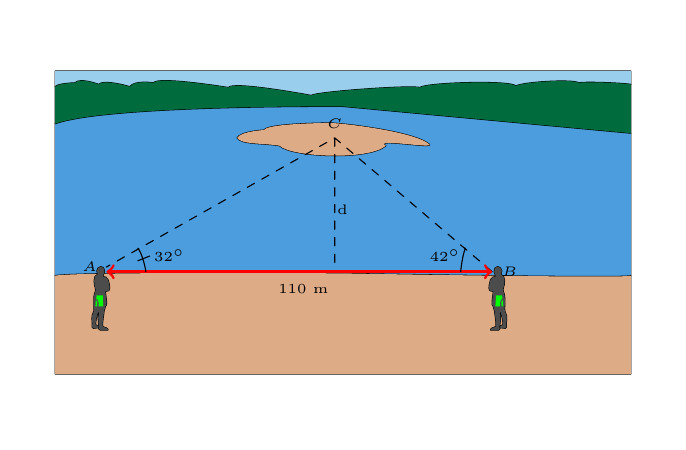
\begin{tikzpicture}[line join=round, line cap=round,scale=1.,transform shape]
			\clip (-4,-2.5) rectangle (4,2.5);
			%\path (0,0) node[opacity=.5,scale=.3] {\includegraphics{h1}};
			%\draw[gray!50] (-4,-2) grid (4,2);
			
			\tikzset{dao/.pic={
					\def\H{ 
						(-1.34,1.1)
						..controls +(60:.1) and +(-160:0) ..  (-1,1.2)
						..controls +(60:.1) and +(140:0) ..  (-.18,1.29)
						..controls +(10:.06) and +(140:0.27) .. (1.1,1.02)
						..controls +(-40:.1) and +(150:0.2) .. (.55,1)
						..controls +(-140:.3) and +(-45:0.2) .. (-.8,1)
						..controls +(170:.2) and +(-60:0.1) .. cycle
						;}
					\draw \H;
					\fill[tumbleweed] \H;
			}}
			\tikzset{nui/.pic={
					\def\T{ %Trời
						(-3.65,1.75)
						..controls +(60:.05) and +(-160:0) ..  (-3.4,1.8)
						..controls +(45:.1) and +(-150:0) ..  (-3.1,1.78)
						..controls +(45:.1) and +(-150:0) ..  (-2.7,1.75)
						..controls +(60:.1) and +(-160:0) ..  (-2.4,1.8)
						..controls +(60:.1) and +(-160:0) ..  (-1.45,1.74)
						..controls +(60:.1) and +(-160:0) ..  (-.4,1.64)
						..controls +(30:.1) and +(160:0.1) ..  (.98,1.74)
						..controls +(40:.1) and +(130:0.1) ..  (2.2,1.76)
						..controls +(30:.1) and +(150:0.1) ..  (3,1.8)
						..controls +(10:.1) and +(170:0.1) ..  (3.66,1.78)--(3.66,1.95)--(-3.65,1.95)--cycle
						;}
					\draw \T;
					\fill[lightcornflowerblue] \T;
					\def\N{ 
						(-3.65,1.75)
						..controls +(60:.05) and +(-160:0) ..  (-3.4,1.8)
						..controls +(45:.1) and +(-150:0) ..  (-3.1,1.78)
						..controls +(45:.1) and +(-150:0) ..  (-2.7,1.75)
						..controls +(60:.1) and +(-160:0) ..  (-2.4,1.8)
						..controls +(60:.1) and +(-160:0) ..  (-1.45,1.74)
						..controls +(60:.1) and +(-160:0) ..  (-.4,1.64)
						..controls +(30:.1) and +(160:0.1) ..  (.98,1.74)
						..controls +(40:.1) and +(130:0.1) ..  (2.2,1.76)
						..controls +(30:.1) and +(150:0.1) ..  (3,1.8)
						..controls +(10:.1) and +(170:0.1) ..  (3.66,1.78)--(3.66,1.16)
						..controls +(175:.2) and +(20:0) ..  (0,1.5)
						..controls +(20:0) and +(20:.7) ..  (-3.65,1.28)--cycle
						;}
					\draw \N;
					\fill[cadmiumgreen] \N;
			}}
			
			\tikzset{bien/.pic={
					\def\B{ 
						(3.66,1.16)
						..controls +(175:.2) and +(20:0) ..  (0,1.5)
						..controls +(20:0) and +(20:.7) ..  (-3.65,1.28)--(-3.65,-.65)
						..controls +(15:.2) and +(120:0) .. (0,-.62)
						..controls +(-60:0) and +(-160:0.1) .. (3.66,-.65)--(3.66,1.16)
						;}
					\draw \B;
					\fill[trueblue!70!] \B;
					\def\C{ %Cát
						(-3.65,-.65)
						..controls +(15:.2) and +(120:0) .. (0,-.62)
						..controls +(-60:0) and +(-160:0.1) .. (3.66,-.65)--(3.66,-1.9)--(-3.65,-1.9)--cycle
						;}
					\draw \C;
					\fill[tumbleweed] \C;
			}}
			
			\tikzset{nguoi/.pic={
					\def\N{ 
						(-3.04,-.64)--(-3.025,-.6)
						..controls +(90:.1) and +(85:0.06) .. (-3.122,-.59)--(-3.11,-.63)
						..controls +(-160:.07) and +(110:0.05) .. (-3.14,-.81)
						..controls +(-40:.01) and +(60:0) .. (-3.14,-.85)
						..controls +(-120:.07) and +(80:0.05) .. (-3.16,-1.1)
						..controls +(-120:.09) and +(80:0.05) .. (-3.18,-1.28)
						..controls +(-120:.02) and +(170:0.01) .. (-3.165,-1.318)--(-3.1,-1.31)--(-3.1,-1.29)
						..controls +(120:.01) and +(-30:0) .. (-3.135,-1.278)
						..controls +(120:.02) and +(-120:0.04) .. (-3.1,-1.1)
						..controls +(-70:.04) and +(120:0.01) ..(-3.096,-1.14)
						..controls +(-120:.04) and +(120:0.01) ..(-3.09,-1.3)
						..controls +(-120:.02) and +(170:0.02) .. (-3.08,-1.34)--(-2.98,-1.34)
						..controls +(70:.03) and +(-70:0.01) .. (-3.045,-1.296)
						..controls +(110:.04) and +(-70:0.01) .. (-3.03,-1.1)
						..controls +(70:.03) and +(-100:0.01) .. (-3.014,-1.04)--(-3,-1.02)
						..controls +(70:.03) and +(-100:0.01) .. (-3.014,-.85)--(-2.97,-.84)
						..controls +(40:.04) and +(-10:0) .. (-2.98,-.7)
						..controls +(110:.04) and +(-20:0.02) .. (-3.043,-.66)--cycle
						;}
					\draw \N;
					\fill[black!70!] \N;
					\def\Q{ %quần
						(-3.045,-.9)
						..controls +(120:.01) and +(-30:0) .. (-3.04,-1.04)
						-- (-3.1,-1.038)
						..controls +(80:.07) and +(-10:0.01) .. (-3.13,-.94)--(-3.124,-.9)--cycle
						(-3.14,-1.04)--(-3.12,-1.04)
						..controls +(80:.07) and +(-10:0.01) .. (-3.134,-.96)--cycle
						;}
					%\draw \Q;
					\fill[green] \Q;
					
			}}
			
			\path
			(0,0)pic[scale=1]{bien} (0,0)pic[scale=1]{dao}
			(0,0)pic[scale=1]{nui}
			(0,0)pic[scale=1]{nguoi} (-1.1,0)pic[scale=1,rotate=180,yscale=-1]{nguoi}
			;
			
			\draw[dashed] (1.9,-.6)node[right]{\tiny $B$}--(-.1,1.1)node[above]{\tiny $C$}--(-3,-.54)node[left]{\tiny $A$} (-.1,1.1)--(-.1,-.6);
			\draw (-2.6,-.46)--(-2.45,-.4);%gạch góc
			\draw[<->,red,line width=1] (-3,-.6)--(1.9,-.6);
			\node at (-.5,-1) [above]{\tiny $110$ m};
			\node at (0,0) [above]{\tiny d};
			\node at (-2.2,-.6) [above]{\tiny $32^\circ$};
			\node at (1.3,-.6) [above]{\tiny $42^\circ$};
			%góc
			\draw (-2.6,-.3)
			..controls +(-50:.09) and +(60:0.01) .. (-2.5,-.6);
			\draw[scale=1,rotate=180,xscale=.6,yscale=-1] (-2.6,-.3)
			..controls +(-50:.09) and +(60:0.01) .. (-2.5,-.6);
		\end{tikzpicture}
		
	\end{center}
	\loigiai{
		\begin{center}
			\begin{tikzpicture}[line join=round, line cap=round,scale=1.5,transform shape]
				\draw (1.9,-.6) node[right]{\tiny $B$}--(-.1,1.1)node[above]{\tiny $C$}--(-3,-.6)node[left]{\tiny $A$}--cycle (-.1,1.1)--(-.1,-.6)node[below]{\tiny $H$};
				\draw (-2.6,-.46)--(-2.45,-.4);%gạch góc
				\node at (-.8,-1) [above]{\tiny $110$ m};
				\node at (0,0) [above]{\tiny d};
				\node at (-2.2,-.6) [above]{\tiny $32^\circ$};
				\node at (1.3,-.6) [above]{\tiny $42^\circ$};
				%góc
				\draw (-2.6,-.37)
				..controls +(-50:.09) and +(60:0.01) .. (-2.5,-.6);
				\draw[scale=1,rotate=180,xscale=.6,yscale=-1] (-2.6,-.3)
				..controls +(-50:.09) and +(60:0.01) .. (-2.5,-.6);
			\end{tikzpicture}
		\end{center}
		Trong tam giác $ ABC $, ta có $ \widehat{ACB}=180^\circ -( \widehat{CAB}+ \widehat{CBA})=180^\circ -(32^\circ+42^\circ)=106^\circ$.\\
		Theo định lý $ \sin $ ta có 
		\[\dfrac{AC}{\sin B}=\dfrac{AB}{\sin C}\Leftrightarrow \dfrac{AC}{\sin 42^\circ}=\dfrac{110}{\sin 106^\circ}\]
		suy ra $AC\approx 76{,}57$.\\
		Diện tích tam giác $ ABC $ là 
		\[S=\dfrac{1}{2}AB\cdot AC\cdot \sin \widehat{CAB}=\dfrac{1}{2}CH\cdot AB\]
		suy ra $ CH=AC\cdot \sin \widehat{CAB} \approx 76{,}57\cdot \sin 32^\circ \approx 40{,}58$.\\
		Vậy khoảng cách từ vị trí $C$ trên đảo tới bờ biển xấp xỉ $ 40{,}58 $ m.
	}
\end{ex}

\begin{ex}%[0H4V3-2]%[Dự án đề cương 3 khối NH24-25 - Đợt 2 - Vũ Ngọc Hào]
	\immini[thm]{Hai trạm quan sát ở hai thành phố Đà Nẵng (giả sử là điểm $B$) và Nha Trang (giả sử là điểm $C$) đồng thời nhìn thấy vệ tinh (giả sử là điểm $A$) với góc nâng lần lượt là $75^\circ$ và $60^\circ$. Tính khoảng cách từ vệ tinh đến trạm quan sát tại thành phố Đà Nẵng và khoảng cách từ vệ tinh đến trạm quan sát tại Nha Trang, biết rằng khoảng cách giữa hai trạm quan sát là $520 \mathrm{~km}$ \textit{(Kết quả làm tròn một chữ số thập phân sau dấu phẩy)}.
	}
	{	
		\begin{tikzpicture}[line join=round, line cap=round,scale=1,transform shape]
			\clip (-1.5,-1.14) rectangle (4.5,3.8);
			\begin{pgfinterruptboundingbox}
				\tikzset{vetinh/.pic={
						\def\D{ 
							(.94,.77)--(1.2,.94)--(.95,.91)--(.85,.85)--cycle
							;}
						\draw \D;
						\fill[gray] \D;
						\def\V{ 
							(.6,.82)--(1.3,.92)--(1.4,1.05)--(.7,.95)--
							cycle;
						}
						\draw \V;
						\fill[pattern=north east lines] \V;
						\def\T{ 
							(.8,.72)--(.84,.9)
							..controls +(40:0.05) and +(120:0.1) .. (1,.75)--cycle;
						}
						\draw \T;
						\fill[black!50!white] \T;
				}}
				%Vẽ nhà 1
				\tikzset{nha/.pic={
						\draw (-1.05,-.25)coordinate [label=above:] (A)--(.12,3.52)coordinate (C)--(3,-.25)coordinate [label=above:] (B)--cycle;
						%\node at (-.68,0) [above]{\tiny $360$ km};
						\node at (.77,-0.7) [above]{\tiny $520$ km};
						%\node at (C) [left]{\tiny $13{,}2^\circ$};
						%\node at ([xshift=0.7cm,yshift=0.3cm]A){\tiny$75^\circ$};
						%\node at ([xshift=-0.7cm,yshift=0.3cm]B){\tiny$60^\circ$};
						%\tkzMarkAngles[size=.5](B,A,C);
						%\tkzMarkAngles[size=.5,double](C,B,A);
						\draw [yellow!40!gray,line width=0.7cm,decorate,decoration={random steps, segment length=1cm}]([yshift=-0.7cm,xshift=-.5]A) -- ([yshift=-0.7cm, xshift=0.3cm]B);
						\node at ([xshift=0.1cm,yshift=-0.75cm]A){\tiny \text{Đà Nẵng}};
						\node at ([yshift=-0.75cm]B){\tiny \text{Nha Trang}};
						\node at ([xshift=0.6cm]C){\tiny \text{Vệ tinh}};
						\def\N{ 
							(-1.22,-.25)--(-.82,-.25)--(-.82,-.85)--(-.82,-.85)--(-1.22,-.85)--cycle;}
						\draw \N;
						\fill[brown] \N;
				}}
				%ve nha 2
				\tikzset{nhahai/.pic={
						\def\NH{ 
							(-1.22,-.25)--(-.82,-.25)--(-.82,-.85)--(-.82,-.85)--(-1.22,-.85)--cycle;}
						\draw \NH;
						\fill[cyan] \NH;
				}}
				\tikzset{cuaso/.pic={
						\def\C{ 
							(-1.22,-.25)--(-.82,-.25)--(-.82,-.85)--(-.82,-.85)--(-1.22,-.85)--cycle;}
						\draw \C;
						\fill[white] \C;
				}}
				\tikzset{cay/.pic={
						\def\C{ 
							(-1.25,-.85)--(-1.24,-.75)--(-1.22,-.75)--(-1.2,-.85)--cycle
							;}
						\def\L{ 
							(-1.23,-.78)
							..controls +(-40:.13) and +(-160:0.16) .. (-1.27,-.7)
							..controls +(-40:.13) and +(-160:0.14) .. (-1.23,-.6)
							..controls +(120:.0) and +(50:0.11) .. (-1.2,-.7)
							..controls +(60:.1) and +(0:0.2) .. (-1.23,-.78)
							--cycle
							;}
						
						\draw \C;
						\fill[black!50!white] \C;
						\draw \L;
						\fill[green] \L;
				}}
				\path(0,0)pic[scale=1]{nha}
				(0,0)pic[fill=white,scale=.2,,xshift=-4.7cm,,yshift=-1.5cm]{cuaso}
				(0,0)pic[fill=white,scale=.2,,xshift=-4.1cm,,yshift=-1.5cm]{cuaso}
				(0,0)pic[fill=white,scale=.2,,xshift=-3.5cm,,yshift=-1.5cm]{cuaso}
				(0,0)pic[fill=white,scale=.4,,xshift=-1.55cm,,yshift=-1.25cm]{cuaso}
				(0,0)pic[scale=1]{cay}
				(4,0)pic[scale=1]{nhahai}
				(3.25,0)pic[fill=white,scale=.4,,xshift=0.35cm,,yshift=-1.25cm]{cuaso}
				(3.25,0)pic[fill=white,scale=.2,,xshift=-1cm,,yshift=-1.5cm]{cuaso}
				(3.25,0)pic[fill=white,scale=.2,,xshift=-.4cm,,yshift=-1.5cm]{cuaso}
				(3.25,0)pic[fill=white,scale=.2,,xshift=.2cm,,yshift=-1.5cm]{cuaso}
				(-0.5,3)pic[scale=.7]{vetinh}
				(3,0.1)pic[scale=1.3]{cay}
				(2,0.2)pic[scale=1.5]{cay}
				;
			\end{pgfinterruptboundingbox}
			\draw pic [draw,"$60^\circ$", angle eccentricity=1.5,angle radius=6 mm] {angle=C--B--A};
			\draw pic [draw,"$75^\circ$",double, angle eccentricity=1.5,angle radius=6 mm] {angle=B--A--C};
		\end{tikzpicture}
	}
	\loigiai{
		\immini{
			Bài toán đưa về tính cạnh $AB, AC$ của tam giác $ABC$ biết $\widehat{B}=75^\circ$, $\widehat{C}=60^\circ$ và $CB=520\text{ km}.$\\
			Ta có $ \widehat{A}=180^\circ-(\widehat{B}+\widehat{C})=45^\circ$\\
			Áp dụng định lí Sin trong tam giác $ABC,$ ta có:
			\begin{itemize}
				\item $\dfrac{AB}{\sin C}=\dfrac{BC}{\sin A}\Rightarrow AB=\dfrac{BC\cdot \sin C}{\sin A}=\dfrac{520\cdot\sin 60^\circ }{\sin 45^\circ}\approx 636{,}9 (\text{km}).$
				\item $\dfrac{AC}{\sin B}=\dfrac{BC}{\sin A}\Rightarrow AC=\dfrac{BC\cdot \sin B}{\sin A}=\dfrac{520\cdot\sin 75^\circ }{\sin 45^\circ}\approx 710{,}3 (\text{km}).$
			\end{itemize}
		}
		{\begin{tikzpicture}[scale=0.5,font=\scriptsize]
				\path
				(0,0) coordinate [label=left:$B$](B)
				(5,0) coordinate [label=right:$C$](C)
				($(B)!2cm!75:(C)$)coordinate[label=left:](m)
				($(C)!2cm!-60:(B)$)coordinate[label=right:](n)
				(intersection of B--m and C--n) coordinate [label=above:$A$](A)
				;
				\foreach \x in{B,C,A}
				{\fill (\x)circle (1.5pt);}
				\draw (A)--(B)--(C)--cycle;
				\path (B)--node [below]{$520\text{ km}$}(C);
				\draw pic ["$75^\circ$",draw, angle eccentricity=1.6,angle radius=0.5cm] 
				{angle=C--B--A};
				\draw pic ["$60^\circ$",double, draw, angle eccentricity=1.6,angle radius=0.5cm] 
				{angle=A--C--B};
		\end{tikzpicture}}
		\noindent Vậy khoảng cách từ vệ tinh đến trạm quan sát tại thành phố Đà Nẵng và trạm quan sát tại Nha Trang lần lượt là $636{,}9 (\text{km})$ và $710{,}3 (\text{km})$.
		
	}
\end{ex}
\begin{ex}%[0H4V3-2]%[Dự án đề cương 3 khối NH24-25 - Đợt 2 - Vũ Ngọc Hào]
	Tại một vị trí $O$ trên bờ biển hai chiếc tàu đi thực hiện khảo sát, chiếc tàu thứ nhất đi vuông góc với bờ biển, chiếc tàu thứ hai đi theo hướng $40^\circ$ so với bờ biển. Sau khi đi được $1$ giờ $30$ phút đến vị trí $A$ thì chiếc tàu thứ nhất bị hỏng và tự sửa chữa trong $30$ phút nhưng không được nên đã gọi cho chiếc tàu thứ hai giúp đỡ. Khi nhận được tin báo thì chiếc tàu thứ hai đang ở vị trí $B$ lập tức đi thẳng đến vị trí chiếc tàu thứ nhất. Hãy tính thời gian mà chiếc tàu thứ hai di chuyển đến hỗ trợ chiếc tàu thứ nhất (tính theo giờ và làm tròn đến chữ số phần trăm) biết rằng toàn bộ quá trình cả hai tàu đều di chuyển với vận tốc không đổi là $40$ km/h.
	\loigiai{
		\immini{
			Ta minh họa bài toán thành hình vẽ như hình bên.
			\begin{itemize}
				\item $OB=40\cdot 2=80$km.
				\item $OA=40\cdot 1{,}5=60$km.
				\item $\widehat{AOB}=90^\circ-40^\circ=50^\circ$.
			\end{itemize}
			Ta có: $\begin{aligned}[t]
				AB=&\, \sqrt{OB^2+OA^2-2\cdot OB\cdot OA\cdot \cos \widehat{AOB}}\\
				=&\, \sqrt{80^2+60^2 -2\cdot 80\cdot 60\cdot \cos 50^\circ}\\
				\Rightarrow AB \approx&\, 61{,}88.
			\end{aligned}$
			
		}{
			\begin{tikzpicture}
				\def\a{3}
				\def\goc{40}
				\def\c{5}
				\path (0,0) coordinate (O)--++(\goc:\c) coordinate (B)
				(O)--++(0,\a) coordinate (A)
				(O)--++(6,0) coordinate (c);
				\draw[line width=1pt, blue] (A)--(O)--(B)--cycle;
				\draw[line width=3pt,dashed, brown] ($(O)+(-1,0)$)--++(6,0)node[below]{\color{black}bờ biển};
				\draw pic[draw,"$40^\circ$" angle radius=3mm,angle eccentricity=2]{angle=c--O--B};
				\foreach \x/\y in {A/90,B/90,O/-90} \fill[black] (\x) circle (1pt) ($(\x)+(\y:5mm)$) node{$\x$};
				\draw (A) node{\faShip};
				\draw (B) node{\faShip};
			\end{tikzpicture}
		}\noindent
		Thời gian chiếc tàu thứ hai di chuyển đến khi gặp tàu thứ nhất: $61{,}88 : 40 \approx 1{,}55$ giờ.
	}
\end{ex}

\begin{ex}[Trích đề kiểm tra Toán khối 10 GHK1 NH24-25-THPT An Lạc]%[0H4V3-2]%[Dự án đề cương 3 khối NH24-25 - Đợt 2 - Vũ Ngọc Hào]
	\immini
	{Hai người đứng trên bờ biển ở hai vị trí $A$, $B$ cách nhau $500$ m cùng nhìn thấy mép của một hòn đảo ở vị trí $C$ trên đảo với các góc so với bờ biển lần lượt là $60^\circ$ và $70^\circ$. Tính khoảng cách $d$ từ mép hòn đảo đến bờ biển (làm tròn đơn vị m).
	}
	{
		\begin{tikzpicture}[line join=round, line cap=round,scale=1.5,transform shape]
			\definecolor{darkbrown}{rgb}{0.4, 0.26, 0.13}	
			\definecolor{lightcornflowerblue}{rgb}{0.6, 0.81, 0.93}
			\definecolor{forestgreen(web)}{rgb}{0.13, 0.55, 0.13}
			\definecolor{darkpastelgreen}{rgb}{0.01, 0.75, 0.24}
			\definecolor{bronze}{rgb}{0.8, 0.5, 0.2}
			\definecolor{deepskyblue}{rgb}{0.0, 0.75, 1.0}
			
			\clip (-1.8,-2.5) rectangle (2.3,1.5);
			\tikzset{gon_song/.pic={
					\def\S{ %sóng
						(-1.35,-2.15)
						..controls +(160:.5) and +(-40:.5) ..(-2.5,-2.15)
						(3.5,-2.2)
						..controls +(160:.2) and +(-40:.5) ..(2,-2.2)
						%----
						(3,-2.5)
						..controls +(160:.5) and +(-40:.5) ..(1.4,-2.5)
						..controls +(160:.5) and +(-40:.5) ..(.3,-2.5)
						..controls +(160:.5) and +(-40:.5) ..(-.75,-2.55)
						;}
					\draw[color=deepskyblue] \S;
			}}
			\tikzset{nuoc/.pic={
					\def\N{ %nước sông
						(-4,.3)
						%..controls +(160:.2) and +(-80:.3)..(1.5,.1)
						..controls +(120:.5) and +(-100:0.2)..(4,.8)--(4,-1.1)
						..controls +(-150:.3) and +(60:.3) ..(2,-1.2)
						..controls +(-100:.5) and +(120:1) ..(-4,-1.9)
						--cycle
						;}
					%\draw \N;
					\fill[lightcornflowerblue] \N;
			}}
			
			\tikzset{dat/.pic={
					\def\T{ %Đất
						(0,0)%trái
						..controls +(170:.2) and +(40:.3) ..  (-.7,-.1)
						..controls +(-120:.15) and +(40:.15) ..  (-1.1,-.25)
						..controls +(-150:.4) and +(170:.4) ..  (-.7,-.55)
						..controls +(-35:.4) and +(-150:.2) ..  (.2,-.7)
						..controls +(50:.4) and +(-120:.35) ..  (.8,-.5)
						..controls +(60:.3) and +(-120:.2) ..  (1.3,-.3)
						..controls +(60:.2) and +(-50:.1) ..  (.7,-.1)
						..controls +(60:.2) and +(-40:.1) ..  (0,0)
						
						;}
					\draw \T;
					\fill[darkbrown] \T;
			}}
			\tikzset{cay/.pic={
					\def\T{ %Thân
						(-.33,0)%trái
						..controls +(-50:.25) and +(40:.45) ..  (-.57,-1.45)
						..controls +(20:.1) and +(-160:.15) ..  (-.1,-1.3)
						..controls +(-120:.1) and +(60:.15) ..  (-.2,-1.6)
						..controls +(-30:.1) and +(-140:.15) ..  (.15,-1.3)
						..controls +(-20:.1) and +(-160:.15) ..  (.57,-1.4)
						..controls +(170:.4) and +(-160:.1) ..  (.35,0)
						..controls +(110:.5) and +(80:.5) ..  (-.33,0)
						;}
					%\draw \T;
					\fill[bronze] \T;
					\def\C{ 
						(0,.3)
						..controls +(-100:.25) and +(-60:.2) ..  (-.3,.1)
						..controls +(-100:.25) and +(-60:.2) ..  (-.6,0)
						..controls +(-120:.45) and +(-110:.35) ..  (-1,.2)
						..controls +(-150:.5) and +(-140:.35) ..  (-1.15,.7)%nút giao
						..controls +(-170:.4) and +(-170:.35) ..  (-1,1.15)
						..controls +(140:.35) and +(110:.4) ..  (-.37,1.35)
						..controls +(110:.25) and +(80:.3) ..  (-.15,1.35)
						..controls +(80:.3) and +(95:.8) ..  (.55,1.1)
						..controls +(80:.2) and +(95:.2) ..  (.8,1.1)
						..controls +(20:.1) and +(95:.1) ..  (.95,1)
						..controls +(-20:.4) and +(35:.25) ..  (1,.47)
						..controls +(-30:.3) and +(-20:.3) ..  (.75,0.05)%nút giao
						..controls +(-120:.3) and +(-60:.2) ..  (.35,0)
						..controls +(175:.2) and +(-160:.1) ..  (.2,0.2)
						..controls +(-160:.1) and +(-70:.1) ..  (0,.3)
						;}
					\draw \C;
					\fill[forestgreen(web)] \C;
					\def\C1{ 
						(-1.15,.7)%nút giao
						..controls +(-170:.4) and +(-170:.35) ..  (-1,1.15)
						..controls +(140:.35) and +(110:.4) ..  (-.37,1.35)
						..controls +(110:.25) and +(80:.3) ..  (-.15,1.35)
						..controls +(80:.3) and +(95:.8) ..  (.55,1.1)
						..controls +(80:.2) and +(95:.2) ..  (.8,1.1)
						..controls +(20:.1) and +(95:.1) ..  (.95,1)
						..controls +(-20:.4) and +(35:.25) ..  (1,.47)
						..controls +(-50:.5) and +(-85:.6) ..  (.65,.55)% gần nút giao
						..controls +(-160:.4) and +(-120:.4) ..  (0,.7)
						..controls +(-150:.2) and +(-80:.4) ..  (-.63,.6)
						..controls +(-140:.5) and +(-130:.4) ..  (-1.15,.7)
						;}
					%\draw \C1;
					\fill[darkpastelgreen] \C1;
					\def\G{ %Gân
						(-.8,.2)
						..controls +(-35:.1) and +(130:.35) ..  
						(-.32,0)%nút giao
						..controls +(-40:.1) and +(45:.35) ..  (-.42,-1.25)
						(-.32,0)%nút giao
						..controls +(120:.1) and +(-45:.35) ..  (-.58,.45)
						(-.32,0)%nút giao
						..controls +(80:.1) and +(-170:.35) ..  (-.05,.45)
						(-.28,.3)
						..controls +(80:.1) and +(-60:.05) ..  (-.35,.55)
						%Gân phải
						(.45,-1.3)
						..controls +(130:.6) and +(-160:.3) ..  (.6,0.35)
						(.37,0)
						..controls +(35:.2) and +(-150:.1) ..  (.66,0.15)
						(.37,0)
						..controls +(80:.2) and +(-40:.1) ..  (.18,0.4)
						(.31,0.25)
						..controls +(80:.1) and +(-150:.1) ..  (.38,0.5)
						(.25,-0.15)
						..controls +(-110:.05) and +(110:.05) ..  (.2,-0.5)%gân dọc
						(.2,-0.25)
						..controls +(-110:.05) and +(110:.05) ..  (.17,-0.45)
						(-.2,-0.15)
						..controls +(-70:.1) and +(110:.05) ..  (-.18,-0.5)
						(-.15,-0.15)
						..controls +(-70:.1) and +(110:.05) ..  (-.15,-0.7)
						(-.05,-0.8)
						..controls +(-80:.15) and +(-10:.15) ..  (-.3,-1.28)
						(-.1,-0.9)
						..controls +(-110:.1) and +(20:.05) ..  (-.2,-1.1)
						(.1,-1)
						..controls +(-50:.05) and +(120:.05) ..  (.15,-1.2)
						(.1,-1.15)
						..controls +(-50:.05) and +(120:.05) ..  (.12,-1.2)
						(.15,-.75)
						..controls +(-120:.1) and +(-140:.1) ..  (.22,-.9)
						..controls +(70:.12) and +(120:.05) ..  (.18,-.9)
						;}
					
					\draw \G;
					
			}}
			\path
			(0,0)pic[scale=1]{nuoc}
			(0,.45)pic[scale=1]{dat}
			%	(0,.5)pic[scale=.6]{cay}
			(0,.5)pic[scale=.6]{gon_song}
			(2,1.5)pic[scale=.6]{gon_song}
			(-2.5,1.3)pic[scale=.5]{gon_song}
			;
			\path 	(2,-1.5) coordinate (A)
			(-1,-1.5) coordinate (B)
			(0,-.3) coordinate (C)
			;
			\node at (B) [left]{\tiny $B$};
			\node at (A) [right]{\tiny $A$};
			\node[white] at (C) [above]{\tiny $C$};
			\node at (0.5,-1.4) [below]{\tiny $500$ m};
			\draw (B)--(C)--(A)--cycle;
			\draw    pic["\tiny $60^\circ$", draw=black, angle eccentricity=1.6,angle radius=.4cm, color=blue]
			{angle=C--A--B};
			\draw    pic["\tiny $70^\circ$", draw=black, angle eccentricity=1.6, angle radius=.4cm, color=blue]
			{angle=A--B--C};
			\draw pic[draw, double, cap=butt, angle radius=12pt]{angle=A--B--C};
		\end{tikzpicture}
	}
	\loigiai{
		\immini
		{
			Gọi $CH$ là đường cao của $\triangle ABC$.\\
			Ta có $\widehat{C}=180^\circ-\widehat{A}-\widehat{B}=180^\circ-60^\circ-70^\circ=50^\circ$.\\
			Áp dụng định lý sin vào $\triangle ABC$ có
			$$\dfrac{AC}{\sin B}=\dfrac{AB}{\sin C}\Rightarrow AC=\dfrac{AB\cdot \sin B}{\sin C}=\dfrac{500\cdot \sin 70^\circ}{\sin 50^\circ}\approx 613.$$
		}
		{
			\begin{tikzpicture}[line join=round, line cap=round,scale=1.5,transform shape]
				\path 	(2,-1.5) coordinate (A)
				(-1,-1.5) coordinate (B)
				(0,-.3) coordinate (C)
				($(A)!(C)!(B)$)coordinate(H)
				;
				\node at (B) [left]{\tiny $B$};
				\node at (A) [right]{\tiny $A$};
				\node at (C) [above]{\tiny $C$};
				%	\node at (0.5,-1.4) [below]{\tiny $500$ m};
				\node at (H) [below]{\tiny $H$};
				\draw (B)--(C)--(A)--cycle (C)--(H);
				\draw  pic["\tiny $60^\circ$", draw=black, angle eccentricity=1.6,angle radius=.4cm, color=blue]
				{angle=C--A--B};
				\draw pic["\tiny $70^\circ$", draw=black, angle eccentricity=1.6, angle radius=.4cm, color=blue]
				{angle=A--B--C};
				\draw pic[draw, double, cap=butt, angle radius=12pt]{angle=A--B--C};
				\pic[draw,thin,angle radius=2mm] {right angle=B--H--C};
			\end{tikzpicture}
		}
		\noindent
		Ta lại có $\sin A=\dfrac{CH}{AC}\Rightarrow CH=AC\cdot\sin A=613\cdot\sin 60^\circ\approx 531$ (m).\\
		Vậy khoảng cách $d$ gần bằng $531$ m.
	}
\end{ex}

\begin{ex}[Trích đề kiểm tra Toán khối 10 GHK1 NH24-25- THPT Nguyễn Du-TP HCM]%[0H4V3-2]%[Dự án đề cương 3 khối NH24-25 - Đợt 2 - Vũ Ngọc Hào]
	\immini{
		Hai máy bay cùng cất cánh từ một sân bay nhưng bay theo hai hướng khác nhau. Một chiếc di chuyển với tốc độ $500$ km/h theo hướng tây và chiếc còn lại di chuyển theo hướng lệch so với hướng bắc $35^\circ$ về phía tây với tốc độ $650$ km/h. Sau $90$ phút, hai máy bay cách nhau bao nhiêu kilômét? Giả sử chúng đang ở cùng độ cao.	%Điền câu hỏi
	}
	{
		\begin{tikzpicture}[scale=0.7, font=\footnotesize, line join=round, line cap=round, >=stealth]
			\path
			(0,0) coordinate (A)
			(6,0) coordinate (O)
			(3,5) coordinate (B)
			;
			\draw (A) -- (O) -- (B);
			\draw [dashed] (A) -- (B);
			\fill[black](O) circle (1.5pt);
			\draw (B) node [above]{B}
			(O) node [right]{O}
			(A) node [below]{A};
			\draw (A) -- (O) node [sloped,midway,below]{$500$ km/h}; 	
			\draw (B) -- (O) node [sloped,midway,below]{$650$ km/h};
			\draw [->] (O)--(A);
			\draw [->] (O)--(B);
			\draw [->] (O)--(6,5);
			\draw (-0.5,0) node{Tây} (6,5) node[above]{Bắc};
			\draw (5.6,1.5) node{$35^\circ$};
		\end{tikzpicture}	%Chèn hình
	}
	\loigiai{
		Sau $90$ phút:
		\begin{itemize}
			\item Máy bay đầu tiên bay được $\dfrac{500\cdot 90}{60}= 750$ km.
			\item Máy bay thứ hai bay được $\dfrac{650\cdot 90}{60}= 975$ km.
		\end{itemize}
		Hai máy bay di chuyển lệch nhau một góc $90^\circ-35^\circ=55^\circ$.\\
		Ta có tam giác $ABO$ với $OA=750$ km, $OB=975$ km và $\widehat{BOA}=55^\circ$.\\
		Áp dụng định lí côsin, ta có
		\[AB^2=OA^2+OB^2-2\cdot OA \cdot OB \cdot \cos \widehat{BOA}=750^2+975^2-2\cdot 750 \cdot 975 \cdot \cos 55^\circ \approx 674\;269{,}46.\]
		Suy ra $AB=\sqrt{674\;269{,}46}\approx 821{,}14$ km.\\
		Vậy sau $90$ phút hai máy bay cách nhau	$821{,}14$ km.
	}
\end{ex}

\begin{ex}%[0H1V3-2]%[Dự án đề cương 3 khối NH24-25 - Đợt 2 - Vũ Ngọc Hào]
	\immini[thm]{
		Từ hai vị trí $A$ và $B$ của một tòa nhà, người ta quan sát đỉnh $C$ của ngọn núi. Biết rằng độ cao $AB=70$ m, phương nhìn $AC$ tạo với phương nằm ngang một góc $30^\circ$. Phương nhìn $BC$ tạo với phương nằm ngang một góc $15^\circ30'$. Khi đó chiều cao của ngọn núi so với mặt đất là bao nhiêu? (\textit{làm tròn đến hàng đơn vị})
	}{
		\begin{tikzpicture}[x=2.5mm,y=2.5mm,blue,thick, font=\footnotesize, line cap=round, line join=round]
			\def\a{1}
			\path 	
			(0:0) coordinate (A)
			($(A)+(0:1)$) coordinate (A1)
			($(A)+(30:1)$) coordinate (A2)
			(90:7*\a) coordinate (B)
			($(B)+(0:1)$) coordinate (B1)
			($(B)+(31/2:1)$) coordinate (B2)
			(180:3*\a) coordinate (A')
			($(B)+(A')-(A)$) coordinate (B')
			(intersection of A--A2 and B--B2) coordinate (C)
			(intersection of A--A2 and B--B1) coordinate (I)
			($(A)!(C)!(A1)$) coordinate (H)
			($(B)!(C)!(B1)$) coordinate (K)
			($(H)!1/3!(A)$) coordinate (Ht)
			($(H)!-1/3!(A)$) coordinate (Hp)
			($(C)!2/3!(Ht)$) coordinate (m)
			($(C)!2/3!(Hp)$) coordinate (n)
			($(C)!1/4!(Ht)$) coordinate (p)
			($(C)!1/4!(Hp)$) coordinate (q)
			($(C)+(Hp)-(H)$) coordinate (Cp)
			;
			\draw (A)--(B) node[pos=.575,right]{70 m}--(B')--(A')--cycle (C)--(H)--(A)--(C)--(B)--(K) ;
			\draw[teal,thin] 
			($(A)!1/4!(B)$)--($(A')!1/4!(B')$)
			($(A)!2/4!(B)$)--($(A')!2/4!(B')$)
			($(A)!3/4!(B)$)--($(A')!3/4!(B')$)
			($(A)!1/2!(A')$)--($(B)!1/2!(B')$)
			;
			\pic[draw,angle radius=6mm,angle eccentricity=1.75,"$30^\circ$"] {angle=H--A--C};
			\pic[draw,angle radius=12mm,angle eccentricity=1.65,"$15^\circ30'$"] {angle=K--B--C};
			\foreach \x/\g in {A/-90,B/90,C/90,I/-90}
			\fill[black] (\x) circle (1pt) ($(\g:3mm)+(\x)$) node {$\x$};
			
			\draw[clip]
			decorate [decoration={random steps,segment length=9pt,amplitude=3pt}]%
			{(Ht) -- ($(m)+(180:2mm)$) -- (C) -- ($(n)+(0:3mm)$) -- (Hp)}
			-- ($(Hp)+(-90:3mm)$) -- ($(Ht)+(-90:3mm)$) -- (Ht) ;
			\fill[brown,opacity=.85]($(Ht)+(-90:3mm)$) rectangle (Cp);
			\fill[green,opacity=.85]($(Ht)+(-90:3mm)$) rectangle (Hp);
			\fill[white,opacity=.85]
			decorate [decoration={random steps,segment length=3pt,amplitude=1pt}]%
			{(C) -- ($(p)+(0:.09mm)$) -- ($(p)+(-80:13mm)$) -- ($(p)+(-10:3mm)$) -- ($(p)+(-50:10mm)$) -- ($(p)+(15:6mm)$) -- ($(q)+(180:.25pt)$)} -- cycle ;
			\path (K) node[above right]{$K$} (H) node[above right]{$H$};
			\fill[black]  (K) circle(1pt) (H) circle(1pt) (C) circle(1pt) ;
			\draw (C)--(H);
		\end{tikzpicture}
	}
	\loigiai{
		Ta có 
		$\begin{aligned}[t]
			& \widehat{ABC}=\widehat{ABK}+\widehat{KBC}=90^{\circ}+15^{\circ}30'=105^{\circ}30'.\\
			& \widehat{BAC}=\widehat{BAH}-\widehat{CAH}=90^{\circ}-30^{\circ}=60^{\circ}.\\
			\Rightarrow & \widehat{ACB}=180^{\circ}-\widehat{BAC}-\widehat{ABC}=14^{\circ}30'.
		\end{aligned}$\\
		Áp dụng định lí $\sin$ cho $\triangle ABC$, ta có \\
		$\dfrac{AB}{\sin\widehat{ACB}}=\dfrac{AC}{\sin\widehat{ABC}}$  
		$\Rightarrow AC=\dfrac{AB\cdot\sin\widehat{ABC}}{\sin\widehat{ACB}}= \dfrac{70\cdot\sin105^{\circ}30'}{\sin14^{\circ}30'}\approx269$ (m).\\
		Xét $\triangle ACH$ vuông tại $H$, ta có $CH=AC\cdot\sin\widehat{CAH}=\dfrac{70\cdot\sin105^{\circ}30'}{\sin14^{\circ}30'}\cdot\sin30^{\circ}\approx 135$ (m).\\
	}
\end{ex}
\begin{ex}%[0H4V3-2]%[Dự án đề cương 3 khối NH24-25 - Đợt 2 - Vũ Ngọc Hào]
	\immini
	{Hai chiếc tàu thuỷ $P$ và $Q$ cách nhau $300$ m và thẳng hàng với chân $B$ của tháp hải đăng $AB$ ở trên bờ biển. Từ $P$ và $Q$, người ta nhìn thấy tháp hải đăng $AB$ dưới các góc $\widehat{BPA}=35^{\circ}$ và $\widehat{BQA}=48^{\circ}$. Tính chiều cao của tháp hải đăng đó.
	}
	{
		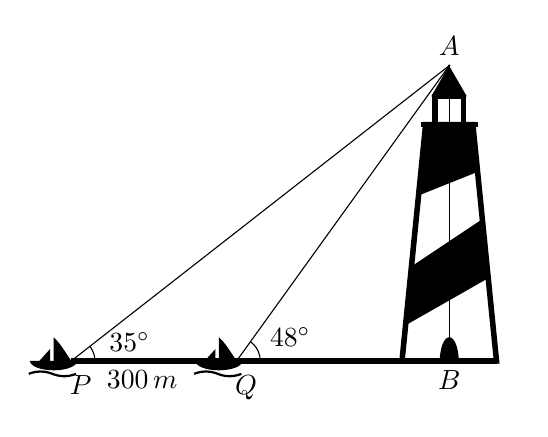
\begin{tikzpicture}[scale=.3]
			\draw [line width=2pt] (0,0)--(1,10)--(3,10)--(4,0)--cycle;
			\fill (3,10)--(3.2,8)--(0.7,7)--(1,10)--cycle;
			\fill (0.14,1.5)--(0.4,4)--(3.4,6)--(3.65,3.5)--cycle;
			\fill (2.4,0) arc(0:180:0.4 cm and 1 cm);
			\draw[line width=2pt] (4,0)--(-14,0);
			\draw[line width=2pt] (0.8,10)--(3.2,10);
			\draw[line width=2pt] (1.4,10)--++(90:1.2)--++(0:1.2)--++(-90:1.2);
			\fill (1.24,11.2)--++(0:1.5)--++(120:1.5)--cycle;
			\begin{scope}
				\draw (-14,0)--(2,12.5);
				\clip (2,12.5) -- (-14,0) -- (5,0);
				\draw (-14,0) circle (1cm);
				\draw (-13+0.2,0) node[above right]{$35^\circ$};
			\end{scope}
			\begin{scope}
				\draw (-7,0)--(2,12.5);
				\clip (2,12.5) -- (-7,0) -- (5,0);
				\draw (-7,0) circle (1cm);
				\draw (-6,0.2) node[above right]{$48^\circ$};
			\end{scope}
			\draw (2,0)--(2,12.5);
			\draw (-11,0) node[below]{$300\,m$};
			\fill (2,12.5) circle (1.5pt) node[above]{$A$};
			\fill (2,0) circle (1.5pt) node[below]{$B$};
			\draw (-14+0.4,0-0.2) node[below]{$P$};
			\draw (-7+0.4,0-0.2)  node[below]{$Q$};
			\fill (-13.75,0) arc(0:-180:1 cm and 0.4 cm);
			\fill (-14,0)..controls(-14.5,0.75)..(-14.75,1)--(-14.75,0);
			\fill (-15.35,0)--(-15+0.1,0.5)--(-15+0.1,0)--cycle;
			\draw[thick] (-15.5-0.3,-0.75+0.2) parabola bend (-15.5+0.5-0.3,-0.75+0.1+0.2) (-15+0.5-0.3,-0.75+0.2) parabola bend (-14.5+0.5-0.3,-0.75-0.1+0.2) (-14+0.5-0.3,-0.75+0.2);
			\fill (-6.75,0) arc(0:-180:1 cm and 0.4 cm);
			\fill (-7,0)..controls(-7.5,0.75)..(-7.75,1)--(-7.75,0);
			\fill (-8.35,0)--(-8+0.1,0.5)--(-8+0.1,0)--cycle;	
			\draw[thick] (-8.5-0.3,-0.75+0.2) parabola bend (-8.5+0.5-0.3,-0.75+0.1+0.2) (-8+0.5-0.3,-0.75+0.2) parabola bend (-7.5+0.5-0.3,-0.75-0.1+0.2) (-7+0.5-0.3,-0.75+0.2);
			%%hình được vẽ bởi %%sang nguyễn văn
		\end{tikzpicture}
	}
	\loigiai{
		\immini
		{
			Trong tam giác $\triangle APQ$, ta có $\widehat{PQA}=180^\circ-48^\circ=132^\circ$ và $\widehat{PAQ}=180^\circ-132^\circ-35^\circ=13^\circ$.\\
			Áp dụng định lý sin trong tam giác $\triangle APQ$, ta được $$\dfrac{AP}{\sin\widehat{PQA}}=\dfrac{PQ}{\sin\widehat{PAQ}}\Leftrightarrow AP=\dfrac{PQ\cdot\sin\widehat{PQA}}{\sin\widehat{PAQ}} \Leftrightarrow AP=\dfrac{300\cdot \sin{132^\circ}}{\sin{13^\circ}}.$$
			Trong tam giác $\triangle ABP$, ta có
			$$AB=AP\cdot\sin\widehat{APQ}=\dfrac{300\cdot \sin{132^\circ}}{\sin{13^\circ}}\cdot\sin{35^\circ}\approx 568{,}46\,\text{m.}$$
			Vậy chiều cao của tháp hải đăng là $h\approx 568{,}46$ m.
		}
		{
			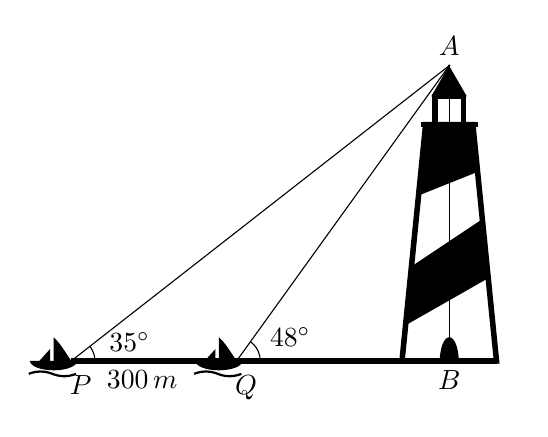
\begin{tikzpicture}[scale=.3]
				\draw [line width=2pt] (0,0)--(1,10)--(3,10)--(4,0)--cycle;
				\fill (3,10)--(3.2,8)--(0.7,7)--(1,10)--cycle;
				\fill (0.14,1.5)--(0.4,4)--(3.4,6)--(3.65,3.5)--cycle;
				\fill (2.4,0) arc(0:180:0.4 cm and 1 cm);
				\draw[line width=2pt] (4,0)--(-14,0);
				\draw[line width=2pt] (0.8,10)--(3.2,10);
				\draw[line width=2pt] (1.4,10)--++(90:1.2)--++(0:1.2)--++(-90:1.2);
				\fill (1.24,11.2)--++(0:1.5)--++(120:1.5)--cycle;
				\begin{scope}
					\draw (-14,0)--(2,12.5);
					\clip (2,12.5) -- (-14,0) -- (5,0);
					\draw (-14,0) circle (1cm);
					\draw (-13+0.2,0) node[above right]{$35^\circ$};
				\end{scope}
				\begin{scope}
					\draw (-7,0)--(2,12.5);
					\clip (2,12.5) -- (-7,0) -- (5,0);
					\draw (-7,0) circle (1cm);
					\draw (-6,0.2) node[above right]{$48^\circ$};
				\end{scope}
				\draw (2,0)--(2,12.5);
				\draw (-11,0) node[below]{$300\,m$};
				\fill (2,12.5) circle (1.5pt) node[above]{$A$};
				\fill (2,0) circle (1.5pt) node[below]{$B$};
				\draw (-14+0.4,0-0.2) node[below]{$P$};
				\draw (-7+0.4,0-0.2)  node[below]{$Q$};
				\fill (-13.75,0) arc(0:-180:1 cm and 0.4 cm);
				\fill (-14,0)..controls(-14.5,0.75)..(-14.75,1)--(-14.75,0);
				\fill (-15.35,0)--(-15+0.1,0.5)--(-15+0.1,0)--cycle;
				\draw[thick] (-15.5-0.3,-0.75+0.2) parabola bend (-15.5+0.5-0.3,-0.75+0.1+0.2) (-15+0.5-0.3,-0.75+0.2) parabola bend (-14.5+0.5-0.3,-0.75-0.1+0.2) (-14+0.5-0.3,-0.75+0.2);
				\fill (-6.75,0) arc(0:-180:1 cm and 0.4 cm);
				\fill (-7,0)..controls(-7.5,0.75)..(-7.75,1)--(-7.75,0);
				\fill (-8.35,0)--(-8+0.1,0.5)--(-8+0.1,0)--cycle;	
				\draw[thick] (-8.5-0.3,-0.75+0.2) parabola bend (-8.5+0.5-0.3,-0.75+0.1+0.2) (-8+0.5-0.3,-0.75+0.2) parabola bend (-7.5+0.5-0.3,-0.75-0.1+0.2) (-7+0.5-0.3,-0.75+0.2);
				%%hình được vẽ bởi %%sang nguyễn văn
			\end{tikzpicture}
		}
		
	}
\end{ex}

\begin{ex}%[0H4V3-2]%[Dự án đề cương 3 khối NH24-25 - Đợt 2 - Vũ Ngọc Hào]
	\immini{Một cây cổ thụ mọc thẳng đứng bên lề một con dốc có độ dốc $8^{\circ}$ so với phương nằm ngang. Từ một điểm dưới chân dốc, cách gốc cây $28$ m người ta nhìn thấy đỉnh ngọn cây dưới một góc $40^{\circ}$ so với phương ngang. Tính chiều cao của cây đó	(làm tròn đến hàng đơn vị, theo đơn vị mét).}
	{
		\usetikzlibrary{decorations.pathmorphing,shapes}
		\tikzset{
			treetop/.style={
				decoration={random steps, segment length=0.4mm},
				decorate
			},
			trunk/.style={
				decoration={random steps, segment length=2mm, amplitude=0.2mm},
				decorate
			}
		}
		\tikzset{
			man/.pic={%
				\fill [rounded corners=1.5] (0,0.4) -- (0,0.4 -- (0.4,0.5 -- (0.4,0.4) --
				(0.325,0.4) -- (0.325,0.7) -- (0.3,0.7) -- (0.3,0) -- (0.225,0) --
				(0.225,0.4) -- (0.175,0.4) -- (0.175,0) -- (0.1,0) -- (0.1,0.7) --
				(0.075,0.7) -- (0.075,0.4) -- cycle;
				\fill (0.2,0.9) circle (0.1);
				\coordinate (-head) at (0.2,1);
				\coordinate (-foot) at (0.2,0);
			}
		}
		\begin{tikzpicture}
			\path 
			(0,1.5) coordinate (C)
			(-5,-5) coordinate (H)
			(0,-3) coordinate (B)
			(0,-5) coordinate (B1)		
			;
			%\pic[red] at (-6.3,-3) (myman) {man};
			\foreach \w/\f in {0.3/30,0.2/50,0.1/70} {
				\fill [brown!\f!black, trunk] (0,0) ++(-\w/2,0) rectangle +(\w,-3);
			}
			\foreach \n/\f in {1.4/40,1.2/50,1/60,0.8/70,0.6/80,0.4/90} {
				\fill [green!\f!black, treetop] ellipse (\n/1.5 and \n);
			}
			\draw (B)--(B1)--(H)--(C)  (B)--(H);
			\pic[draw,"$8^{\circ}$", angle eccentricity=1.3,angle radius=0.8cm]{angle=B1--H--B};
			\pic[draw,"$40^{\circ} $", angle eccentricity=1.6,angle radius=0.7cm]{angle=B1--H--C};
			\draw pic[draw, angle radius=2mm]{right angle=B--B1--H};
			\path (H)--(B) node[below,midway,sloped]{$28$ m};
			%	\foreach \x/\g in {} \fill[black] (\x)+(\g:.3) node {$\x$};
		\end{tikzpicture}
	}
	\loigiai{
		\immini{
			Đặt tên các điểm $B$, $H$, $C$, $A$ như hình vẽ.\\
			Khi đó $BC$ là chiều cao của cây.\\
			Theo đề ta có $\widehat{BHA}=8^{\circ}$, $\widehat{CHA}=40^{\circ}$, từ đó ta có $\widehat{CHB}=32^{\circ}$. \\
			Bên cạnh đó ta có tam giác $BHA$ vuông tại $A$ nên $\widehat{ABH}=82^{\circ}$.\\
			Mà $\widehat{CBH}+\widehat{ABH}=180^{\circ}$ nên $\widehat{CBH}=98^{\circ}$.\\
			Ta có $\widehat{CHB}+ \widehat{CBH}+\widehat{BHC}=180^{\circ} \Rightarrow \widehat{BHC}=50^{\circ}$.
			Áp dụng định lý $\sin$ vào tam giác $BCH$ ta có
			\begin{eqnarray*}
				&&\dfrac{BC}{\sin \widehat{CHB}}=\dfrac{HB}{\sin \widehat{BCH}} \\
				&\Rightarrow& BC=\dfrac{HB \sin \widehat{CHB}}{\sin \widehat{BCH}}=\dfrac{28 \cdot \sin 32^{\circ}}{\sin 50^{\circ}}\approx 19 \ (\mathrm{m}).
			\end{eqnarray*}
			
		}{
			\usetikzlibrary{decorations.pathmorphing,shapes}
			\tikzset{
				treetop/.style={
					decoration={random steps, segment length=0.4mm},
					decorate
				},
				trunk/.style={
					decoration={random steps, segment length=2mm, amplitude=0.2mm},
					decorate
				}
			}
			\tikzset{
				man/.pic={%
					\fill [rounded corners=1.5] (0,0.4) -- (0,0.4 -- (0.4,0.5 -- (0.4,0.4) --
					(0.325,0.4) -- (0.325,0.7) -- (0.3,0.7) -- (0.3,0) -- (0.225,0) --
					(0.225,0.4) -- (0.175,0.4) -- (0.175,0) -- (0.1,0) -- (0.1,0.7) --
					(0.075,0.7) -- (0.075,0.4) -- cycle;
					\fill (0.2,0.9) circle (0.1);
					\coordinate (-head) at (0.2,1);
					\coordinate (-foot) at (0.2,0);
				}
			}
			\begin{tikzpicture}
				\path 
				(0,1.5) coordinate (C)
				(-5,-5) coordinate (H)
				(0,-3) coordinate (B)
				(0,-5) coordinate (A)		
				;
				%\pic[red] at (-6.3,-3) (myman) {man};
				\foreach \w/\f in {0.3/30,0.2/50,0.1/70} {
					\fill [brown!\f!black, trunk] (0,0) ++(-\w/2,0) rectangle +(\w,-3);
				}
				\foreach \n/\f in {1.4/40,1.2/50,1/60,0.8/70,0.6/80,0.4/90} {
					\fill [green!\f!black, treetop] ellipse (\n/1.5 and \n);
				}
				\draw (B)--(A)--(H)--(C)  (B)--(H);
				\pic[draw,"$8^{\circ}$", angle eccentricity=1.4,angle radius=0.8cm]{angle=A--H--B};
				\pic[draw,"$40^{\circ} $", angle eccentricity=1.6,angle radius=0.7cm]{angle=A--H--C};
				\draw pic[draw, angle radius=2mm]{right angle=B--A--H};
				\path (H)--(B) node[below,midway,sloped]{$28$ m};
				\foreach \t/\g in {A/-90,C/90,B/0,H/180}{\draw[fill=white] (\t) circle (1pt) node[shift={(\g:8pt)},font=\footnotesize]{$ \t $};}
			\end{tikzpicture}
		}
	}
\end{ex}
\begin{ex}%[0H4V3-2]%[Dự án đề cương 3 khối NH24-25 - Đợt 2 - Vũ Ngọc Hào]
	Có hai bạn An và Bình đang ở một tòa nhà. Từ chân của một tòa nhà, An phải nhìn góc $22^{\circ}$ trở lên để nhìn ngọn cây. Từ trên cùng của tòa nhà cao $150\mathrm{\,m}$ so với mặt đất, Bình phải nhìn xuống một góc $50^{\circ}$ dưới phương ngang để ngắm ngọn cây. Tính chiều cao của cây?	
	\begin{center}
		\definecolor{lightcornflowerblue}{rgb}{0.6, 0.81, 0.93}
		\definecolor{cadmiumgreen}{rgb}{0.0, 0.42, 0.24}
		\definecolor{trueblue}{rgb}{0.0, 0.45, 0.81}
		\definecolor{tumbleweed}{rgb}{0.87, 0.67, 0.53}%màu cát
		\definecolor{burntumber}{rgb}{0.54, 0.2, 0.14}
		
		\begin{tikzpicture}[line join=round, line cap=round,scale=1.5,transform shape]
			\clip (-4,-3.3) rectangle (3,1.1);
			
			\tikzset{toa_nha_2/.pic={
					\draw[fill=trueblue] (-3,-2.4) rectangle (-.9,1.8);
					\draw[fill=white] (-3,-.19) rectangle (-.9,-.12);
					\draw[fill=white] (-3,-2.39) rectangle (-.9,-2.32);
					\draw[fill=trueblue] (-3.05,1.45) rectangle (-.85,1.8);
			}}
			
			\tikzset{cua/.pic={
					\draw[fill=white] (-1.05,.9) rectangle (-1.35,1.4);
					\draw[fill=white] (-1.55,.9) rectangle (-1.85,1.4);
					\draw[fill=white] (-2.05,.9) rectangle (-2.35,1.4);
					\draw[fill=white] (-2.55,.9) rectangle (-2.85,1.4);
			}}
			
			%%%%%%%%%%%%%%%%%%%%%%%%%%%%%%%%%
			\tikzset{cay/.pic={%Cây
					\def\T{ 
						(-1.73,-2.85)
						..controls +(40:.03) and +(40:.01) ..  (-1.74,-2.7)
						..controls +(140:.04) and +(60:.02) ..  (-1.78,-2.6)
						..controls +(140:.04) and +(60:.02) ..  (-1.8,-2.55)
						..controls +(100:.03) and +(70:.02) ..  (-1.82,-2.5)
						..controls +(140:.04) and +(60:.02) ..  (-1.815,-2.4)
						..controls +(140:.04) and +(60:.02) ..  (-1.818,-2.3)
						..controls +(85:.03) and +(-30:.03) ..  (-1.8,-2.2)
						..controls +(80:.04) and +(50:.02) ..  (-1.78,-2)
						..controls +(60:.04) and +(120:.02) ..  (-1.76,-1.9)
						..controls +(80:.03) and +(-100:.02) ..  (-1.74,-1.8)
						..controls +(80:.01) and +(-100:.02) ..  (-1.72,-1.9)
						..controls +(60:.02) and +(-120:.02) ..  (-1.7,-2)
						..controls +(-80:.02) and +(110:.03) ..  (-1.66,-2.2)
						..controls +(-100:.02) and +(60:.03) ..  (-1.64,-2.3)
						..controls +(-30:.02) and +(70:.02) ..  (-1.6,-2.44)
						..controls +(-100:.02) and +(70:.02) ..  (-1.63,-2.52)
						..controls +(-60:.02) and +(70:.01) ..  (-1.66,-2.6)
						..controls +(60:.01) and +(70:.02) ..  (-1.7,-2.7)
						..controls +(-120:.02) and +(120:.03) ..  (-1.68,-2.85)
						;}
					\draw \T;
					\fill[cadmiumgreen!90!] \T;
			}}
			%%%%%%%%%%%%%%%%%%%%%%
			
			\path 
			(-1,-1)pic[scale=.82,yscale=1]{toa_nha_2}
			(-1.1,-1.3)pic[scale=.78]{cua}
			(-1.1,-1.73)pic[scale=.78]{cua}
			(-1.1,-2.4)pic[scale=.78]{cua}
			(-1.1,-2.9)pic[scale=.78]{cua} 
			(5.5,1.33)pic[xscale=2.5,yscale=1.5]{cay}
			;
			\draw[fill=white] (-2.6,-2.8) rectangle (-2,-2.3);
			\draw[fill=white] (-3.2,-2.8) rectangle (-2.6,-2.3);
			
			\path (-1.72,.47) coordinate (B)
			(2.95,0) coordinate (B2)
			(-1.72,-2.95) coordinate (C)
			(1.15,-1.35) coordinate (A)
			(C)--++(3,0) coordinate(H)
			;
			\draw (B)--(A)--(C)--(3,-2.95);
			\node at (A) [above]{\tiny $A$};
			\node at (B) [above left]{\tiny $B$};
			\node at (C) [below]{\tiny $C$};
			
			\node at (-.9,-1.2) [left]{\tiny $150$ m};
			\draw    pic["\tiny $50^\circ$", double,draw=black, angle eccentricity=1.5, angle radius=.4cm, color=blue]
			{angle=C--B--A}; 
			\draw    pic["\tiny $22^\circ$",draw=black, angle eccentricity=1.5, angle radius=.6cm, color=blue]
			{angle=H--C--A}; 
			%			\draw    pic["\tiny $68^\circ$",draw=black, angle eccentricity=1.5, angle radius=.4cm, color=blue]
			%			{angle=A--C--B}; 	
			
			
		\end{tikzpicture}
	\end{center}
	\loigiai{
		\begin{center}
			\begin{tikzpicture}[line join=round, line cap=round,>=stealth,thick]
				\tikzset{every node/.style={scale=0.9}}
				\draw (0,0)coordinate(C) --++(3,0)coordinate(H) --++(0,2)coordinate(A)--++(-3,3)coordinate(B) --cycle node[pos=0.5,right]{$150$ m}
				(A)--(C);
				\draw pic[draw, "$50^{\circ}$", angle eccentricity=1.5,angle radius=0.6cm] {angle=C--B--A}; 
				\draw pic[draw, "$22^{\circ}$", angle eccentricity=1.5,angle radius=0.8cm] {angle=H--C--A};
				\draw pic[draw, "$68^{\circ}$", angle eccentricity=1.5,angle radius=1cm] {angle=A--C--B};
				\draw pic[draw,  angle eccentricity=1.5,angle radius=0.4cm] {right angle=C--H--A};
				\foreach \p/\q in {A/90,B/90,C/-90,H/-90}{
					\path (\p) node[shift={(\q:3mm)}]{$\p$};
					\fill[black] (\p) circle (1pt);} 
			\end{tikzpicture}
		\end{center}
		Chiều cao của cây là $AH$.\\
		Xét tam giác $ABC$ ta có $\widehat{BAC}=180^{\circ}-50^{\circ}-68^{\circ}=62^{\circ}.$\\
		Áp dụng định lí sin ta có
		$$\dfrac{AC}{\sin 50^{\circ}}=\dfrac{BC}{\sin 62^{\circ}}\Rightarrow AC=\dfrac{BC\cdot \sin 50^{\circ} }{\sin 62^{\circ}}=\dfrac{150\cdot \sin 50^{\circ} }{\sin 62^{\circ}}.$$
		Suy ra chiều cao cây là
		$$AH= AC\cdot \sin 22^{\circ}=\dfrac{150\cdot \sin 50^{\circ} }{\sin 62^{\circ}}\cdot \sin 22^{\circ}\approx 49 \text{ (m)}.$$
	}
\end{ex}

\begin{ex}%[0H4V3-2]%[Dự án đề cương 3 khối NH24-25 - Đợt 2 - Vũ Ngọc Hào]
	Một người đứng tại vị trí $M$ trên tàu neo đậu giữa biển nhìn thấy trên bờ biển có hai ngọn hải đăng ở hai vị trí $A$ và $B$ cách nhau $5$ km. Người đó xác định các góc tạo thành giữa các đường ngắm hai ngọn hải đăng $MA$, $MB$ và đường thẳng $MH$ vuông góc với đường thẳng $AB$ nối hai ngọn hải đăng lần lượt là $35^\circ$ và $15^\circ$ như hình vẽ sau
	\begin{center}
		\definecolor{lightcornflowerblue}{rgb}{0.6, 0.81, 0.93}
		\definecolor{deepskyblue}{rgb}{0.0, 0.75, 1.0}
		\definecolor{cerulean}{rgb}{0.0, 0.48, 0.65}
		\definecolor{tumbleweed}{rgb}{0.87, 0.67, 0.53}
		\definecolor{cadmiumorange}{rgb}{0.93, 0.53, 0.18}
		\definecolor{flax}{rgb}{0.93, 0.86, 0.51}
		\definecolor{green(ncs)}{rgb}{0.0, 0.62, 0.42}
		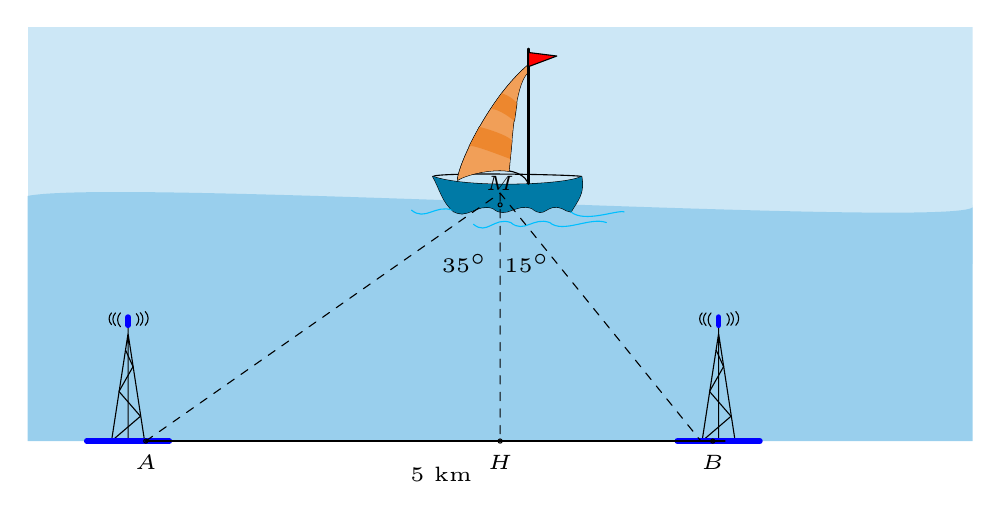
\begin{tikzpicture}[line join=round, line cap=round,scale=1.5,transform shape]
			\clip (-4,-1.5) rectangle (4,2.5);
			\fill[color=lightcornflowerblue!50] (-4,3)rectangle (4,.5);
			%\draw[fill=lightcornflowerblue!50] (-4,3)rectangle (4,.5);
			\def\N{ %nước biển
				(-4,1)
				..controls +(160:1) and +(-40:.4) ..(4,1)--(4,-1)--(-4,-1)--cycle
				;}
			%\draw \N;
			\fill[lightcornflowerblue] \N;
			
			\tikzset{thuyen_a/.pic={%Buồm
					\def\T{ 
						(.8,1.95)
						..controls +(-140:1.4) and +(85:.5) ..  (-1.2,-1.3)
						..controls +(40:.5) and +(100:.65) ..(.8,-1.45)--cycle
						;}
					\def\M{ 
						(.8,1.95)
						..controls +(-140:1.4) and +(85:.5) ..  (-1.2,-1.3)
						..controls +(30:.4) and +(170:.4) ..(.25,-1.05)
						..controls +(85:1.4) and +(-140:.45) ..  (.8,1.75)
						;}
					\def\B{ %buồm màu đậm
						(.05,1.15)
						..controls +(-20:.2) and +(100:.1) ..  (.47,0.85)
						..controls +(-130:.01) and +(80:.1) ..(.4,0.37)
						..controls +(130:.01) and +(10:.2) ..  (-.25,.7)--cycle
						%-----
						(-.58,.2)
						..controls +(-15:.5) and +(100:.1) ..  (.33,-.2)--(.28,-.7)
						..controls +(-130:.01) and +(80:.1) ..(-.87,-.35)--cycle
						;}
					\def\c{ %vòng cung thân thuyền
						(-1.9,-1.2)
						..controls +(40:.2) and +(150:.1) ..(2.3,-1.2);
					}
					\def\t{ %thân thuyền
						(-1.3,-2.2)
						..controls +(140:.45) and +(-60:.4) ..(-1.9,-1.2)
						..controls +(-20:1) and +(-150:.5) ..  (2.3,-1.2)
						..controls +(-80:.5) and +(60:.4) ..(2,-2.2)
						..controls +(160:.1) and +(-40:.1) ..(1.75,-2.1)
						..controls +(160:.5) and +(-40:.5) ..(.9,-2.1)
						..controls +(160:.5) and +(-40:.5) ..(-.2,-2.1)
						..controls +(160:.5) and +(-40:.5) ..(-1.35,-2.15)
						;}
					\def\S{ %sóng
						(-1.35,-2.15)
						..controls +(160:.5) and +(-40:.5) ..(-2.5,-2.15)
						(3.5,-2.2)
						..controls +(160:.2) and +(-40:.5) ..(2,-2.2)
						%----
						(3,-2.5)
						..controls +(160:.5) and +(-40:.5) ..(1.4,-2.5)
						..controls +(160:.5) and +(-40:.5) ..(.3,-2.5)
						..controls +(160:.5) and +(-40:.5) ..(-.75,-2.55)
						;}
					\draw \c;
					\draw \t;
					\draw \T;
					\draw \M;
					\draw \B;
					\draw[color=deepskyblue] \S;
					\fill[cadmiumorange!80] \M;
					\fill[cadmiumorange] \B;
					\fill[cerulean] \t;
					
					%Cờ, cột
					\draw[line width=1] (.8,2.4)--(.8,-1.4) ;
					\draw[fill=red] (.8,2.3)--(1.6,2.2)--(.8,1.9)--cycle;
			}}
			\tikzset{Angtenn/.pic={
					{
						\draw (0.5,0)--(0.5,1.5)(0.5,1.3)--(0.3,0)--(0.7,0)--cycle;
						\draw (0.3,0)--(0.65,0.3)--(0.39,0.6)--(0.56,0.9)--(0.47,1.1);
						\draw[line width=2pt,color=blue] (0,0)--(1,0) (0.5,1.4)--(0.5,1.5);
						\foreach \i in {1,1.08,1.18}{
							\draw (\i*0.6,1.4) arc (-45:45:\i*0.1);}
						\foreach \i in {1.18,1.08,1}{\draw(0.6*\i-0.3,1.55) arc (135:225:\i*0.1);}	 
				}}
				%	\draw \N;
				%\fill[black!70!] \N;
				\def\Q{ %quần
					(-3.045,-.9)
					..controls +(120:.01) and +(-30:0) .. (-3.04,-1.04)
					-- (-3.1,-1.038)
					..controls +(80:.07) and +(-10:0.01) .. (-3.13,-.94)--(-3.124,-.9)--cycle
					(-3.14,-1.04)--(-3.12,-1.04)
					..controls +(80:.07) and +(-10:0.01) .. (-3.134,-.96)--cycle
					;}
				
			}
			\path 
			(0,1.6)pic[scale=.3]{thuyen_a}
			(-3.5,-1)pic[scale=0.7]{Angtenn} 
			(1.5,-1)pic[scale=0.7]{Angtenn}
			;
			\draw[dashed] (-3,-1)--(0,1.1)--(1.7,-1) (0,1.1)--(0,-1) ;
			\draw[black,line width=1] (-3,-1)--(1.9,-1);
			\node at (-0.5,-1.1) [below]{ \tiny $5$ km};
			\node at (-0.3,0.3) [above]{\tiny $35^\circ$};
			\node at (0.23,0.3) [above]{\tiny $15^\circ$};
			\draw (-3,-1) node[below]{\tiny $A$} circle (0.5pt);
			\draw (0,1.) node[above]{\tiny $M$} circle (0.5pt);
			\draw (1.8,-1) node[below]{\tiny $B$} circle (0.5pt);
			\draw (0,-1) node[below]{\tiny $H$} circle (0.5pt);
		\end{tikzpicture}
	\end{center}
	\begin{listEX}
		\item  Tính khoảng cách $MH$ từ con tàu đến đường thẳng $AB$  nối hai ngọn hải đăng.
		\item Tính khoảng cách $MA$ từ con tàu đến ngọn hải đăng thứ nhất  và khoảng cách $MB$ từ con tàu đến ngọn hải đăng thứ hai.
		
	\end{listEX}
	\loigiai{ 
		\begin{listEX}
			\item  Khoảng cách từ con tàu đến đường thẳng nối hai ngọn hải đăng là $MH$ ($MH \perp AB$).\\
			Xét tam giác $AMH$ vuông tại $H$ có 
			\[\tan 35^\circ=\dfrac{AH}{MH}\Rightarrow AH= MH \cdot \tan 35^\circ.\]
			Xét tam giác $BMH$ vuông tại $H$ có 
			\[\tan 15^\circ=\dfrac{BH}{MH}\Rightarrow BH= MH \cdot \tan 15^\circ.\]
			Ta có 
			\begin{eqnarray*}
				AH+BH=AB&\Leftrightarrow &MH \cdot \tan 35^\circ+MH \cdot \tan 15^\circ=5\\
				&\Leftrightarrow& MH=\dfrac{5}{\tan 15^\circ+\tan 35^\circ}\approx 5{,}16 \ \text{(km)}.
			\end{eqnarray*}
			\item Khoảng cách từ con tàu đến ngọn hải đăng thứ nhất  là $MA$.\\
			Xét tam giác $MAH$ vuông tại $H$ có
			\[\cos 35^\circ=\dfrac{MH}{MA}\Rightarrow MA=\dfrac{MH}{\cos 35^\circ}=\dfrac{5}{\left(\tan 15^\circ+\tan 35^\circ\right)\cos 35^\circ}\approx 6{,}3 \ \text{(km).}\]
			Khoảng cách từ con tàu đến ngọn hải đăng thứ hai là $MB$.\\
			Xét tam giác $MBH$ vuông tại $H$ có 
			\[\cos 15^\circ=\dfrac{MH}{MB}\Rightarrow MB=\dfrac{MH}{\cos 15^\circ}=\dfrac{5}{\left(\tan 15^\circ+\tan 35^\circ\right)\cos 15^\circ}\approx 5{,}35 \ \text{(km).}\]
			
		\end{listEX}
		
	}
	
\end{ex}
\begin{ex}[Trích đề kiểm tra Toán khối 10 GHK1 NH24-25-THPT Nguyễn Thái Bình]%[0H4V3-2]%[Dự án đề cương 3 khối NH24-25 - Đợt 2 - Vũ Ngọc Hào]
	\immini{Trên nóc tòa nhà có một cột ăng-ten $BC$ cao $6$ m. Từ vị trí $A$ cao $8$ m so với mặt đất, một người quan sát có thể nhìn thấy đỉnh $B$ và chân $C$ của cột Ăng-ten, với hai góc tương ứng là $\widehat{DAB}=50^{\circ}$ và $\widehat{DAC}=40^{\circ}$ so với phương nằm ngang $AD$. Tính chiều cao $CH$ của toà nhà (làm tròn đến chữ số thập phân thứ nhất).
	}
	{\begin{tikzpicture}[scale=.4, font=\footnotesize, line join=round, >=stealth,thick] 
			\coordinate (O) at (0,0); \def\nhathap{1} %so tang nha thap 
			\def\nhacao{5} %so tang nha cao 
			\def\kc{10} %khoang cach 2 nha 
			\def\dai{1} %chieu dai 1 khoi 
			\def\cao{2} %chieu cao 1 khoi 
			\coordinate (H) at (\kc,0); 
			\newcommand{\xaynha}[2]{ \draw[very thick] (#1,#2)rectangle(#1+\dai,#2+\cao); \draw[very thick,fill=black] (#1,#2)rectangle(#1+\dai,#2+0.25*\cao); \draw[very thick] (#1+0.2*\dai,#2+0.25*\cao)rectangle(#1+0.8*\dai,#2+0.9*\cao); } % %Xay nha thap 
			\foreach \j in {1,...,\nhathap}{ \foreach \i in {0,...,4}{ \xaynha{\i*1.1}{\j*\cao} } } \draw[line width=0.2cm] (-0.1,\cao*\nhathap+\cao)--(5*\dai*1.1,\cao*\nhathap+\cao); \foreach \j in {1,...,\nhacao}{ \foreach \i in {0,...,4}{ \xaynha{\i*1.1+\kc}{\j*\cao} } } 
			\draw[line width=0.2cm] (-0.1+\kc,\cao*\nhacao+\cao)--(5*\dai*1.1+\kc,\cao*\nhacao+\cao); 
			\coordinate (A) at (5*\dai*1.1,\cao*\nhathap+\cao+0.1); \draw (A) node[above left]{$A$}; \coordinate (C) at (\kc,\cao*\nhacao+\cao); \draw (C) node[above right]{$C$}; 
			\coordinate (B) at ($(C)+(0,2)$); 
			\draw (B) node[above]{$B$}; 
			\coordinate (H) at (\kc,\cao); \draw (H) node[below]{$H$};
			\coordinate (D) at (\kc,\cao*\nhathap+\cao+0.1); \draw (D) node[above left]{$D$}; 
			\draw[very thick] (-0.5,\cao)--(\kc+5*\dai*1.2,\cao); 
			\draw [dashed](A)--(D); 
			\draw (B)--(A)--(C);
			\draw[line width=0.07cm] (C)--(B); 
			\draw ($(B)+(135:0.5cm)$)--($(B)+(-45:0.5cm)$); 
			\draw pic[draw,angle radius=7mm] {angle=D--A--B}; 
			\draw pic[draw,angle radius=3mm] {angle=D--A--C}; 
	\end{tikzpicture}}
	\loigiai{
		Từ hình vẽ, suy ra $\widehat{BAC}=10^\circ$ và \[\widehat{ABD}=180^\circ-\left(\widehat{BAD}+\widehat{ADB}\right)=180^\circ-\left(50^\circ+90^\circ\right)=40^\circ.\]
		Áp dụng định lí sin trong tam giác $ABC$ ta có
		\[\dfrac{BC}{\sin \widehat{BAC}}=\dfrac{AC}{\sin \widehat{ABC}} \Rightarrow AC= \dfrac{BC\cdot \sin \widehat{ABC}}{\sin \widehat{BAC}}=\dfrac{6\cdot \sin 40^{\circ}}{\sin 10^{\circ}} \approx 22{,}2 \text{ m}.\]
		Trong tam giác vuông $ADC$, ta có 
		\[\sin \widehat{CAD}=\dfrac{CD}{AC} \Rightarrow CD=AC\cdot \sin \widehat{CAD}=14{,}3 \text{ m}.\]
		Vậy $CH=CD+DH=14{,}3+8=22{,}3$ m.}
\end{ex}
\begin{ex}%[0D3V2-6]
	\immini{Ông Tiến có một mảnh đất hình tam giác vuông $ABC$ có diện tích $125$ m$^2$. Ông Tiến có ý định đào ao thả cá có dạng hình chữ nhật trên khu đất của mình (như hình vẽ). Hỏi rằng ông Tiến có thể đào một cái ao với diện tích lớn nhất là bao nhiêu?}
	{\begin{tikzpicture}[>=stealth,line join=round,line cap=round,font=\footnotesize,scale=1]
			\path (0,0) coordinate (A)
			(0,3) coordinate (B)
			(6,0) coordinate (C)
			(3.5,1.25) coordinate (E)
			; 
			\draw (A)--(B)--(C)--(A) (3.5,0)--(E)--(0,1.25)
			;
			\path (1.5,1) node[below]{$\text{Ao cá}$};
			\foreach \p/\r in {A/180,B/90,C/0,E/60}
			\fill (\p) circle (1pt) node[shift={(\r:3mm)}]{$\p$};
	\end{tikzpicture}	}
	\loigiai{
		\begin{center}
			\begin{tikzpicture}[>=stealth,line join=round,line cap=round,font=\footnotesize,scale=1]
				\path (0,0) coordinate (A)
				(0,3) coordinate (B)
				(6,0) coordinate (C)
				(3.5,1.25) coordinate (E)
				(3.5,0) coordinate (G)
				(0,1.25) coordinate (H)
				; 
				\draw (A)--(B)--(C)--(A) (G)--(E)--(H)
				;
				\path (1.5,1) node[below]{$\text{Ao cá}$};
				\foreach \p/\r in {A/180,B/90,C/0,E/60,H/180,G/-90}
				\fill (\p) circle (1pt) node[shift={(\r:3mm)}]{$\p$};
			\end{tikzpicture}
		\end{center}
		Giả sử ao cá hình chữ nhật $AHEG$ như hình vẽ. Diện tích ao là $S=AH\cdot HE$.\\
		Đặt $x=\dfrac{BE}{BC}$ $(0<x<1)$.\\
		Theo Talet ta có $\dfrac{AH}{AC}=\dfrac{BE}{BC}=x\Rightarrow AH=x\cdot AC$ 
		và \\ $\dfrac{HE}{AB}=\dfrac{CE}{BC}=\dfrac{BC-BE}{BC}=1-x\Rightarrow HE=(1-x)\cdot AB$.\\
		Khi đó $S=AH\cdot HE=x(1-x)AB\cdot AC=-250x^2+250x$.\\
		Ta xét hàm số $S=-250x^2+250x$ với $x\in (0;1)$.\\
		Ta có bảng biến thiên như sau
		\begin{center}
			\begin{tikzpicture}
				\tkzTabInit[nocadre=true,lgt=1.2,espcl=3.5,deltacl=0.6]
				{$x$ /1.1,$y$ /2.5}
				{$0$,$\frac{1}{2}$,$1$}
				\tkzTabVar{-/$0$,+/$62{,}5$,-/$0$}
			\end{tikzpicture}
		\end{center}
		Vậy ông Tiến có thể đào ao thả cá với diện tích lớn nhất là $62{,}5$ m$^2$ khi điểm $E$ là trung điểm của cạnh huyền $BC$.	
	}
\end{ex}
